\documentclass[12pt,a4paper,oneside]{book}
\usepackage[utf8]{inputenc}
\usepackage[T2A,T1]{fontenc}
\usepackage[english,russian]{babel}
\usepackage{geometry}
\geometry{left=24mm,right=19mm,top=21mm,bottom=23mm}
\usepackage{amsmath,amssymb,mathtools,bm}
\usepackage{booktabs,longtable,tabularx,array,multirow}
\usepackage{graphicx,float,caption,subcaption,pdfpages}
\usepackage{pdflscape}
\usepackage{xcolor,listings,fancyvrb}
\usepackage{enumitem,microtype,setspace}
\microtypesetup{expansion=false}
\usepackage{hyperref}
\usepackage[nameinlink,capitalise,noabbrev]{cleveref}
\usepackage{fancyhdr}
\usepackage{url}
\graphicspath{{manual_assets/}}
\setstretch{1.13}
\setlength{\parindent}{1.25cm}
\setlength{\parskip}{0.15em}
\setlist{nosep,leftmargin=1.6em}
\hypersetup{colorlinks=true,linkcolor=blue!45!black,citecolor=blue!45!black,urlcolor=blue!55!black}
\lstset{basicstyle=\ttfamily\small,breaklines=true,frame=single,backgroundcolor=gray!6,
  columns=fullflexible,keepspaces=true,showstringspaces=false}
\pagestyle{fancy}\fancyhf{}\fancyhead[L]{BEM-CUDA}\fancyhead[R]{Руководство пользователя}
\fancyfoot[C]{\thepage}\setlength{\headheight}{15pt}
\newcommand{\code}[1]{\texttt{\detokenize{#1}}}
\newcommand{\vect}[1]{\bm{#1}}
\newcommand{\dd}{\mathop{}\!\mathrm d}
\newcommand{\iu}{\mathrm i}
\newcommand{\E}{\vect E}
\newcommand{\Hf}{\vect H}
\newcommand{\J}{\vect J}
\newcommand{\M}{\vect M}
\newcommand{\normal}{\widehat{\vect n}}
\newcommand{\trans}{\mathsf T}
\newcommand{\herm}{\mathsf H}
\newcommand{\important}[1]{\begin{quote}\colorbox{yellow!18}{\parbox{0.91\textwidth}{#1}}\end{quote}}
\newcommand{\csvsection}[2]{\begin{landscape}\section{#1}\VerbatimInput[fontsize=\tiny,frame=single]{#2}\end{landscape}}

\title{\textbf{BEM-CUDA}\\[0.4em]
Полное руководство пользователя и разработчика\\[0.7em]
\large Метод граничных элементов для рассеяния электромагнитных волн
на диэлектрических частицах}
\author{К.~С.~Сальников\\ Институт оптики атмосферы им. В.~Е.~Зуева СО РАН}
\date{Версия документа: 10 июля 2026 г.}

\begin{document}
\frontmatter
\maketitle
\thispagestyle{empty}
\vfill
\noindent\textbf{Назначение документа.} Руководство описывает физическую постановку,
математический формализм PMCHWT, дискретизацию RWG, вычисление сингулярных интегралов,
FMM-ускорение, итерационные решатели, ориентационное усреднение, форматы данных и
практический выбор параметров BEM-CUDA. Документ ориентирован как на пользователя,
которому нужен воспроизводимый расчёт матрицы Мюллера, так и на разработчика,
изменяющего вычислительное ядро.

\medskip
\noindent\textbf{Статус рекомендаций.} Численные рекомендации основаны на текущей версии
кода и сохранённых экспериментальных таблицах. Экспериментальные режимы явно отмечены.
Наличие команды в программе не означает, что её следует применять в публикационном
расчёте. Основной критерий пригодности результата --- истинная невязка и независимая
сходимость наблюдаемых величин, а не только завершение процесса без ошибки.

\clearpage
\chapter*{Краткая памятка}
\addcontentsline{toc}{chapter}{Краткая памятка}
Для первого контролируемого расчёта сферы:
\begin{lstlisting}[language=bash]
./bin/bem_cuda_fmm --shape sphere --ka 5 --ri 1.6 0 \
  --ref 4 --single --ntheta 181 --solver fmm \
  --system balanced --quad 7 --fmm-digits 6 \
  --gmres-tol 1e-5 --gmres-restart 500 --max-leaf 128 \
  --out sphere_ka5.json
\end{lstlisting}
Для произвольной замкнутой поверхности:
\begin{lstlisting}[language=bash]
./bin/bem_cuda_fmm --obj particle.obj --ka 20 --ri 1.6 0.002 \
  --accurate --solver fmm --system balanced --single \
  --ntheta 181 --out particle_ka20.json
\end{lstlisting}
Перед длительным расчётом необходимо выполнить проверку сетки:
\begin{lstlisting}[language=bash]
./bin/bem_cuda_fmm --obj particle.obj --ka 20 --ri 1.6 0.002 \
  --mesh-quality-only --mesh-quality-report mesh_quality.json
\end{lstlisting}
Минимальный публикационный протокол включает: (1) сходимость по сетке; (2) сходимость
по квадратуре и точности FMM; (3) истинную невязку; (4) сходимость ориентационного
усреднения; (5) проверку энергетических и симметрийных ограничений; (6) независимый
эталон на сфере или ADDA для несферической частицы.

\tableofcontents
\listoffigures
\listoftables

\mainmatter
\part{Начало работы}

\chapter{Введение}
\section{Назначение BEM-CUDA}
BEM-CUDA решает частотную задачу рассеяния электромагнитной волны конечной
однородной диэлектрической частицей в однородной внешней среде. Геометрия задаётся
замкнутой ориентированной треугольной поверхностью. В отличие от объёмных методов,
неизвестные размещаются только на границе частицы. При характерном числе поверхностных
неизвестных $N$ решается комплексная система размера $2N$: первый набор коэффициентов
задаёт эквивалентный электрический ток, второй --- эквивалентный магнитный ток.

Главный выход программы --- угловая матрица Мюллера $M_{ij}(\theta)$ для одной
ориентации или после усреднения по ориентациям. Дополнительно сохраняются сведения о
сетке, выбранной интегральной системе, параметрах FMM/GMRES, истинной невязке,
занятой памяти и времени этапов. Эти метаданные являются частью результата: без них
невозможно доказать воспроизводимость и точность расчёта.

\section{Область применимости}
Текущая реализация предназначена для:
\begin{itemize}
\item однородных изотропных частиц с комплексным показателем преломления
  $m=n+\iu\kappa$;
\item сфер, гексагональных призм и произвольных OBJ-поверхностей;
\item плоской падающей волны;
\item дальнего поля и матрицы Мюллера;
\item одной ориентации, явной сетки углов Эйлера и ускоренного усреднения по $\alpha$;
\item плотного контрольного решения и FMM-ускоренного итерационного решения.
\end{itemize}
Код не следует без дополнительной верификации применять к незамкнутым поверхностям,
контактирующим телам, анизотропным и пространственно неоднородным материалам,
многослойным частицам, подложкам и ближнему полю. Сильно резонансные частицы и большие
$|m|$ требуют отдельного исследования сеточной и итерационной сходимости.

\section{Соглашения и единицы}
Используется временная зависимость $\exp(-\iu\omega t)$. Внешнее волновое число
$k=2\pi/\lambda$, размерный параметр
\begin{equation}
 ka_{\rm eq}=k a_{\rm eq},\qquad
 a_{\rm eq}=\left(\frac{3V}{4\pi}\right)^{1/3},
 \label{eq:size}
\end{equation}
где $V$ --- объём частицы. В CLI параметр называется \code{--ka}; в графиках
допустимо обозначение $ka_{\rm eq}$. OBJ автоматически нормируется к
$a_{\rm eq}=1$, поэтому абсолютные единицы длины не требуются. Все углы CLI задаются
в градусах, внутренние тригонометрические вычисления выполняются в радианах.

\chapter{Получение и сборка}
\section{Требования}
Рабочая конфигурация использует Linux, компилятор C++ с OpenMP, CUDA toolkit и GPU
архитектуры не ниже Volta. Проверенные ускорители --- Tesla V100 16~GB. Для анализа
JSON и построения графиков требуются Python, NumPy и Matplotlib. LaTeX нужен только
для сборки документации.

\section{Сборка FMM-версии}
Скрипт автоматически ищет совместимый CUDA toolkit:
\begin{lstlisting}[language=bash]
cd /path/to/BEM-CUDA
scripts/build_cuda_fmm.sh
./bin/bem_cuda_fmm --help
\end{lstlisting}
Явный toolkit задаётся переменной \code{CUDA_HOME}. Архитектура V100 соответствует
\code{sm\_70}. Сборка \code{fmm-only} исключает необязательные экспериментальные
backend-ы и является рекомендуемой для производственных прогонов.

\section{Проверка установки}
После сборки выполняются короткие тесты синтаксиса и CPU-эталона операторов:
\begin{lstlisting}[language=bash]
python3 tests/test_main_syntax_smoke.py
python3 tests/test_cpu_pmchwt_centroid_reference.py
\end{lstlisting}
Далее следует малый расчёт сферы и сравнение с теорией Ми. Нельзя начинать многосуточный
прогон произвольной частицы, пока этот контроль не проходит на той же машине и версии
бинарного файла.

\chapter{Запуск программы}
\section{Общая форма команды}
\begin{lstlisting}[language=bash]
./bin/bem_cuda_fmm --ka KA [geometry] [material] [orientations]
                    [accuracy] [solver] --out result.json
\end{lstlisting}
Единственный безусловно обязательный физический аргумент --- \code{--ka}. Однако
воспроизводимая команда всегда должна явно содержать материал, геометрию, систему,
квадратуру, точность FMM, допуск и размер перезапуска GMRES.

\section{Коды завершения и незавершённое решение}
Если истинная невязка не достигла допуска, программа записывает диагностический JSON,
но завершает работу с ошибкой. Такой файл нельзя автоматически включать в итоговое
усреднение. Переменная \code{BEM\_ALLOW\_NONCONVERGED=1} разрешает использовать его
только для диагностики. В научном расчёте эта переменная должна отсутствовать.

\section{GPU и параллельные задания}
Один процесс BEM обычно закрепляется за одной GPU через \code{CUDA\_VISIBLE\_DEVICES}.
Для ансамбля независимых размеров или ориентаций выгоднее запускать разные процессы на
разных картах, чем распределять один размер между четырьмя картами. Исключение ---
специальные пакетные сценарии ориентационного усреднения. Одновременный запуск двух
тяжёлых процессов на одной карте приводит к конкуренции за память и не считается
ускорением.

\part{Физическая и математическая постановка}

\chapter{Уравнения Максвелла и граничные условия}
\section{Гармонические поля}
В каждой однородной области $j\in\{e,i\}$ поля удовлетворяют
\begin{align}
 \nabla\times\E_j &= \iu\omega\mu_j\Hf_j, &
 \nabla\times\Hf_j &= -\iu\omega\varepsilon_j\E_j,\\
 \nabla\cdot(\varepsilon_j\E_j)&=0, &
 \nabla\cdot(\mu_j\Hf_j)&=0.
\end{align}
Здесь $e$ обозначает внешнюю среду, $i$ --- внутренность частицы,
$k_j=\omega\sqrt{\varepsilon_j\mu_j}$ и
$\eta_j=\sqrt{\mu_j/\varepsilon_j}$. Для немагнитной частицы во внешней среде с
единичным показателем $k_i=m k_e$ и $\eta_i=\eta_e/m$.

\section{Конкретные граничные условия}
Если на границе $\Gamma$ отсутствуют физические поверхностные заряды и токи, то
непрерывны касательные компоненты:
\begin{equation}
 \normal\times(\E_e-\E_i)=0,\qquad
 \normal\times(\Hf_e-\Hf_i)=0.
 \label{eq:bc}
\end{equation}
Нормаль направлена из частицы во внешнюю среду. Нормальные компоненты $\vect D$ и
$\vect B$ также непрерывны при отсутствии свободного поверхностного заряда и
магнитных монополей, но PMCHWT строится непосредственно из касательных следов.

\section{Падающая и рассеянная волны}
Во внешней области
$\E_e=\E^{\rm inc}+\E^{\rm sca}$ и
$\Hf_e=\Hf^{\rm inc}+\Hf^{\rm sca}$. Для плоской волны
\begin{equation}
 \E^{\rm inc}(\vect r)=\E_0 e^{\iu k_e\widehat{\vect k}\cdot\vect r},\qquad
 \Hf^{\rm inc}=\eta_e^{-1}\widehat{\vect k}\times\E^{\rm inc}.
\end{equation}
Рассеянное поле удовлетворяет условию излучения Зоммерфельда. Две независимые
линейные поляризации образуют два правых столбца одной и той же операторной системы.

\chapter{Принцип эквивалентности и поверхностные токи}
Эквивалентные токи не являются проводящими токами внутри диэлектрика. Это
математические поверхностные плотности, заменяющие действие объёма при сохранении полей
по выбранную сторону границы:
\begin{equation}
 \J=\normal\times\Hf,\qquad
 \M=-\normal\times\E.
 \label{eq:currents}
\end{equation}
Оба вектора касательны поверхности, поскольку их скалярное произведение с нормалью
равно нулю. Это не означает, что одна декартова компонента обязана исчезать: нулевой
является только нормальная проекция $\normal\cdot\J=\normal\cdot\M=0$.

Переход от полей к токам уменьшает размерность задачи: вместо трёхмерного поля во всём
объёме определяются две касательные векторные функции на двумерной границе. Цена этого
преимущества --- плотный не локальный оператор и сингулярные интегралы.

\begin{figure}[p]
\centering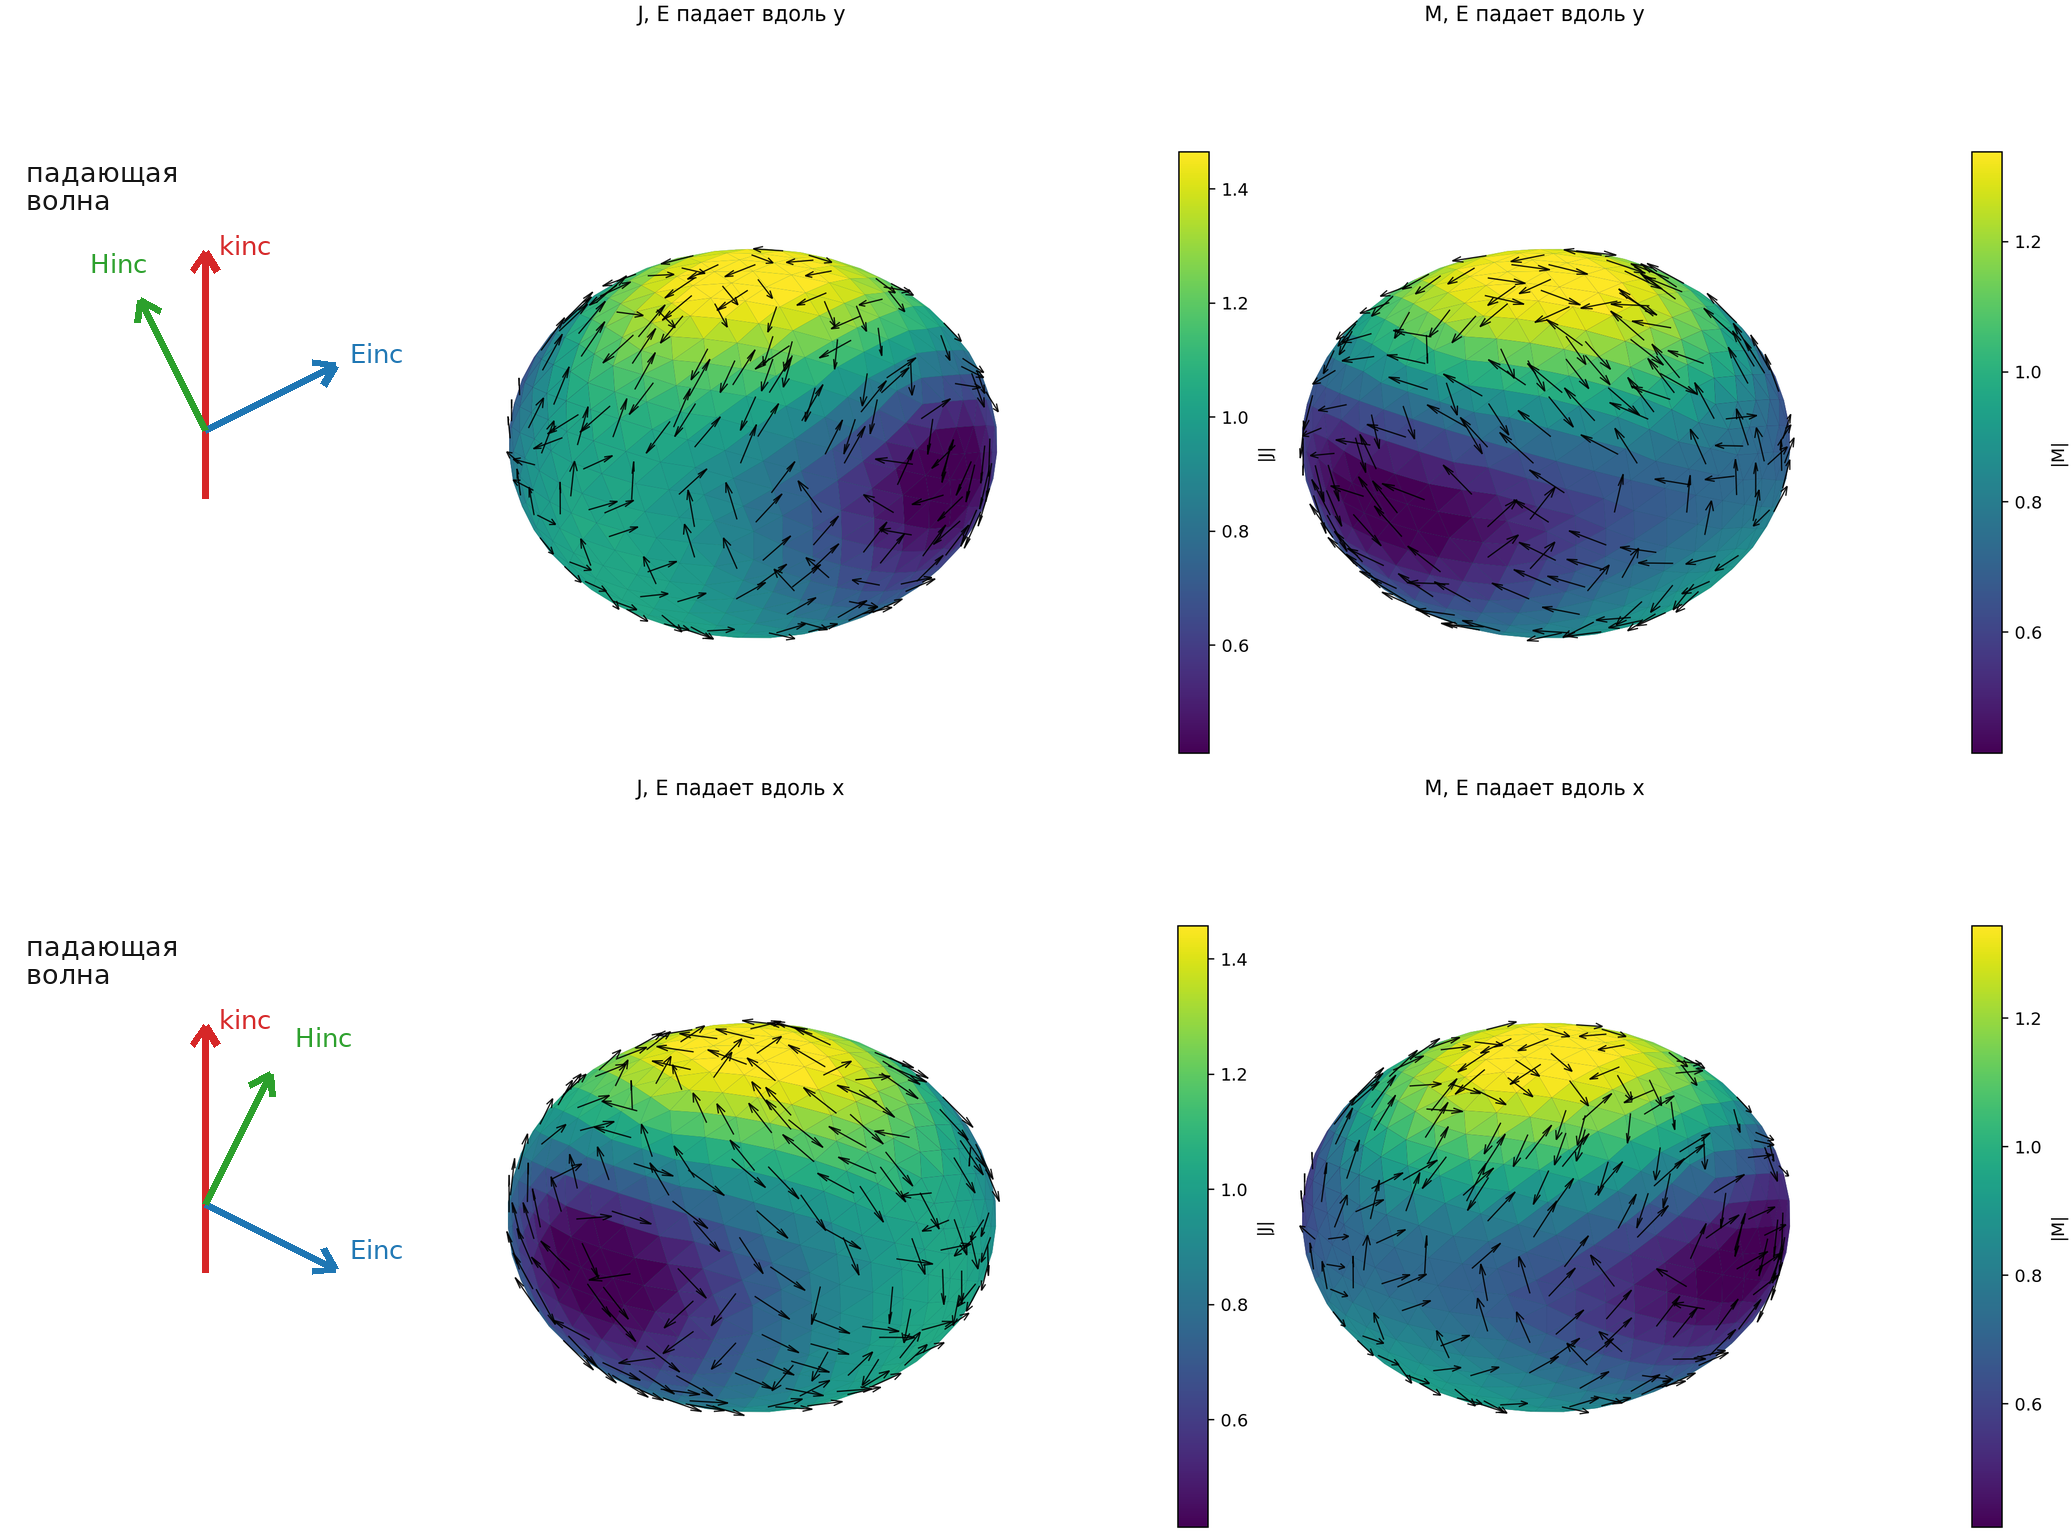
\includegraphics[width=0.96\textwidth]{fig_equiv_currents_sphere.png}
\caption{Эквивалентные поверхностные токи для двух поляризаций падающей волны.
Цвет показывает модуль тока, стрелки --- касательное направление. Цифры в обозначениях
$J_1,M_1$ относятся к первому возбуждению, а не к компоненте вектора.}
\label{fig:currents}
\end{figure}

\chapter{Интегральные операторы PMCHWT}
\section{Функция Грина}
Скалярная функция Грина уравнения Гельмгольца
\begin{equation}
 G_j(\vect r,\vect r')=\frac{e^{\iu k_j R}}{4\pi R},\qquad
 R=|\vect r-\vect r'|
\end{equation}
задаёт связь каждой точки поверхности со всеми остальными. Индекс $j$ определяет
волновое число внешней или внутренней среды.

\section{Операторы электрического и магнитного типа}
Для касательного тока $\vect X$ используем
\begin{align}
 \mathcal L_j[\vect X](\vect r)
 &=\iu k_j\int_\Gamma G_j\vect X\,\dd S'
 -\frac{1}{\iu k_j}\nabla\int_\Gamma G_j
   \nabla'_s\!\cdot\vect X\,\dd S',\label{eq:L}\\
 \mathcal K_j[\vect X](\vect r)
 &=\operatorname{p.v.}\int_\Gamma
   \nabla G_j(\vect r,\vect r')\times\vect X(\vect r')\,\dd S'.\label{eq:K}
\end{align}
Символ p.v. означает главное значение Коши. Поверхностная дивергенция
$\nabla_s\cdot\vect X$ действует вдоль поверхности. Первый член $\mathcal L$ связан с
векторным потенциалом, второй обеспечивает вклад скалярного потенциала и сохранение
заряда. Оператор $\mathcal K$ содержит градиент функции Грина и магнитный тип связи.

\section{Блочная система}
После суммирования внешних и внутренних граничных уравнений скачки взаимно уничтожаются.
В используемой знаковой конвенции система имеет вид
\begin{equation}
\begin{bmatrix}
 \eta_e L_e+\eta_i L_i & -(K_e+K_i)\\
 K_e+K_i & L_e/\eta_e+L_i/\eta_i
\end{bmatrix}
\begin{bmatrix}J\\M\end{bmatrix}
=
\begin{bmatrix}b_E\\b_H\end{bmatrix}.
\label{eq:pmchwt}
\end{equation}
Каждый символ $L_j,K_j$ в \cref{eq:pmchwt} означает уже дискретизированный оператор,
а не одно число. Вектор $b_E$ --- проекция касательного следа падающего электрического
поля, $b_H$ --- магнитного поля с согласованным знаком.

\section{Сбалансированная система}
Различие размерностей и масштабов электрического и магнитного токов ухудшает
обусловленность. Режим \code{balanced} использует масштаб магнитного неизвестного и
строки. Для комплексно-симметричных решателей дополнительно вводится точная замена
\begin{equation}
 \widetilde M=\iu |m|M,\qquad M=-\frac{\iu}{|m|}\widetilde M,
\end{equation}
и магнитная строка умножается на $\iu$. Тогда блоки $-K$ и $K$ переходят в одинаковые
перекрёстные блоки. На реальной сетке пылевой частицы дефект
$|x^TAy-y^TAx|/(\|x\|\|Ay\|+\|y\|\|Ax\|)$ уменьшился с порядка $10^{-3}$ до
$1.1\cdot10^{-9}$. Преобразование не меняет физическое решение при согласованном
преобразовании правой части и обратном восстановлении $M$.

\chapter{RWG-дискретизация}
\section{Базисные функции}
Каждому внутреннему ребру, общему для треугольников $T_n^+$ и $T_n^-$, соответствует
функция Рао--Уилтона--Глиссона
\begin{equation}
 \vect f_n(\vect r)=
 \begin{cases}
 \dfrac{l_n}{2A_n^+}(\vect r-\vect r_n^+),&\vect r\in T_n^+,\\[0.4em]
 \dfrac{l_n}{2A_n^-}(\vect r_n^--\vect r),&\vect r\in T_n^-,\\
 0,&\text{иначе}.
 \end{cases}
\end{equation}
Здесь $l_n$ --- длина общего ребра, $A_n^\pm$ --- площади треугольников,
$\vect r_n^\pm$ --- свободные вершины. Нормальная к ребру компонента внутри поверхности
непрерывна, поэтому RWG естественно представляет ток и его поверхностную дивергенцию.

Токи разлагаются как
\begin{equation}
 \J_h=\sum_{n=1}^N j_n\vect f_n,\qquad
 \M_h=\sum_{n=1}^N m_n\vect f_n.
\end{equation}
В схеме Галёркина теми же функциями тестируются интегральные уравнения. Для замкнутой
треугольной поверхности без дефектов число RWG равно числу рёбер.

\section{Почему качество треугольников важно}
Вытянутые треугольники создают сильно различающиеся нормы RWG, увеличивают ошибки
квадратуры и ухудшают обусловленность. Проверяются минимальный угол, отношение сторон,
отношение площадей соседей, двугранные углы, граничные и неманифолдные рёбра,
ориентация объёма и подозрительные близкие несмежные панели. Рекомендуемый строгий
порог: минимальный угол не ниже $20^\circ$ и аспект не выше 12. Нарушение порога не
доказывает ошибочность результата, но требует усиленного исследования сходимости.

\begin{figure}[p]
\centering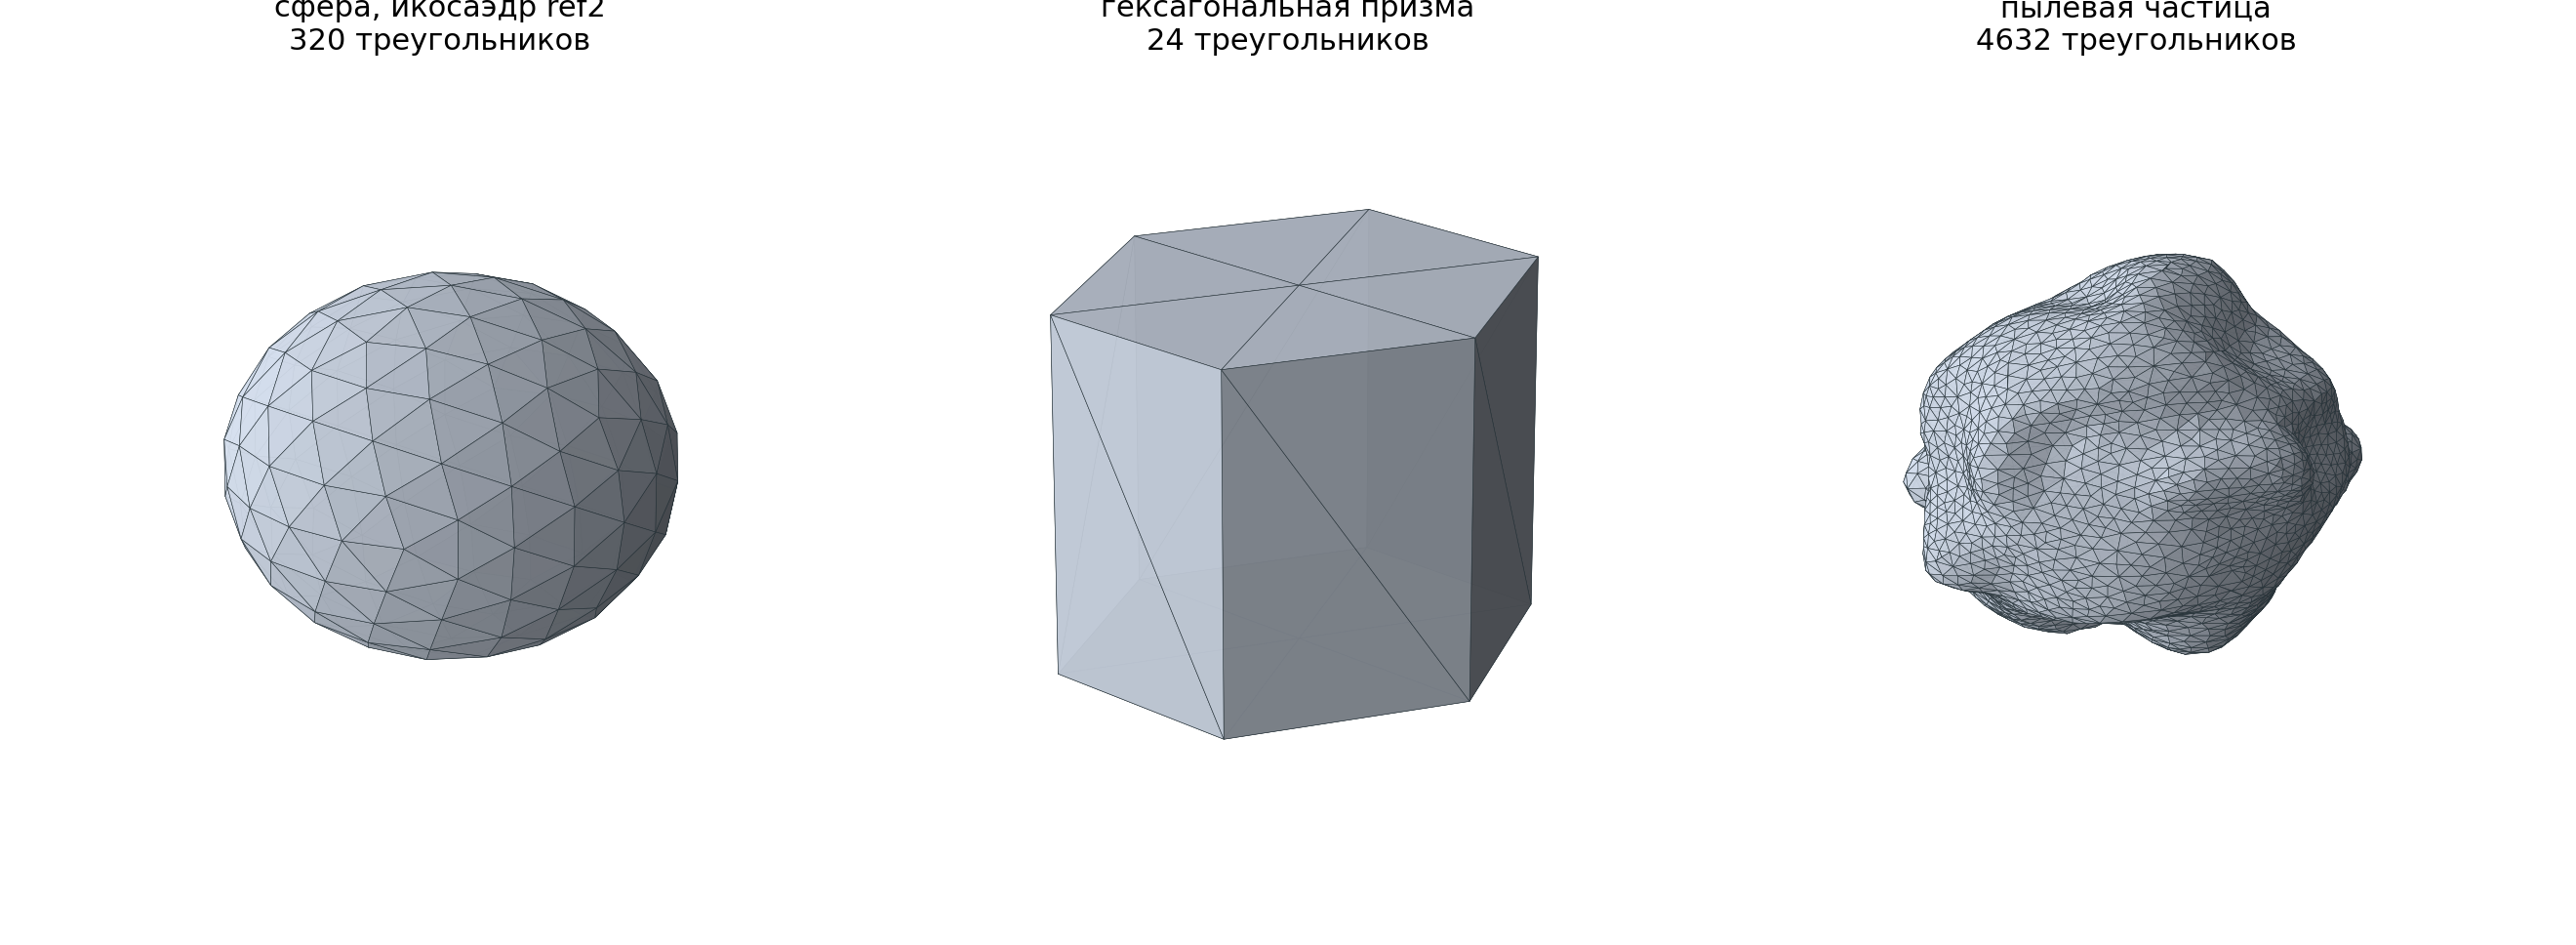
\includegraphics[width=0.95\textwidth]{fig_mesh_gallery.png}
\caption{Примеры треугольных сеток сферы, гексагональной призмы и пылевой частицы.
Сетка должна сохранять геометрию, быть замкнутой и согласованно ориентированной.}
\label{fig:meshes}
\end{figure}

\chapter{Сингулярные и близкие интегралы}
Пары панелей делятся на самодействующие, имеющие общее ребро, общую вершину,
геометрически близкие несмежные и дальние. Обычная гауссова квадратура достаточна лишь
для гладкой подынтегральной функции. Для сингулярных классов используются специальные
коррекции и локальное подразделение. Параметр \code{--quad} принимает 4, 7 или 13;
увеличение порядка не исправляет плохую геометрию автоматически.

Контроль квадратуры проводится сравнением наблюдаемых величин при $q=7$ и $q=13$ на
неизменной сетке и более точном FMM. Если изменение $M_{ij}$ превышает целевую ошибку,
нужно сначала локализовать углы и классы панелей, а не механически ужесточать GMRES.

\part{Вычислительные методы}

\chapter{Плотный метод и эталонный контроль}
Плотная сборка хранит все четыре блока и решает систему прямым LU. Память растёт как
$O(N^2)$, время факторизации --- как $O(N^3)$, поэтому режим применим только к малым
сеткам. Его роль --- независимый контроль знаков, масштабов, правой части и дальнего
поля. Совпадение плотного и FMM-решения при одной сетке отделяет ошибку ускорения от
ошибки геометрической дискретизации.

\chapter{Метод быстрых мультиполей}
\section{Иерархия}
Квадратурные источники группируются в октодерево. Взаимодействия близких ячеек
вычисляются непосредственно, дальние проходят этапы P2M, M2M, M2L, L2L и L2P.
Плосковолновое представление функции Грина сокращает стоимость одного матвека по
сравнению с плотным $O(N^2)$. Реальная асимптотика и константа зависят от $ka$,
глубины дерева, порядка разложения и распределения точек.

\section{Параметры точности}
\code{--fmm-digits d} задаёт требуемый порядок аппроксимации, а \code{--max-leaf}
управляет заполнением листа. Параметр digits не является гарантированным числом верных
цифр итоговой матрицы Мюллера: это внутренний параметр дальнего взаимодействия.
Рекомендуется $d=6$ для обычного контролируемого расчёта и $d=7$--8 для строгого
контроля OBJ. Выбор $d=3$ допустим только для предварительной диагностики.

\section{Симметрия FMM-оператора}
Аудит показал, что диагональные $L$-блоки сохраняют комплексную симметрию примерно до
$10^{-9}$. Исходный дефект полной PMCHWT-системы порядка $10^{-3}$ был связан не с FMM,
а с противоположными знаками перекрёстных блоков. После фазового преобразования полный
дефект также составляет около $10^{-9}$. Это открывает возможность коротких
комплексно-симметричных решателей, но не гарантирует их быструю сходимость.

\chapter{GMRES}
Для системы $Ax=b$ GMRES строит пространство Крылова
\begin{equation}
 \mathcal K_m(A,r_0)=\operatorname{span}\{r_0,Ar_0,\ldots,A^{m-1}r_0\}
\end{equation}
и минимизирует евклидову норму невязки. Арнольди требует ортогонализации нового вектора
по всему базису, поэтому стоимость и память растут с \code{--gmres-restart}. После
$m$ шагов выполняется перезапуск. Слишком малый $m$ вызывает стагнацию, слишком большой
увеличивает память и стоимость ортогонализации.

Основной рекомендуемый путь --- GPU-GMRES с истинной проверкой невязки. Допуск
\code{--gmres-tol} относится к $\|b-Ax\|_2/\|b\|_2$. Для матрицы Мюллера ошибка может
быть больше, особенно у слабых элементов, поэтому допуск решателя не равен ошибке
физической величины.

\chapter{Короткорекуррентные решатели}
\section{Общие преимущества и риск}
BiCGSTAB, CGS, TFQMR, QMR2, COCR и COCG хранят фиксированное число векторов и не
ортогонализуют длинный базис. Это уменьшает память, однако делает сходимость менее
монотонной и чувствительной к breakdown. Каждый режим обязан периодически вычислять
истинную невязку, сохранять лучшее решение и иметь безопасный откат на GMRES.

\section{QMR2}
QMR-CS-2 использует билинейные произведения без комплексного сопряжения,
$v^Tv$ и $p^TAp$, поэтому требует $A^T=A$, а не $A^HA=A$. После фазовой балансировки
условие выполнено с дефектом порядка $10^{-9}$. На сфере $ka=2$ QMR2 дал 67 матвеков
и 0.76~с против 53 и 0.59~с GPU-GMRES. На пылевой частице $ka=10$ при одинаковом
лимите QMR2 достиг $1.71\cdot10^{-3}$ за 316~с, а GMRES ---
$2.22\cdot10^{-4}$ за 290~с. Поэтому QMR2 остаётся экспериментальным.

\section{COCR}
COCR предназначен для комплексно-симметричной матрицы и использует один матвек на
итерацию. На малой сфере он дал 71 матвек и 0.80~с; симметричный локальный
предобуславливатель уменьшил это до 62 матвеков и 0.70~с, но GPU-GMRES остался быстрее.

\section{Блочный COCG}
Для двух поляризаций реализован истинный блок с матричными коэффициентами $2\times2$.
Он способен обмениваться направлениями между правыми частями, но при близкой линейной
зависимости поляризаций теряет ранг. На сфере тест остановился после 64 матвеков с
невязкой $1.30\cdot10^{-4}$. Для устойчивого развития необходим rank-revealing QR или
SVD на каждом шаге. Режим \code{block-cocg} не является производственной рекомендацией.

\chapter{Предобусловливание}
Текущий общий предобуславливатель использует локальные блоки ближних взаимодействий.
Односторонняя схема $P^{-1}A$ полезна GMRES, но разрушает комплексную симметрию и потому
не должна напрямую применяться в QMR2/COCR.

Для COCR реализована конгруэнтная схема
\begin{equation}
 \widetilde A=S^TAS,\qquad \widetilde b=S^Tb,\qquad x=S\widetilde x,
\end{equation}
где для каждого RWG берётся $S_i=D_i^{-1/2}$ от симметричного диагонального блока
$D_i\in\mathbb C^{2\times2}$. Численная проверка $S_i^TD_iS_i-I$ дала
$4.68\cdot10^{-15}$ на сфере и $8.44\cdot10^{-15}$ на пыли. Несмотря на формальную
корректность, на пыли этот локальный вариант ухудшил сходимость; он выключен по
умолчанию.

\part{Геометрия, ориентации и наблюдаемые величины}

\chapter{Задание геометрии}
\section{Сфера}
\code{--shape sphere --ref r} строит икосаэдрическую сферу. Каждый уровень делит грань
на четыре, поэтому число треугольников растёт примерно как $4^r$. Сфера служит главным
эталоном благодаря точному решению Ми. Нельзя выбирать ref только по доступной памяти:
для каждого $ka$ проводится сравнение минимум двух соседних уровней.

\section{Гексагональная призма}
\code{--shape hex\_prism --prism-aspect h} использует соглашение ADDA для отношения
высоты к поперечному размеру. Рёбра создают локальные особенности токов, поэтому
равномерная сетка может сходиться медленнее гладкой сферы. Экспериментальный
\code{--edge-refine} меняет сетку и требует отдельного контроля геометрии.

\section{OBJ}
OBJ должен быть триангулированным, замкнутым, двухмногообразным и ориентированным наружу.
Программа нормирует объём к единичной эквивалентной сфере. Плоское подразделение
\code{--subdiv} не восстанавливает кривизну исходной поверхности и потому может лишь
размельчить уже имеющуюся геометрическую ошибку.

\chapter{Ориентации частицы}
Ориентация задаётся углами Эйлера $\alpha,\beta,\gamma$. Для равномерного распределения
по $SO(3)$ интегральная мера пропорциональна
\begin{equation}
 \dd R=\frac{1}{8\pi^2}\dd\alpha\,\sin\beta\,\dd\beta\,\dd\gamma.
\end{equation}
Поэтому равномерная сетка по $\beta$ без веса $\sin\beta$ неверна. В явном файле
ориентаций каждая строка содержит $\alpha\ \beta\ \gamma\ [w]$ в градусах.

\code{--orient NA NB NG} решает $N_\alpha N_\beta N_\gamma$ правых частей.
\code{--alpha-avg N} использует то, что изменение $\alpha$ можно перенести в дешёвую
стадию дальнего поля: дорогие токи решаются по сетке $\beta,\gamma$, а $\alpha$
усредняется аналитически/дискретно в постобработке. Это ускорение корректно только при
согласованной поляризационной базе и проверено сравнением с явной сеткой.

\begin{figure}[p]
\centering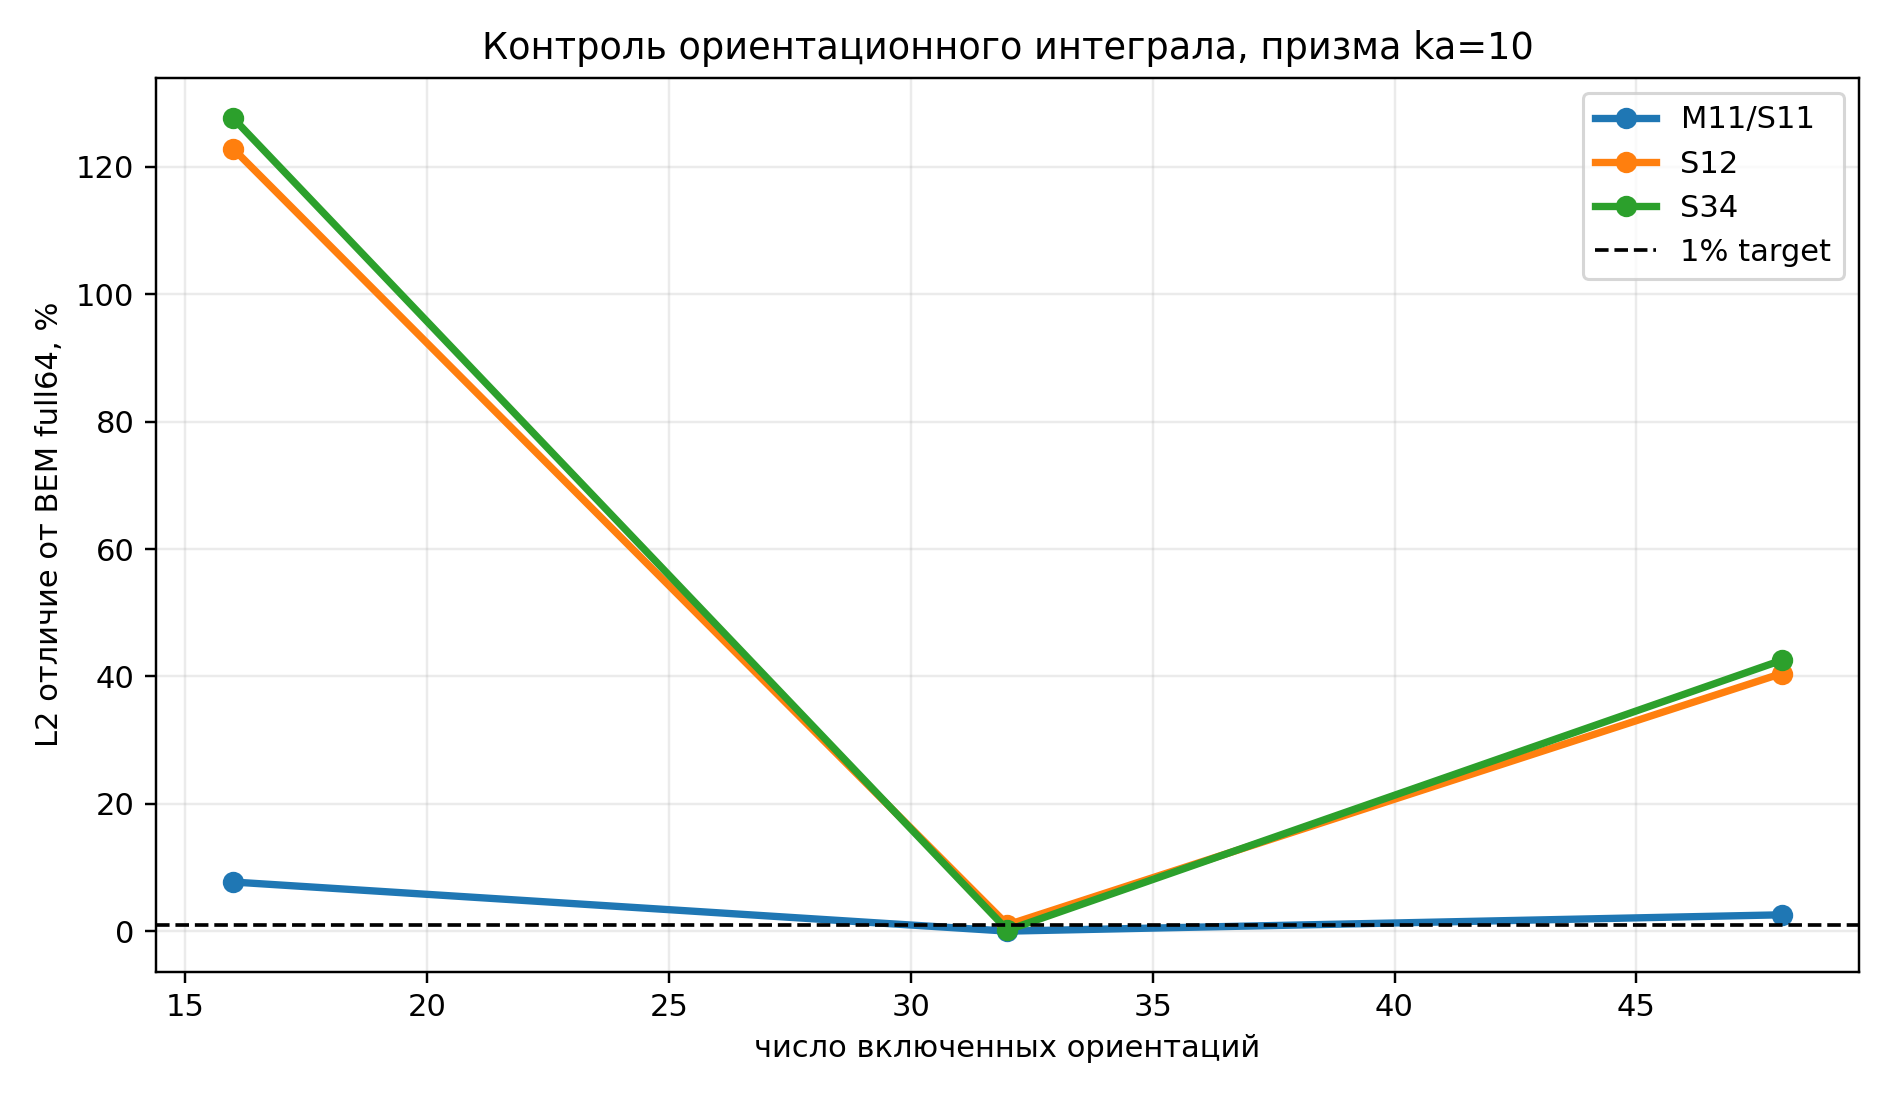
\includegraphics[width=0.94\textwidth]{fig_orientation_convergence.png}
\caption{Пример сходимости ориентационного усреднения. Оценивать следует не только
$M_{11}$, но и нормированные сильные и слабые элементы матрицы Мюллера.}
\label{fig:orientconv}
\end{figure}

\chapter{Амплитудная и Мюллерова матрицы}
В дальней зоне комплексные амплитуды двух поляризаций образуют матрицу рассеяния.
Матрица Мюллера переводит действительный вектор Стокса:
\begin{equation}
 \vect S_{\rm sca}=\frac{1}{k^2r^2}\,\mathbf M(\theta,\phi)\vect S_{\rm inc}.
\end{equation}
$M_{11}$ является фазовой функцией с точностью до принятой нормировки и не может быть
отрицательным. Отрицательный $M_{11}$ означает ошибку формул, индексов, усреднения или
данных. Остальные элементы могут менять знак. Для графиков $M_{11}$ применяют
логарифмическую шкалу, а остальные элементы удобно показывать как $M_{ij}/M_{11}$ на
линейной шкале.

Сравнение слабых элементов нельзя выполнять обычной поточечной относительной ошибкой
вблизи нулей. Используются взвешенная $L_2$-ошибка, абсолютная ошибка после нормировки
на интеграл $M_{11}$ и отдельный контроль сильных/слабых компонент.

\part{Точность, производительность и практические профили}

\chapter{Иерархия ошибок}
Полная ошибка включает геометрию, RWG-дискретизацию, квадратуру, FMM, итерационный
решатель, угловую сетку наблюдения и ориентационное усреднение. Уменьшение
\code{gmres-tol} не исправляет грубую поверхность. Увеличение \code{fmm-digits} не
исправляет недостаточный ref. Увеличение числа ориентаций не исправляет ошибку одной
ориентации.

Рекомендуемый порядок исследования:
\begin{enumerate}
\item проверить топологию и качество поверхности;
\item на малой сетке сравнить dense и FMM;
\item выбрать квадратуру и digits;
\item добиться истинной невязки;
\item уточнить поверхность при фиксированных параметрах оператора;
\item только затем исследовать ориентационное усреднение.
\end{enumerate}

\chapter{Метрики сравнения}
Для вектора значений $f_i$ и эталона $g_i$ вводится
\begin{equation}
 \varepsilon_{L_2}=\frac{\left[\sum_i w_i|f_i-g_i|^2\right]^{1/2}}
 {\left[\sum_i w_i|g_i|^2\right]^{1/2}}.
\end{equation}
Для фазовой функции веса включают сферическую меру $\sin\theta$. Интегральный контроль
\begin{equation}
 I_{11}=2\pi\int_0^\pi M_{11}(\theta)\sin\theta\,\dd\theta
\end{equation}
обнаруживает систематическую потерю бокового или обратного рассеяния. Совпадение только
вперёд недостаточно: узкий передний пик может доминировать в невзвешенной метрике.

\chapter{Проверка на сферах}
\begin{figure}[p]
\centering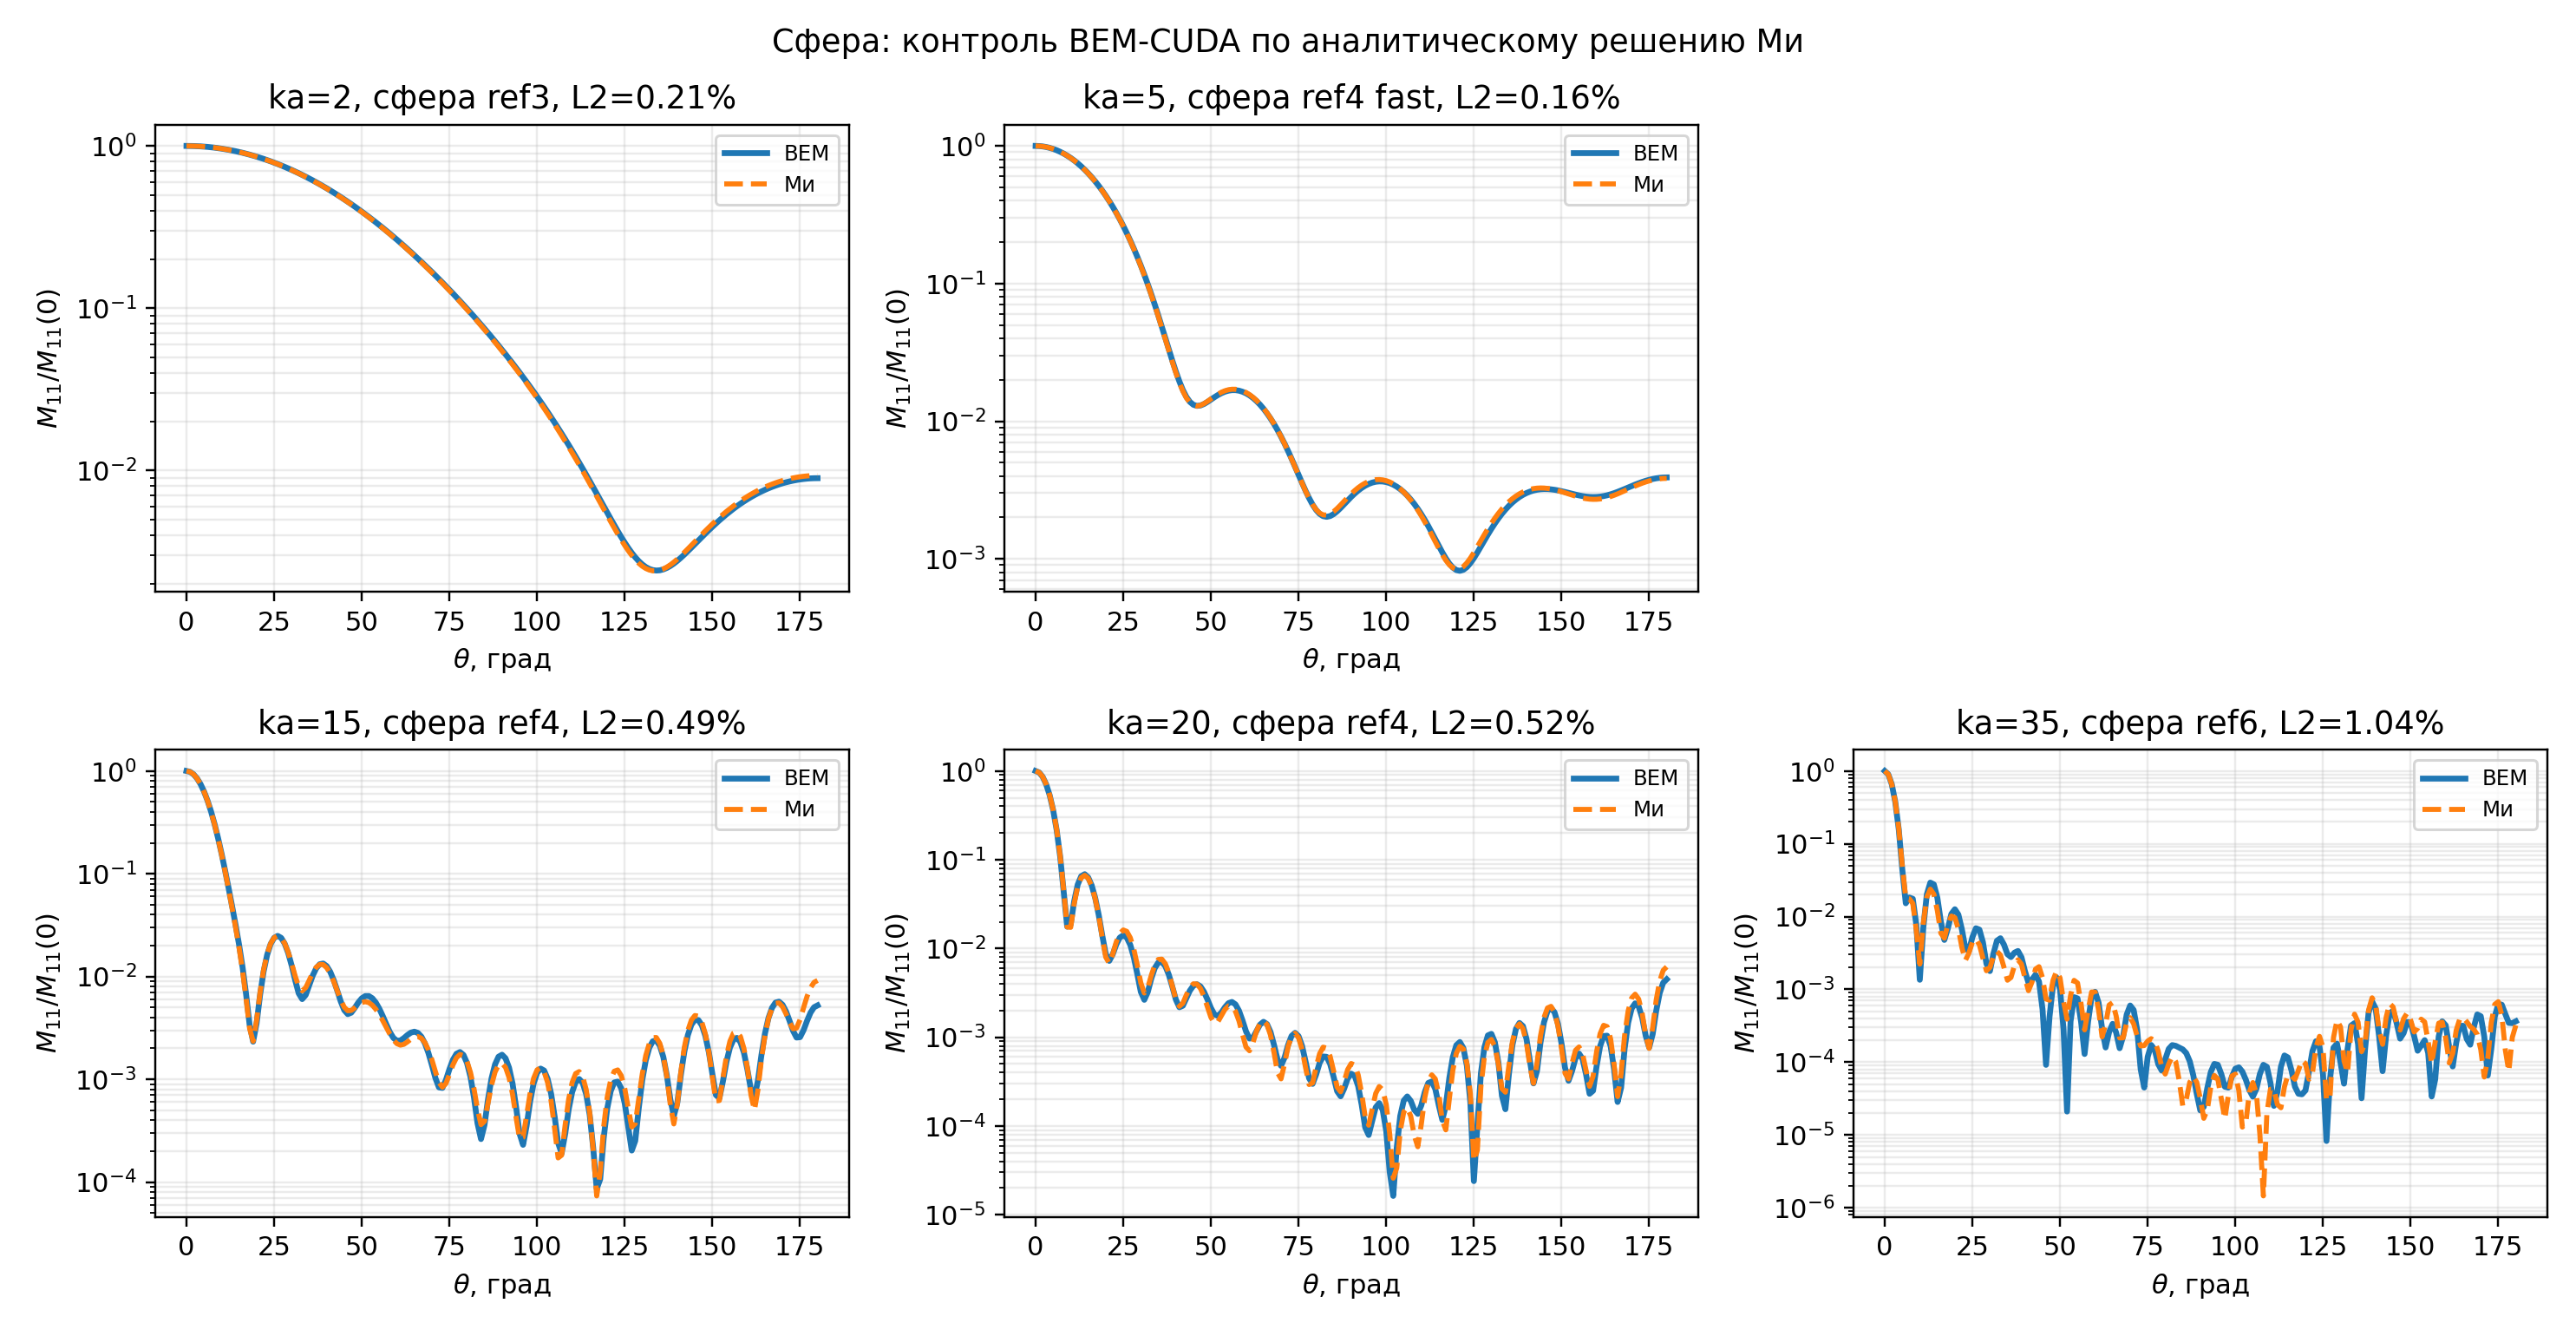
\includegraphics[width=0.98\textwidth]{fig_mie_validation_combined.png}
\caption{Сравнение BEM с теорией Ми на сферах. График следует читать вместе с таблицей
параметров сетки и невязки; одна визуальная близость кривых не является доказательством.}
\label{fig:mie}
\end{figure}
Сфера проверяет одновременно знаки PMCHWT, нормировку геометрии, поляризационную базу,
дальнее поле и матрицу Мюллера. Для больших $ka$ сферическая сетка должна уточняться,
пока изменение результата не станет меньше целевой ошибки. Точка, не прошедшая контроль,
не должна изображаться как обычная линия производительности.

\chapter{Сравнение с ADDA}
ADDA и BEM дискретизируют разные интегральные уравнения: ADDA --- объём, BEM --- границу.
Одинаковый объект означает совпадение физической поверхности, материала, $ka$, направления
волны, ориентаций, поляризационной базы и углов наблюдения, а не одинаковое число
неизвестных. Для честного сравнения необходимо использовать одну и ту же явную сетку
ориентаций или доказать эквивалентность ускоренного усреднения.

\begin{figure}[p]
\centering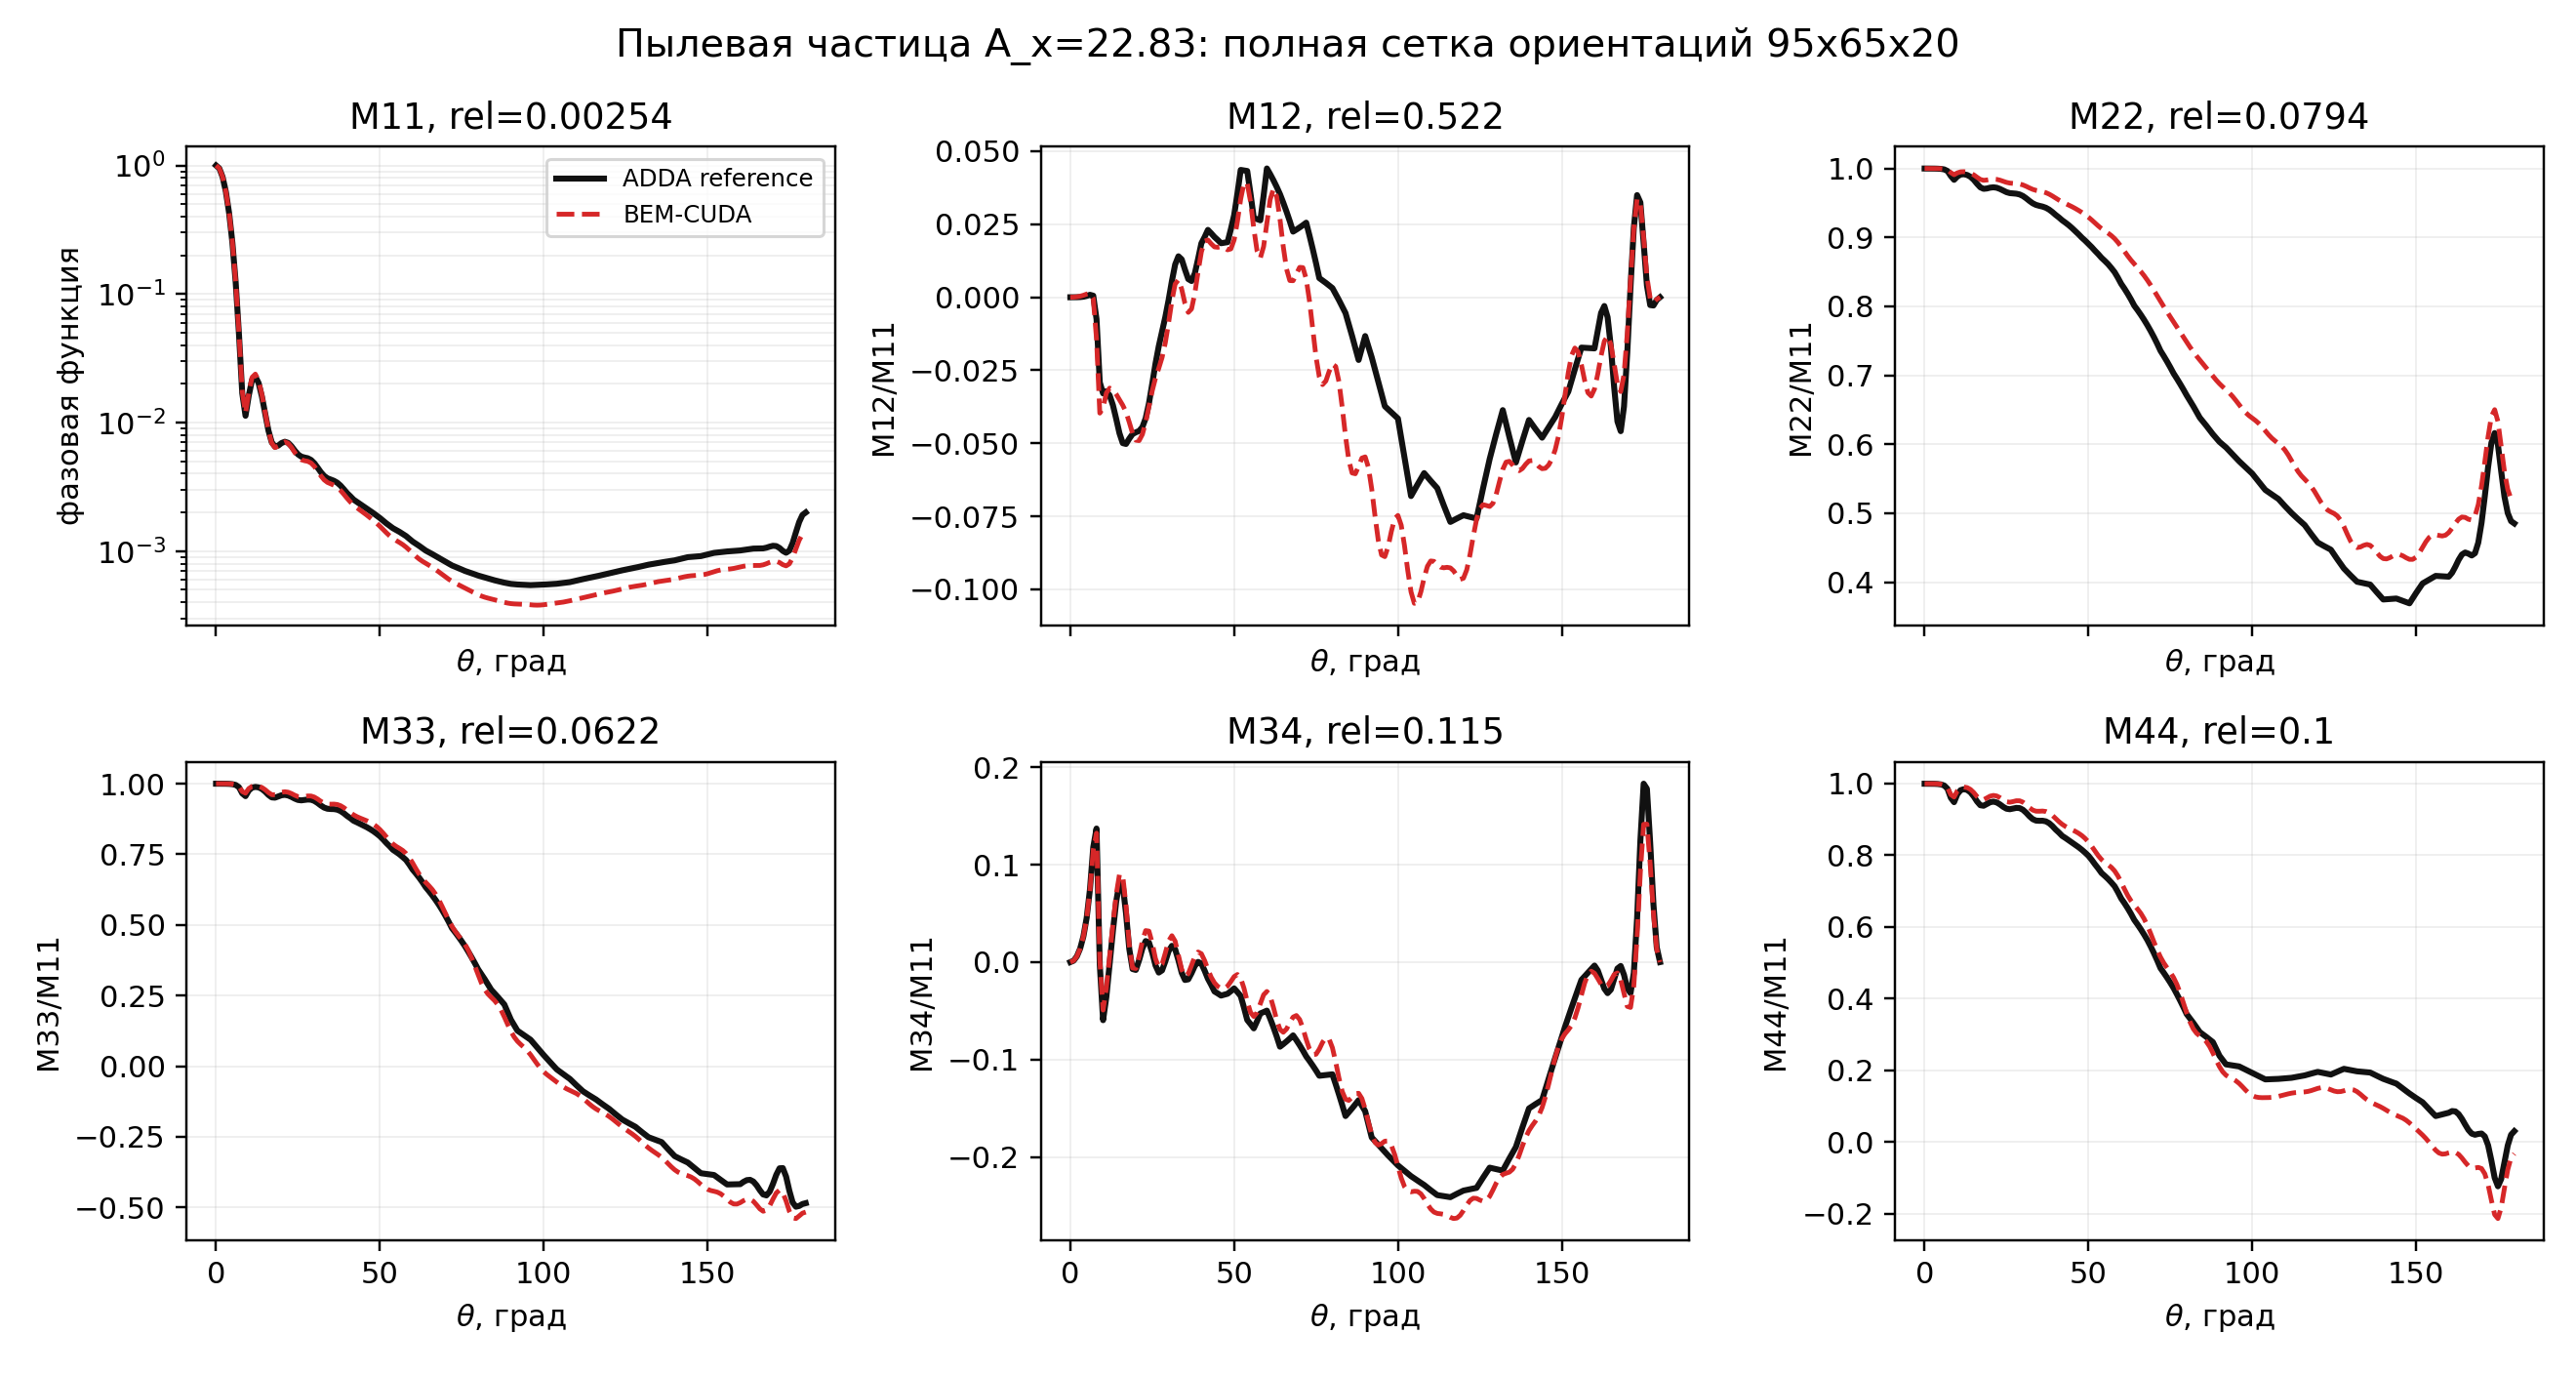
\includegraphics[width=0.98\textwidth]{fig_dust_fullgrid_compare.png}
\caption{Пример полного сравнения BEM и ADDA для пылевой частицы. Фазовая функция
показана логарифмически, остальные элементы нормированы на $M_{11}$.}
\label{fig:dustadda}
\end{figure}

\chapter{Память GPU}
Память FMM расходуется на квадратурные источники, дерево, переводы M2L, ближние пары,
рабочие буферы матвека и векторы решателя. GMRES дополнительно хранит базис порядка
\begin{equation}
 B_{\rm Krylov}\approx 2\,m\,(2N)\,16\ \text{байт}
\end{equation}
для двух поляризаций без учёта служебных массивов. Короткорекуррентные решатели уменьшают
эту часть, но не память дерева FMM.

\begin{figure}[p]
\centering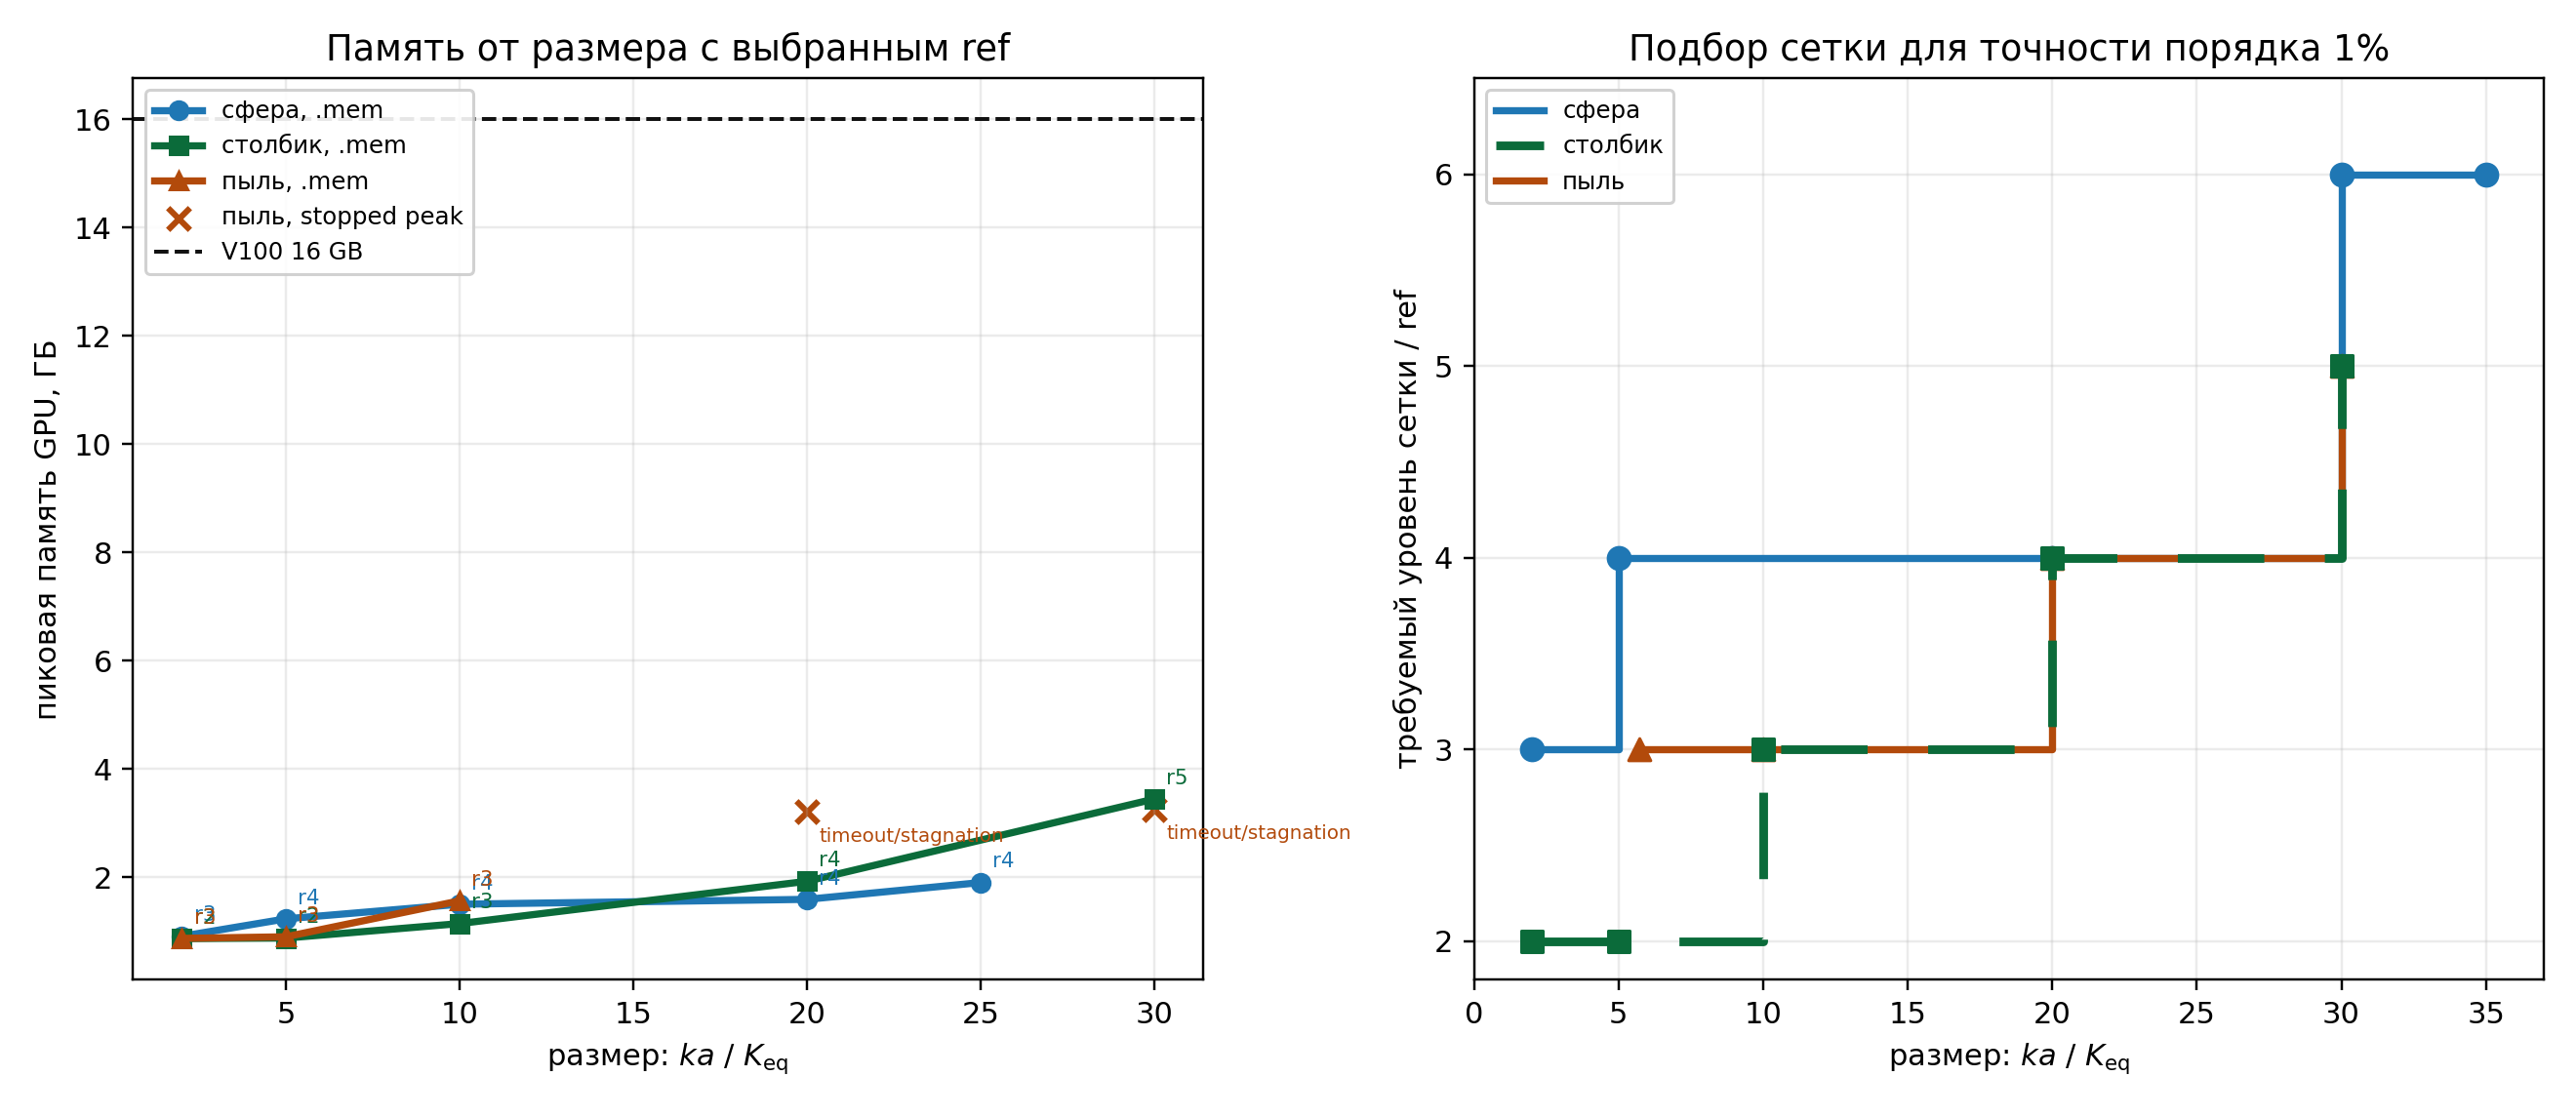
\includegraphics[width=0.96\textwidth]{fig_vram_forecast.png}
\caption{Экспериментальная зависимость видеопамяти от размера и дискретизации. Линии
следует интерпретировать только в пределах измеренного диапазона; форма и качество
сетки изменяют число RWG при одинаковом $ka$.}
\label{fig:vram}
\end{figure}

Перед запуском следует оставлять запас не менее 10--15\% VRAM. CUDA OOM обычно завершает
процесс, но перегрузка нескольких блоков питания или PCIe-моста может выключить весь
узел; это аппаратная проблема и не должна маскироваться уменьшением допуска решателя.

\chapter{Время расчёта}
Полное время состоит из построения сетки, инициализации FMM, коррекций, решения всех
правых частей и дальнего поля. Для одной геометрии и материала FMM-инициализацию следует
переиспользовать между ориентациями. Сравнение скоростей нормируется на одну GPU Tesla
V100 и одинаковый критерий точности.

\begin{figure}[p]
\centering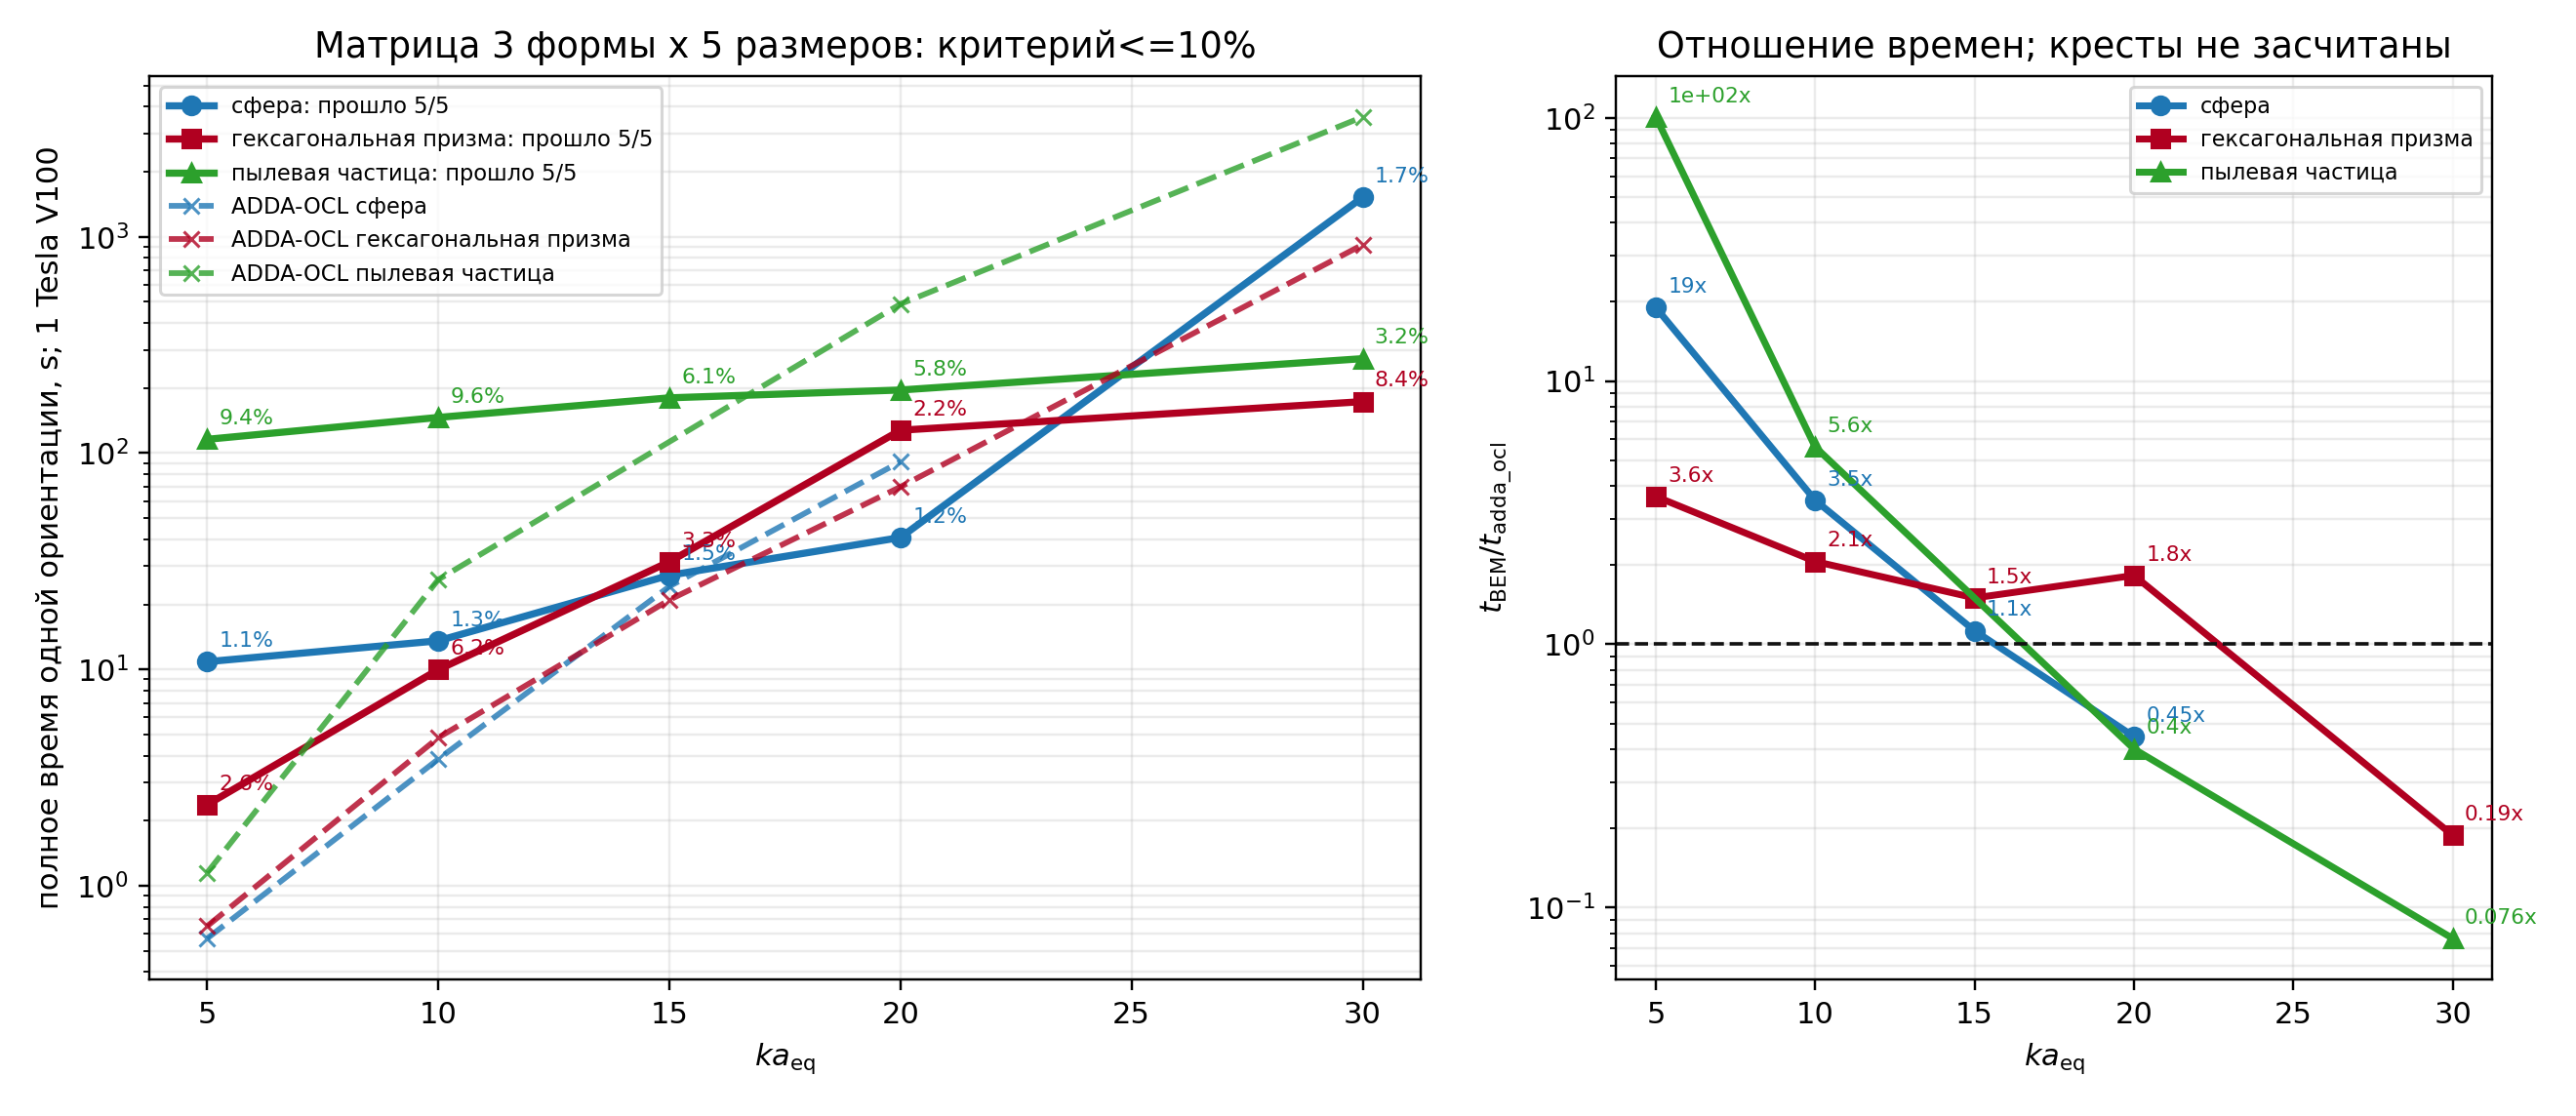
\includegraphics[width=0.96\textwidth]{fig_shape_single_time.png}
\caption{Измеренное время одной ориентации для разных форм. Рост определяется не только
$ka$, но и необходимым числом треугольников и числом итераций.}
\label{fig:time}
\end{figure}

\begin{figure}[p]
\centering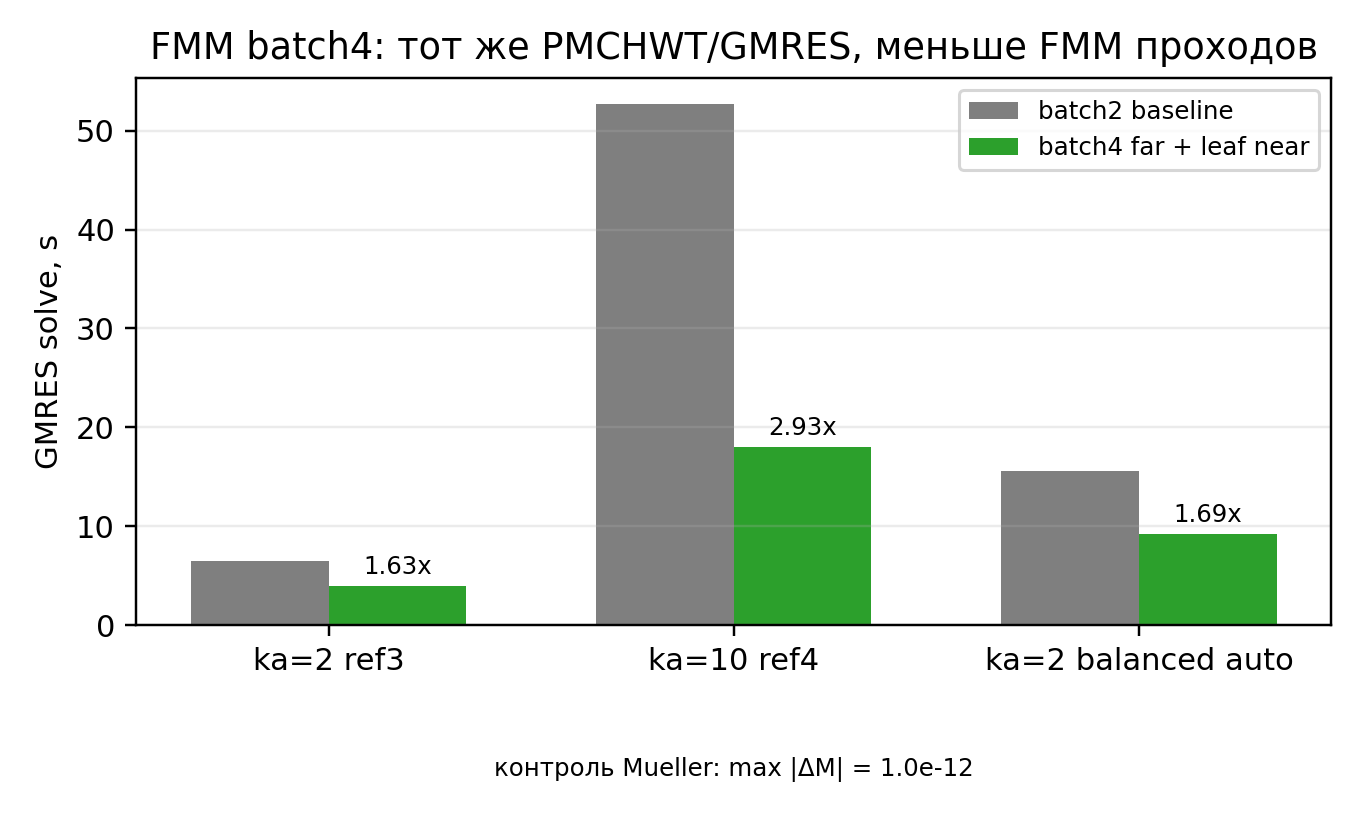
\includegraphics[width=0.96\textwidth]{fig_batch4_benchmark.png}
\caption{Эффект пакетного вычисления двух токов и двух поляризаций. Ускорение относится
к конкретной версии ядра и не заменяет контроль итоговой невязки.}
\label{fig:batch4}
\end{figure}

\chapter{Рекомендуемые профили}
\section{Предварительная диагностика}
Используется для проверки запуска и поиска грубых ошибок, но не для публикации:
\begin{lstlisting}[language=bash]
--solver fmm --quad 7 --fmm-digits 5 --gmres-tol 1e-3 \
--gmres-restart 300 --max-leaf 128 --no-prec
\end{lstlisting}

\section{Контролируемая несферическая частица}
\begin{lstlisting}[language=bash]
--accurate --solver fmm --system balanced --quad 7 \
--fmm-digits 7 --gmres-tol 1e-5 --gmres-restart 1000 \
--gmres-max-cycles 80 --max-leaf 128
\end{lstlisting}
Если программа усиливает параметры из-за mesh guard, в публикации указываются
эффективные значения из JSON, а не только исходная команда.

\section{Экспериментальные решатели}
\code{--krylov qmr2}, \code{cocr} и \code{block-cocg} предназначены для исследования.
На текущих тестах они не превзошли GPU-GMRES. Автоматический откат должен оставаться
включённым; отчёт обязан различать матвек-итерации предварительного решателя и GMRES.

\part{Форматы, диагностика и воспроизводимость}

\chapter{Выходной JSON}
JSON содержит физические параметры, описание сетки, запрошенную и фактическую систему,
backend, точность FMM, параметры GMRES, статистику сходимости, времена и массив
\code{mueller}. Перед объединением частей проверяются совместимость $ka$, $m$, $N_\theta$,
системы, сетки ориентаций и нормировки весов. Простое усреднение файлов с разными весами
неправильно.

Ключи \code{gmres\_converged\_systems}, \code{gmres\_max\_final\_relres} и
\code{accuracy\_policy\_adjusted} обязательны для аудита. Если отсутствует комплексный
масштаб строки или происхождение сетки, старый файл нельзя автоматически считать
эквивалентным новой версии.

\chapter{Диагностика типичных ошибок}
\section{Отрицательный $M_{11}$}
Физически недопустим. Проверяются индексы амплитудной матрицы, формулы Стокса,
комплексное сопряжение, веса ориентаций и повреждение JSON. Уменьшение GMRES tolerance
не является первым исправлением.

\section{Совпадение только в переднем направлении}
Проверяются интеграл $I_{11}$, нормировка размера OBJ, геометрия боковых граней,
квадратура близких панелей, поляризационная база и полнота ориентационной сетки.
Передний пик может совпадать при существенной потере энергии в задней полусфере.

\section{Сетка мельче, а ошибка не уменьшается}
Возможны: неизменившаяся геометрическая аппроксимация, недостаточная квадратура,
достигнутый предел FMM/GMRES, плохие треугольники или сравнение разных ориентаций.
Изменять одновременно ref, quad, digits и tol нельзя: причина станет неидентифицируемой.

\section{Процесс завис около допуска}
Короткая рекуррентность может иметь ложную рекурсивную невязку. Используется истинный
пересчёт $b-Ax$, ограничение стагнации, сохранение лучшего решения и откат на GMRES.
Файл без финального Mueller при нулевой загрузке GPU считается аварийно незавершённым.

\chapter{Воспроизводимый вычислительный эксперимент}
Для каждой точки сохраняются:
\begin{itemize}
\item commit Git и контрольная сумма бинарного файла;
\item полная команда и значимые переменные окружения;
\item GPU, драйвер CUDA и лимит мощности;
\item исходная сетка и её отчёт качества;
\item JSON, stdout/stderr и время;
\item скрипт сравнения и эталонные данные;
\item критерий принятия до запуска, а не после просмотра графика.
\end{itemize}
Нельзя подгонять масштаб кривой или выбор углов после расчёта и затем называть результат
прямым сравнением. Любое преобразование нормировки должно быть записано формулой.

\appendix
\part{Справочные приложения}

\chapter{Справочник основных параметров CLI}
\begin{longtable}{p{0.28\textwidth}p{0.64\textwidth}}
\toprule Параметр & Назначение и рекомендация\\\midrule
\code{--ka F} & Размерный параметр $ka_{\rm eq}$; обязателен.\\
\code{--ri RE IM} & Комплексный показатель $m=\mathrm{RE}+\iu\mathrm{IM}$.\\
\code{--shape sphere|hex\_prism} & Встроенная геометрия.\\
\code{--obj FILE} & Замкнутая триангулированная поверхность, нормируемая по объёму.\\
\code{--ref N} & Уровень икосферической сетки.\\
\code{--prism-aspect F} & Отношение сторон призмы в соглашении ADDA.\\
\code{--quad 4|7|13} & Порядок треугольной квадратуры.\\
\code{--solver auto|dense|fmm|pfft|spfft} & Backend; рабочий большой расчёт использует FMM.\\
\code{--system balanced} & Рекомендуемая масштабированная PMCHWT-система.\\
\code{--fmm-digits N} & Точность дальнего FMM-взаимодействия, обычно 6--8.\\
\code{--max-leaf N} & Максимум источников/частиц листа, обычно 128.\\
\code{--gmres-tol F} & Истинная относительная невязка; строгий OBJ обычно $10^{-5}$.\\
\code{--gmres-restart N} & Размер пространства до перезапуска; влияет на память.\\
\code{--gmres-max-cycles N} & Максимум циклов перезапуска.\\
\code{--krylov gmres} & Основной решатель; другие значения экспериментальны.\\
\code{--single} & Одна ориентация без усреднения.\\
\code{--orient NA NB NG} & Явная сетка углов Эйлера.\\
\code{--orient-file FILE} & Явные углы и веса.\\
\code{--orient-bg-file FILE} & Сетка $\beta,\gamma$ для ускоренного $\alpha$-усреднения.\\
\code{--alpha-avg N} & Число дешёвых узлов по $\alpha$.\\
\code{--orient-start/--orient-count} & Разбиение ориентаций на возобновляемые части.\\
\code{--ntheta N} & Число углов рассеяния от 0 до $180^\circ$.\\
\code{--scat-plane yz|xz} & Плоскость рассеяния одной ориентации.\\
\code{--accurate} & Усиливает контролируемые настройки несферических частиц.\\
\code{--fast-obj} & Старый быстрый профиль; только диагностика.\\
\code{--mesh-quality-only} & Проверка поверхности без решения.\\
\code{--mesh-quality-strict} & Остановка при непрохождении gate.\\
\code{--export-currents FILE} & Экспорт токов VTK для одной ориентации.\\
\code{--out FILE} & Итоговый JSON.\\\bottomrule
\end{longtable}

\chapter{Классы переменных окружения}
В коде присутствует большое число диагностических переменных \code{BEM\_*}. Они не
являются стабильным пользовательским API. Основные классы:
\begin{description}
\item[Устройство.] Выбор GPU, пакетных ядер и pinned staging.
\item[FMM.] Кэш M2L, размер рабочих слотов, локальные коррекции и аудит дерева.
\item[GMRES/Krylov.] GPU-путь, частота истинной невязки, критерии стагнации и fallback.
\item[Предобуславливатель.] Размер локального блока, ближний граф, число проходов.
\item[Ориентации.] Пакет дальнего поля, аналитическое $\alpha$-усреднение, split output.
\item[Аудит.] Проверка симметрии, коэффициентов, памяти и качества результата.
\end{description}
Перед публикацией переменные окружения записываются вместе с командой. Неописанная
переменная из экспериментального скрипта не должна переноситься в производственный
профиль без отдельного A/B-теста.

\chapter{Формат файлов ориентаций}
\section{Полная сетка}
\begin{Verbatim}[frame=single]
# alpha_deg beta_deg gamma_deg weight
0.0  35.2643897  0.0  0.0833333333
90.0 35.2643897  0.0  0.0833333333
\end{Verbatim}
Сумма весов может быть произвольной, если объединяющий код явно нормирует её. Для
частичных файлов сохраняется глобальный индекс ориентации.

\section{Фоновая сетка $\beta,\gamma$}
\begin{Verbatim}[frame=single]
# beta_deg gamma_deg weight
35.2643897 0.0 0.25
90.0       0.0 0.50
144.7356103 0.0 0.25
\end{Verbatim}
Она используется совместно с \code{--alpha-avg}. Нельзя сравнивать результат с ADDA,
если фактические узлы и веса ADDA неизвестны.

\chapter{Контрольный лист публикационного расчёта}
\begin{enumerate}[label=\arabic*.]
\item Геометрия замкнута, ориентирована наружу, отчёт качества сохранён.
\item $ka$ определён через эквивалентный объём и совпадает с эталоном.
\item Материал и знак мнимой части согласованы с $e^{-\iu\omega t}$.
\item Плотный и FMM-пути совпадают на уменьшенной сетке.
\item Два уровня поверхности дают изменение меньше целевой ошибки.
\item $q=7$ и $q=13$ проверены хотя бы на наиболее сложном размере.
\item digits увеличен на единицу без значимого изменения результата.
\item Истинная невязка ниже выбранного допуска для обеих поляризаций.
\item Интеграл $M_{11}$ стабилен; $M_{11}\ge0$.
\item Ориентационное усреднение сошлось минимум на двух вложенных сетках.
\item Сравнение использует одинаковые ориентации и поляризационную базу.
\item Время приведено на одну указанную GPU и включает явно перечисленные этапы.
\item Память является измеренной, прогнозы отмечены как прогнозы.
\item Все не сошедшиеся точки исключены, а не скрыты масштабированием.
\item Сохранены commit, команда, окружение, JSON, логи и исходная сетка.
\end{enumerate}

\chapter{Происхождение включённых графиков}
Все рисунки этого руководства взяты из каталога \code{poster\_a0/assets} текущего
рабочего дерева. Их машинно-читаемые источники находятся рядом:
\begin{longtable}{p{0.38\textwidth}p{0.54\textwidth}}
\toprule Рисунок & Таблица/назначение\\\midrule
\code{fig\_mie\_validation\_combined.png} & \code{table\_mie\_validation.csv}, контроль Ми.\\
\code{fig\_dust\_fullgrid\_compare.png} & \code{table\_dust\_fullgrid\_compare.csv}, BEM--ADDA.\\
\code{fig\_vram\_forecast.png} & \code{table\_vram\_experiment.csv} и прогнозная таблица.\\
\code{fig\_shape\_single\_time.png} & \code{table\_shape\_single\_time.csv}.\\
\code{fig\_orientation\_convergence.png} & данные вложенных ориентационных сеток.\\
\code{fig\_batch4\_benchmark.png} & \code{table\_batch4\_benchmark.csv}.\\
\bottomrule
\end{longtable}
Перед повторным использованием следует проверить \code{table\_figure\_provenance.csv}
и свежесть результата относительно commit программы.

\chapter{Атлас численных экспериментов}
Этот атлас предназначен не для декоративного увеличения документа, а для фиксации
типичных способов контроля. Каждый рисунок должен рассматриваться вместе с исходной
таблицей и метаданными расчёта. Кривые из разных экспериментов нельзя объединять без
проверки геометрии, материала, ориентаций и нормировки.

\clearpage
\section{Зависимость от показателя преломления}
\begin{figure}[H]\centering
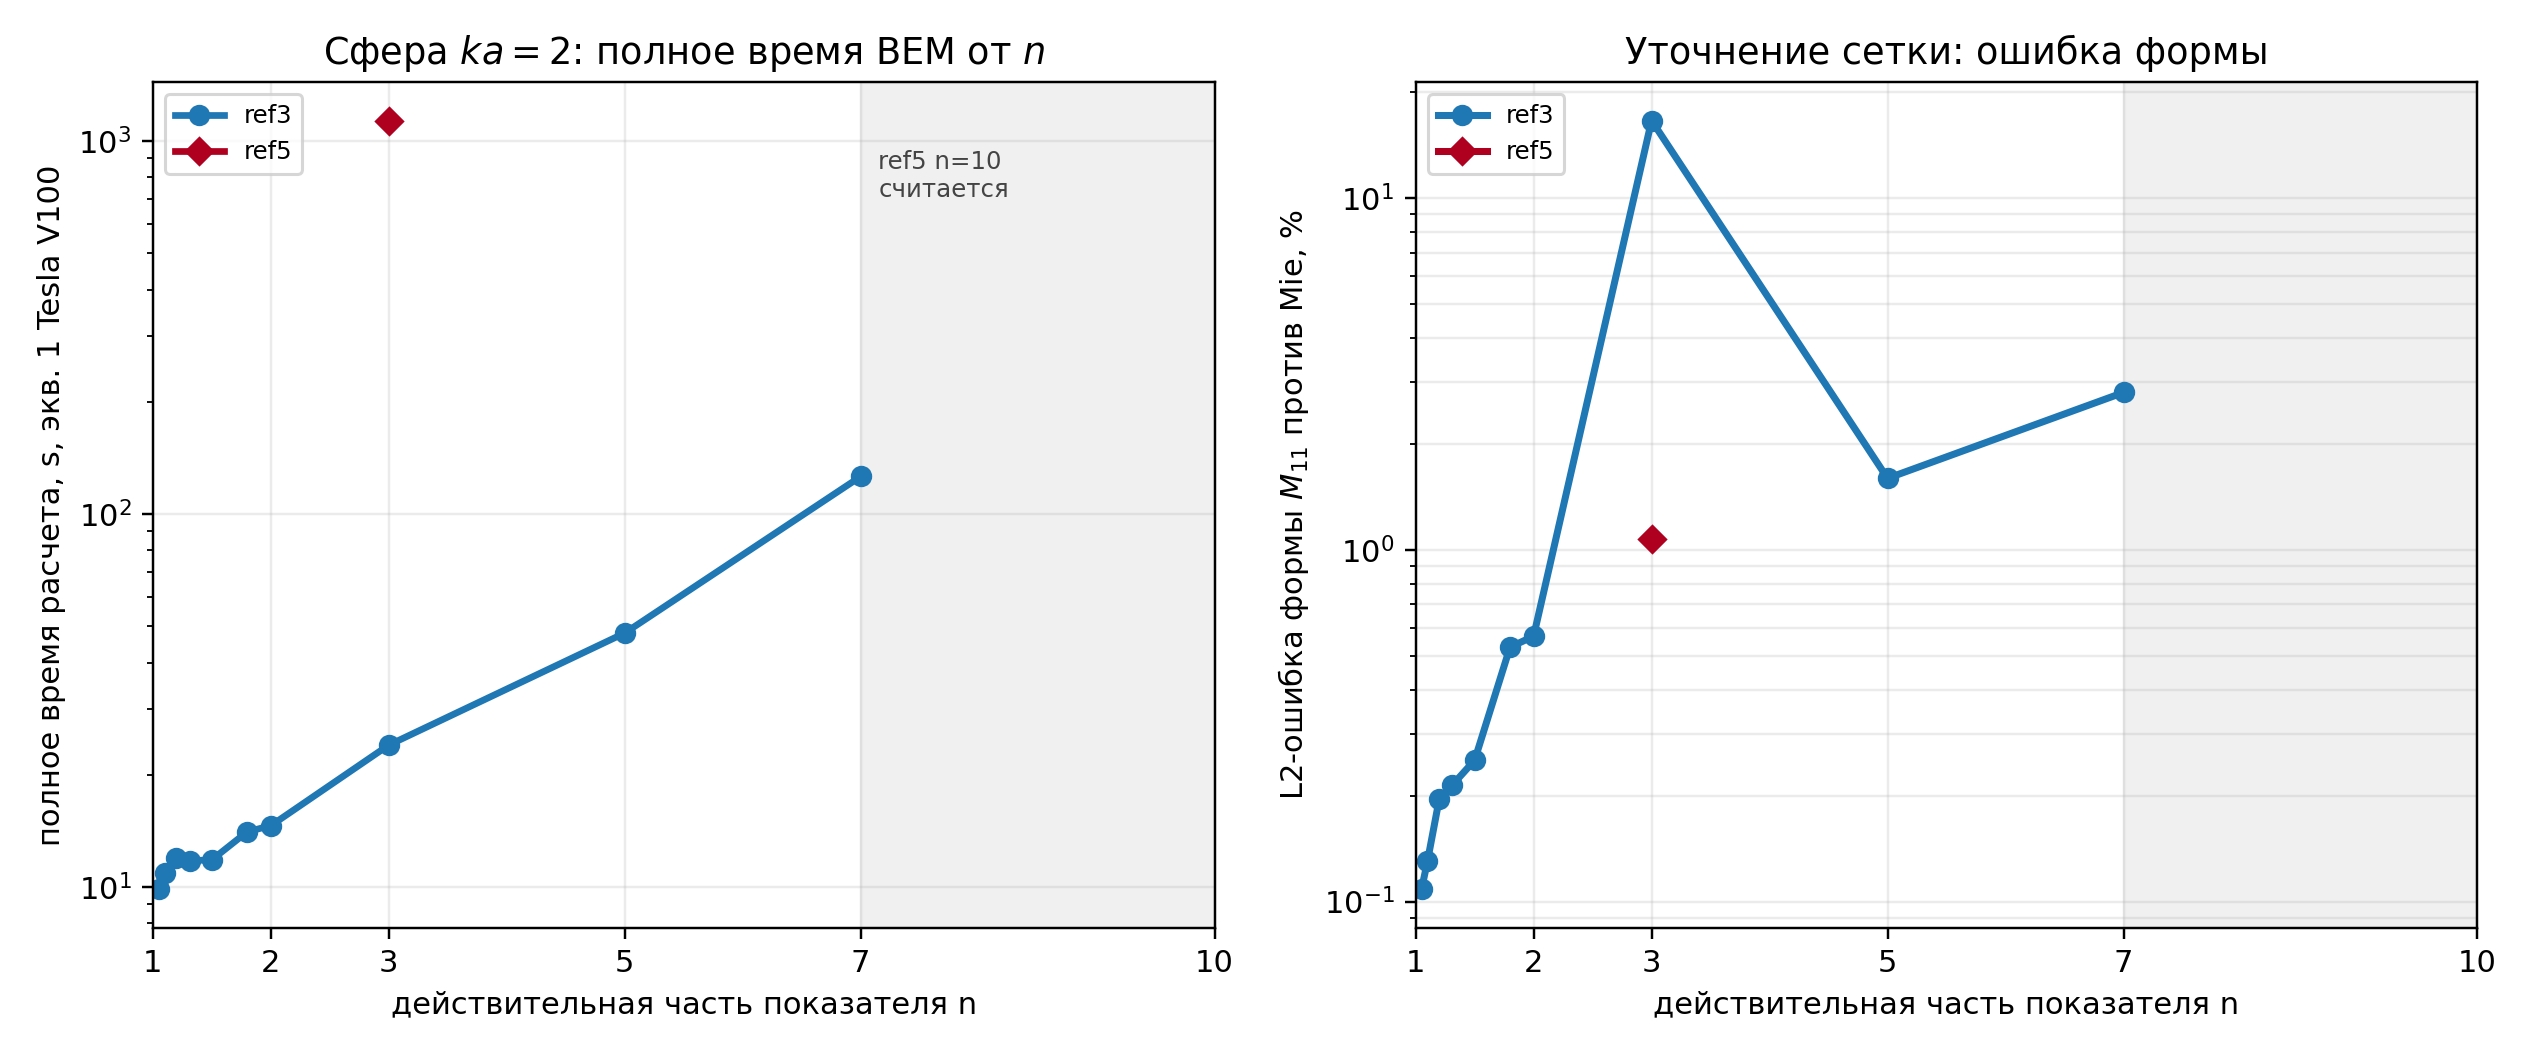
\includegraphics[width=0.96\textwidth,height=0.78\textheight,keepaspectratio]{fig_index_sweep.png}
\caption{Серия расчётов по показателю преломления. Рост $|m|$ обычно ухудшает
обусловленность и повышает требования к сетке; отдельная точка не задаёт универсальный
закон времени.}\end{figure}
Перед интерпретацией следует проверить, что каждая точка прошла одинаковый критерий
невязки и сеточной сходимости. Уменьшение времени при большем $m$ может быть следствием
досрочной несходимости, а не ускорения метода.

\clearpage
\section{Строгий контроль сферы}
\begin{figure}[H]\centering
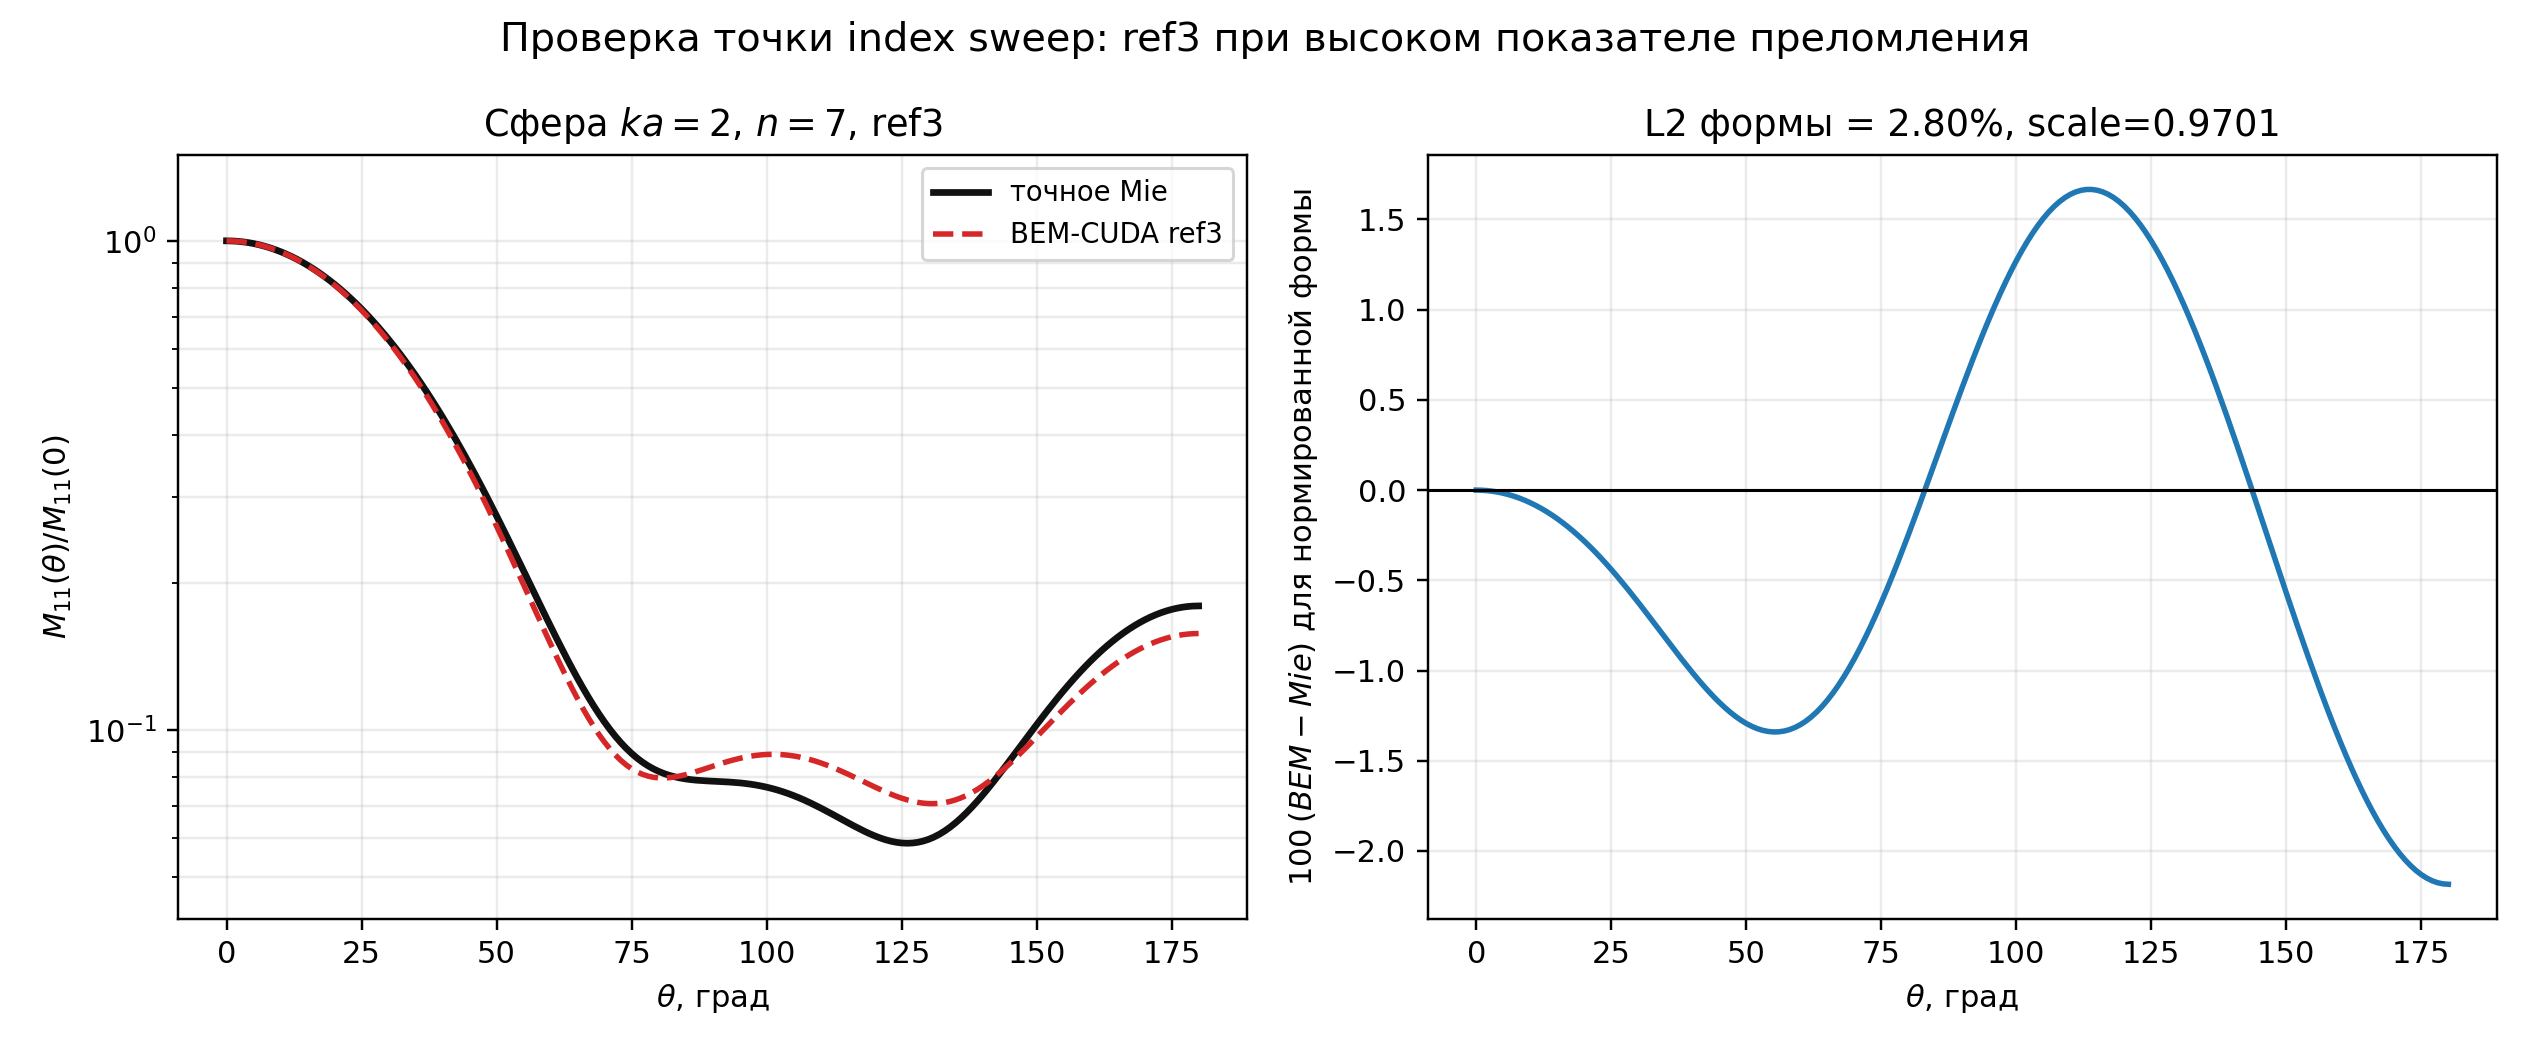
\includegraphics[width=0.96\textwidth,height=0.78\textheight,keepaspectratio]{fig_mie_n7_ref3_compare.png}
\caption{Покомпонентное сравнение BEM и Ми при фиксированной сетке. Фазовая функция
и нормированные элементы требуют разных шкал.}\end{figure}
Сфера выявляет ошибки поляризационной базы, которые могут быть незаметны по одному
$M_{11}$. В отчёте указывается не только средняя ошибка, но и максимальная ошибка
сильных элементов и интеграл фазовой функции.

\clearpage
\section{Необработанное сравнение с ADDA}
\begin{figure}[H]\centering
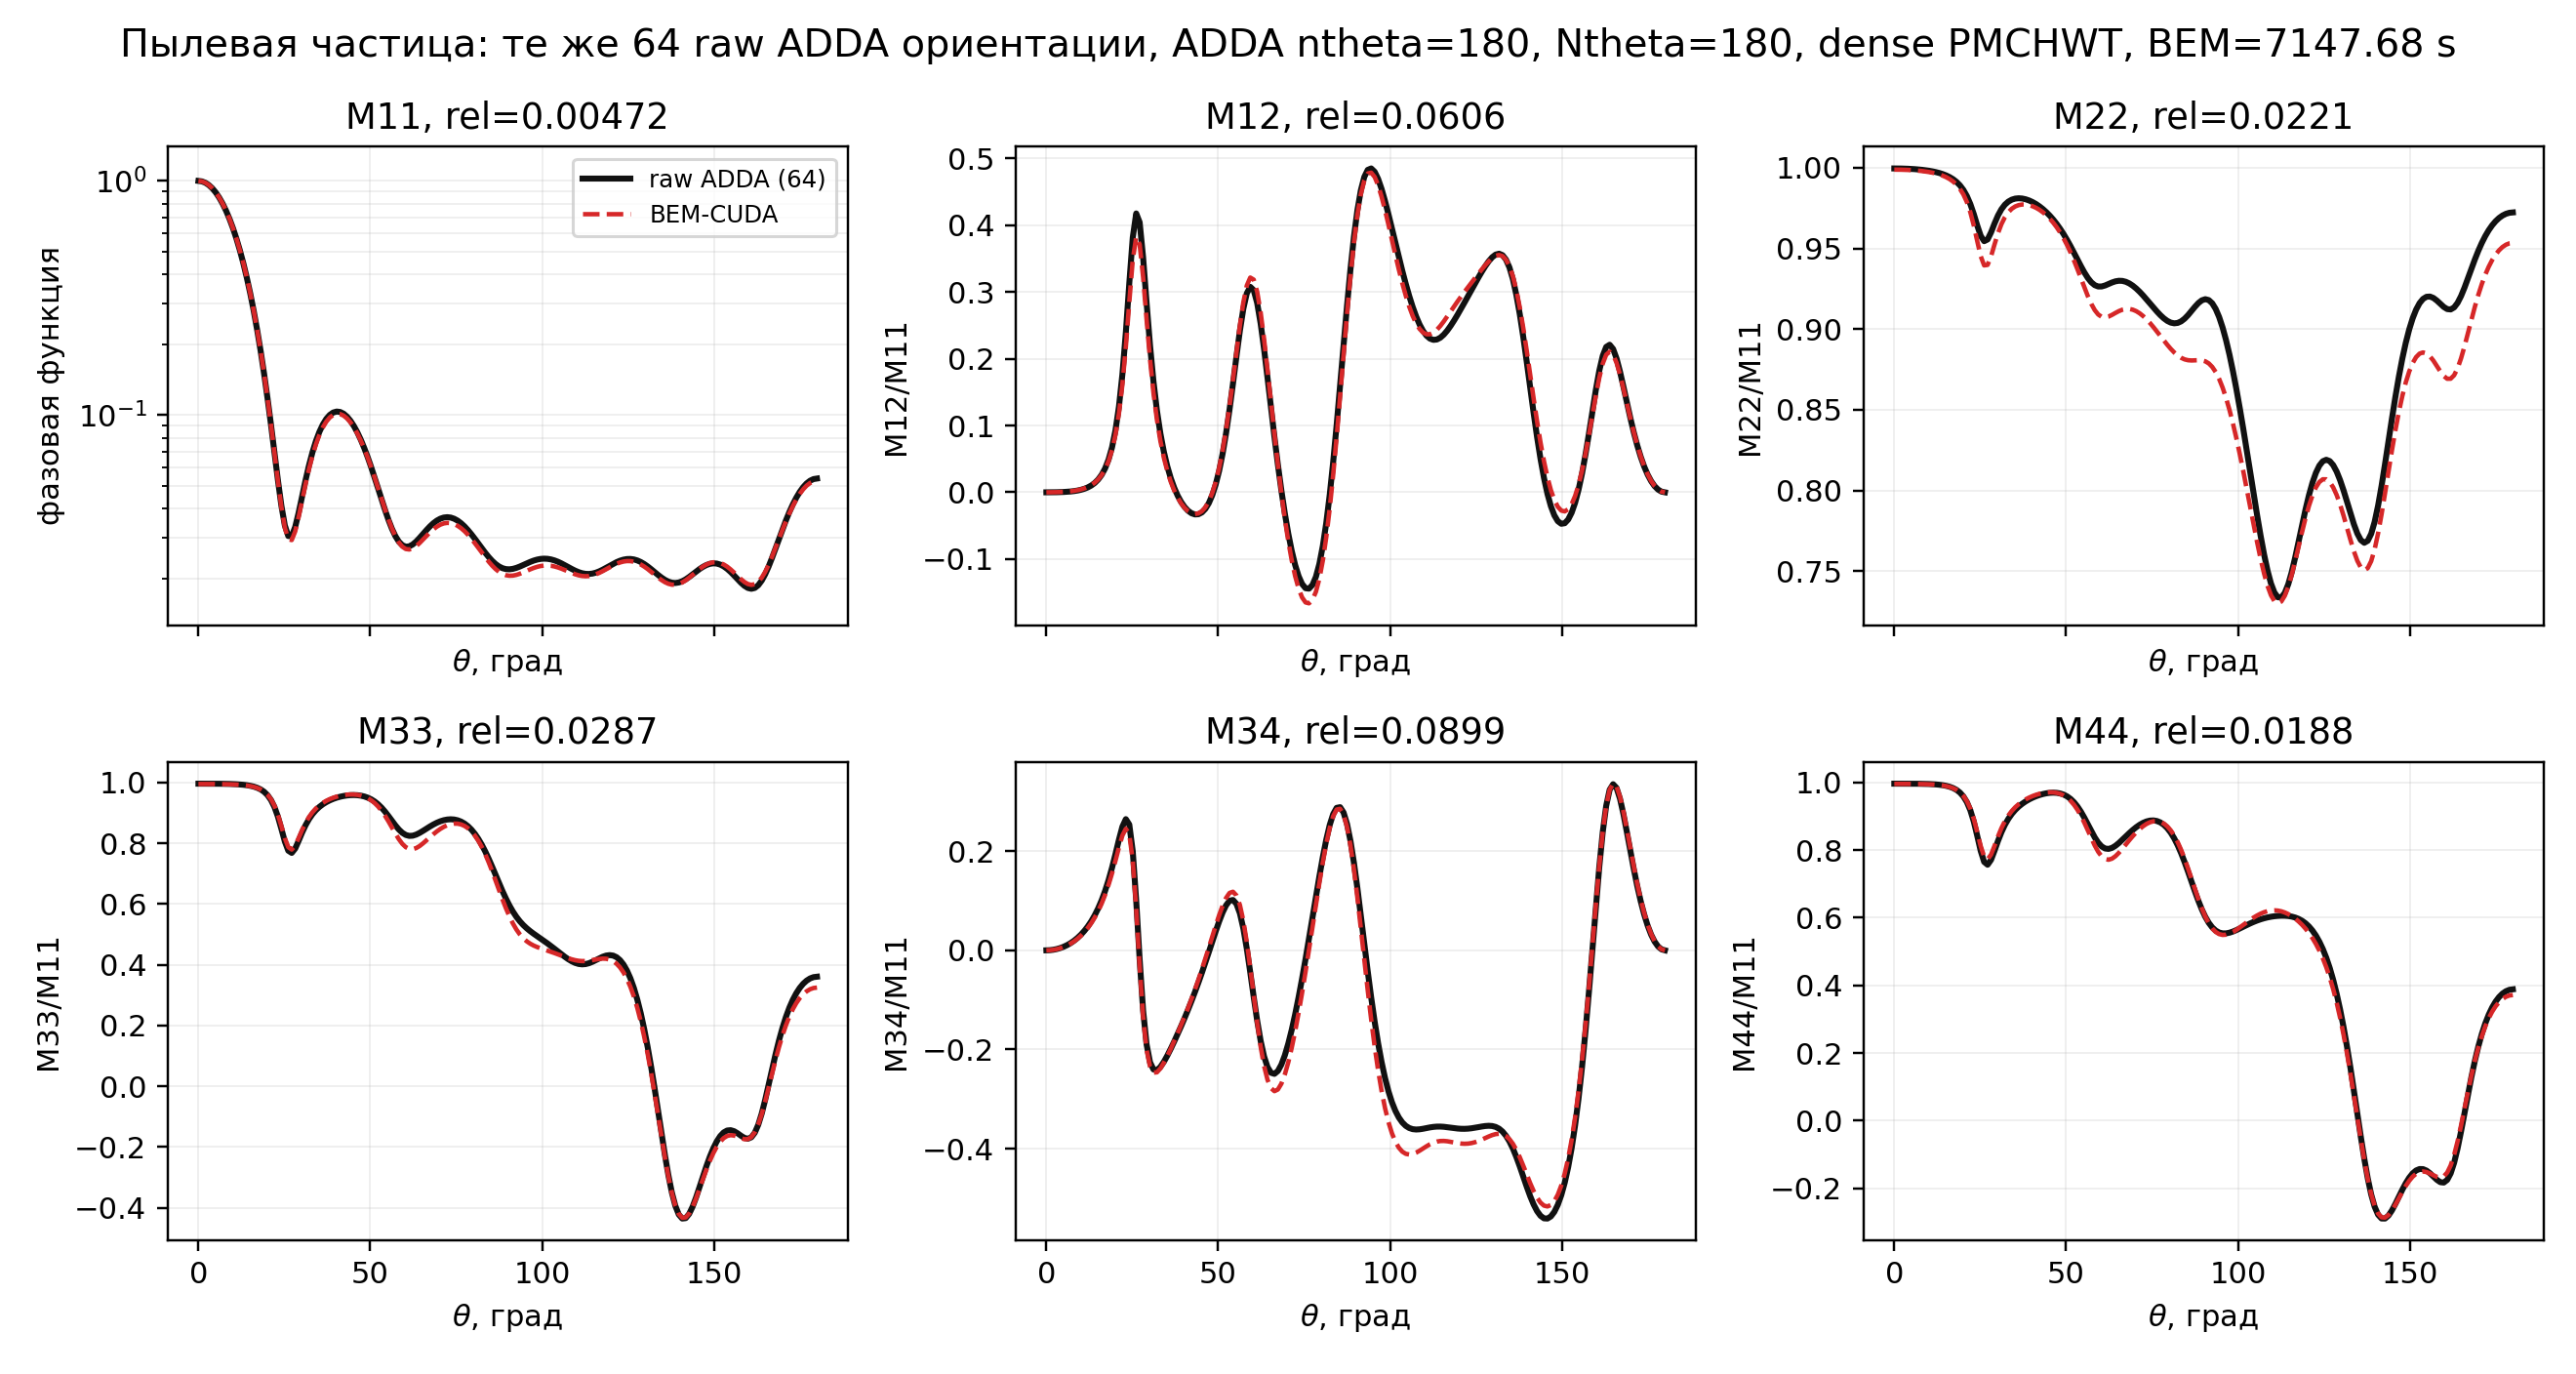
\includegraphics[width=0.96\textwidth,height=0.77\textheight,keepaspectratio]{fig_dust_raw_adda_compare.png}
\caption{Сравнение исходных данных BEM и ADDA без искусственного масштабирования.}
\end{figure}
Такой график должен строиться первым. Масштабирование одной кривой для визуального
совпадения допустимо только как отдельная диагностика нормировки и не является
результатом физического сравнения.

\clearpage
\section{Диагностика общей нормировки}
\begin{figure}[H]\centering
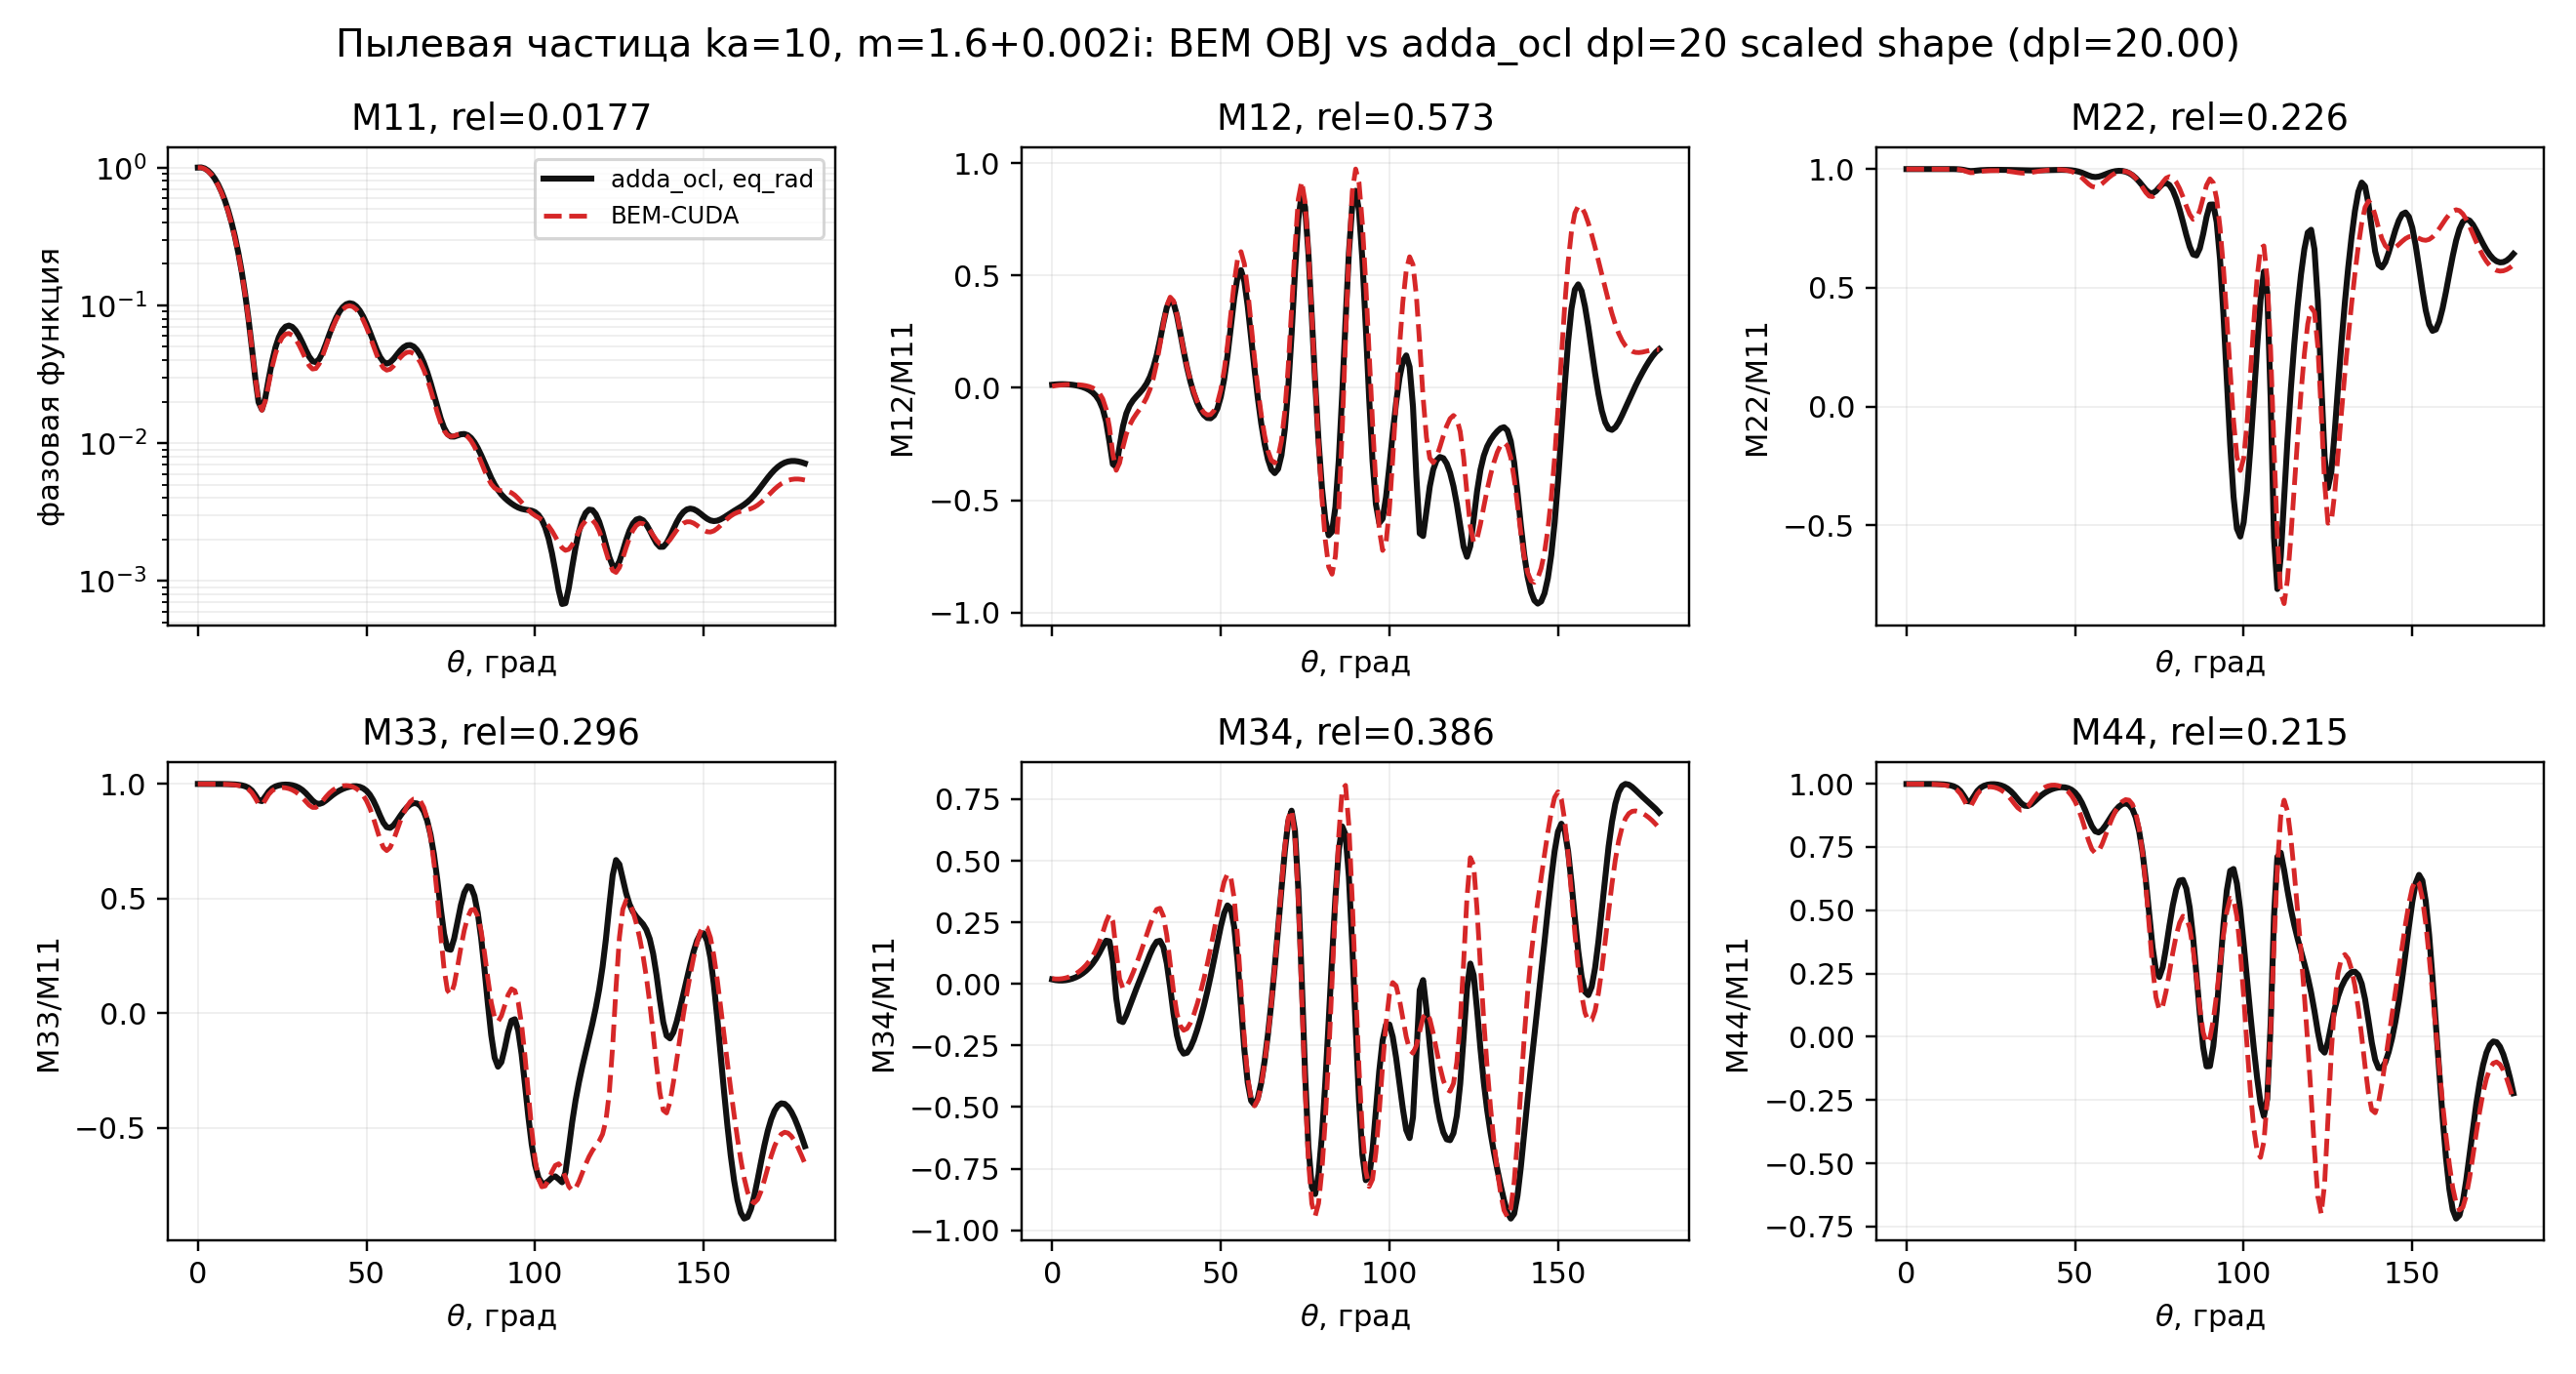
\includegraphics[width=0.96\textwidth,height=0.77\textheight,keepaspectratio]{fig_dust_ka10_adda_scaled.png}
\caption{Диагностическое масштабирование сравнения на пылевой частице.}
\end{figure}
Если один коэффициент улучшает все углы и элементы, проверяется нормировка амплитуды.
Если коэффициент помогает только переднему пику, причина, вероятнее всего, в геометрии
или угловом разрешении. Итоговые данные всегда возвращаются к физической нормировке.

\clearpage
\section{Слабые компоненты}
\begin{figure}[H]\centering
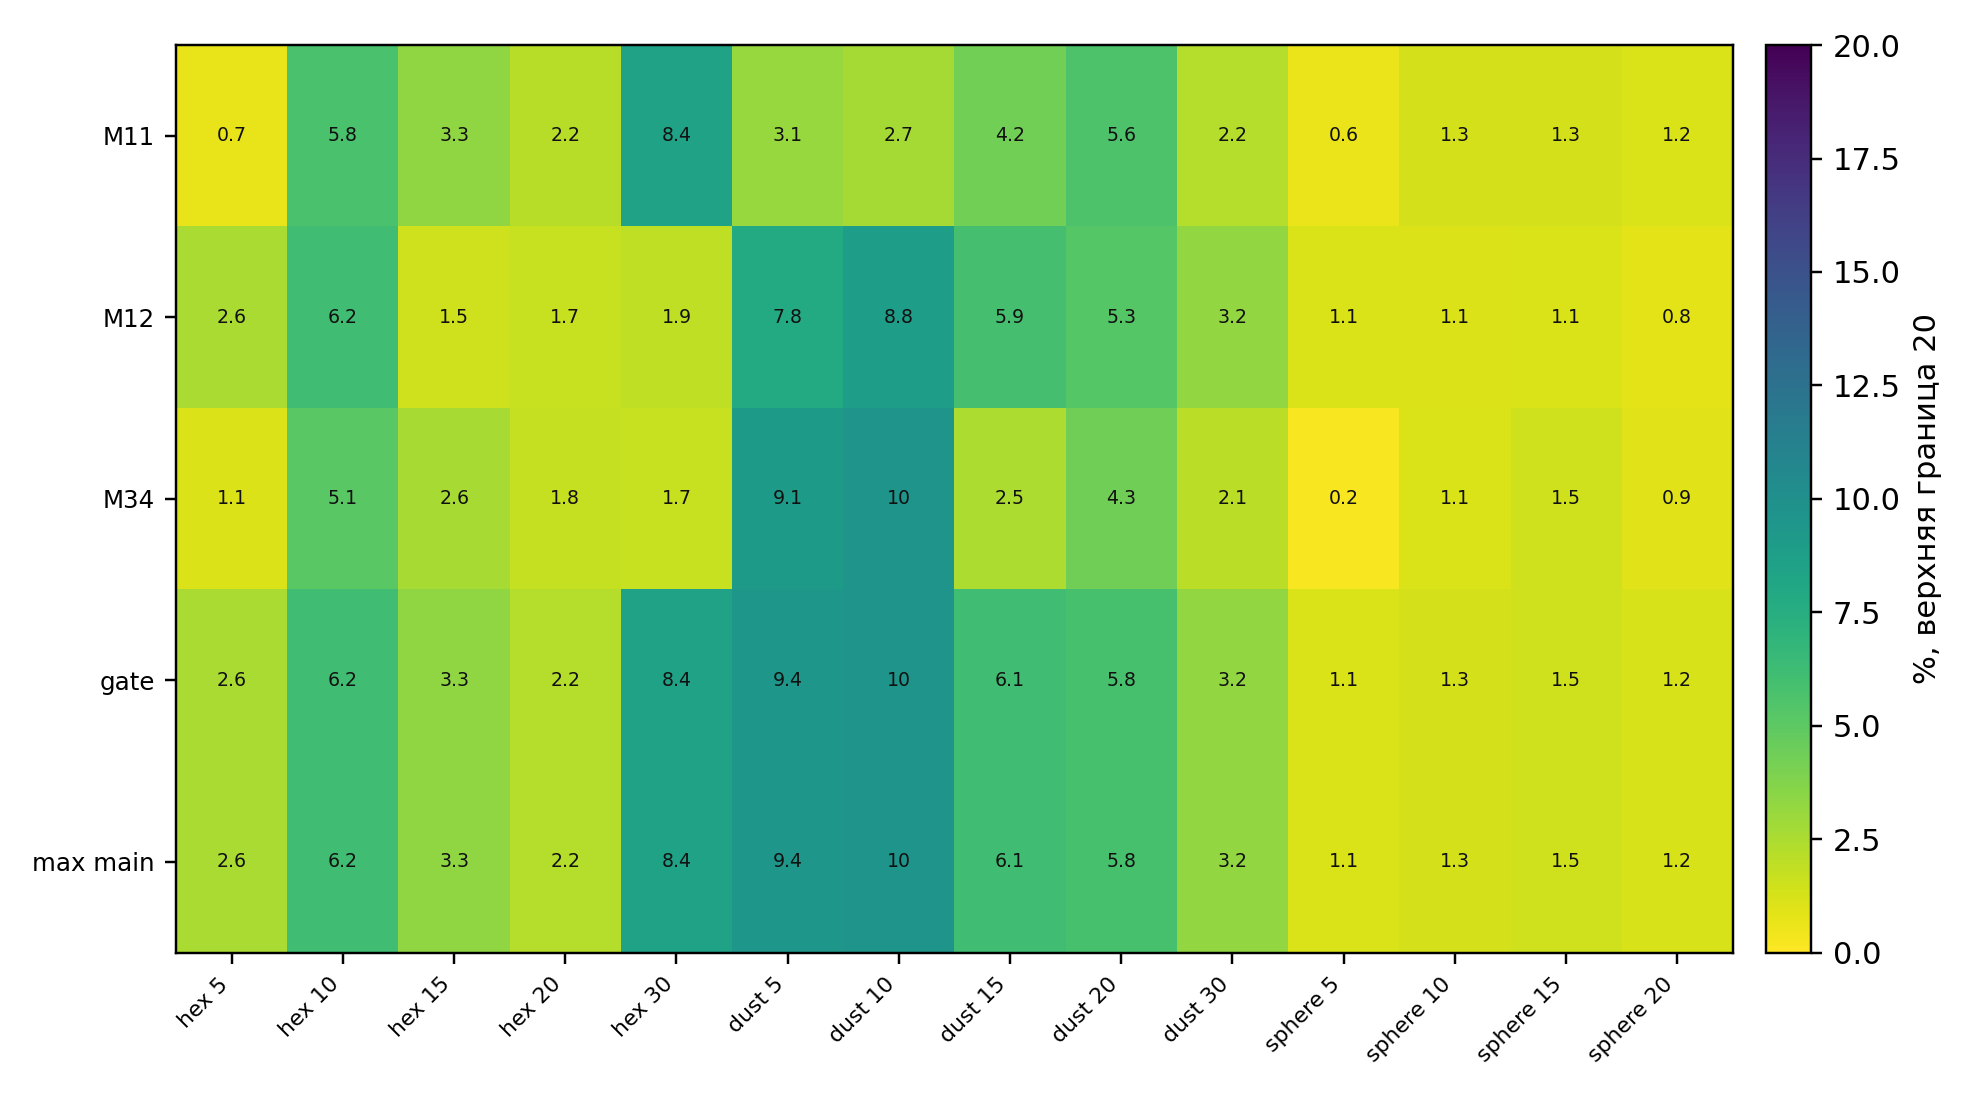
\includegraphics[width=0.96\textwidth,height=0.77\textheight,keepaspectratio]{fig_weak_component_metric.png}
\caption{Метрика слабых элементов матрицы Мюллера.}\end{figure}
Относительная ошибка около нуля неограниченно растёт, поэтому слабые элементы
нормируются на устойчивый масштаб, например интеграл $M_{11}$. Сильные и слабые
компоненты должны иметь раздельные критерии принятия.

\clearpage
\section{Точность гексагональной призмы}
\begin{figure}[H]\centering
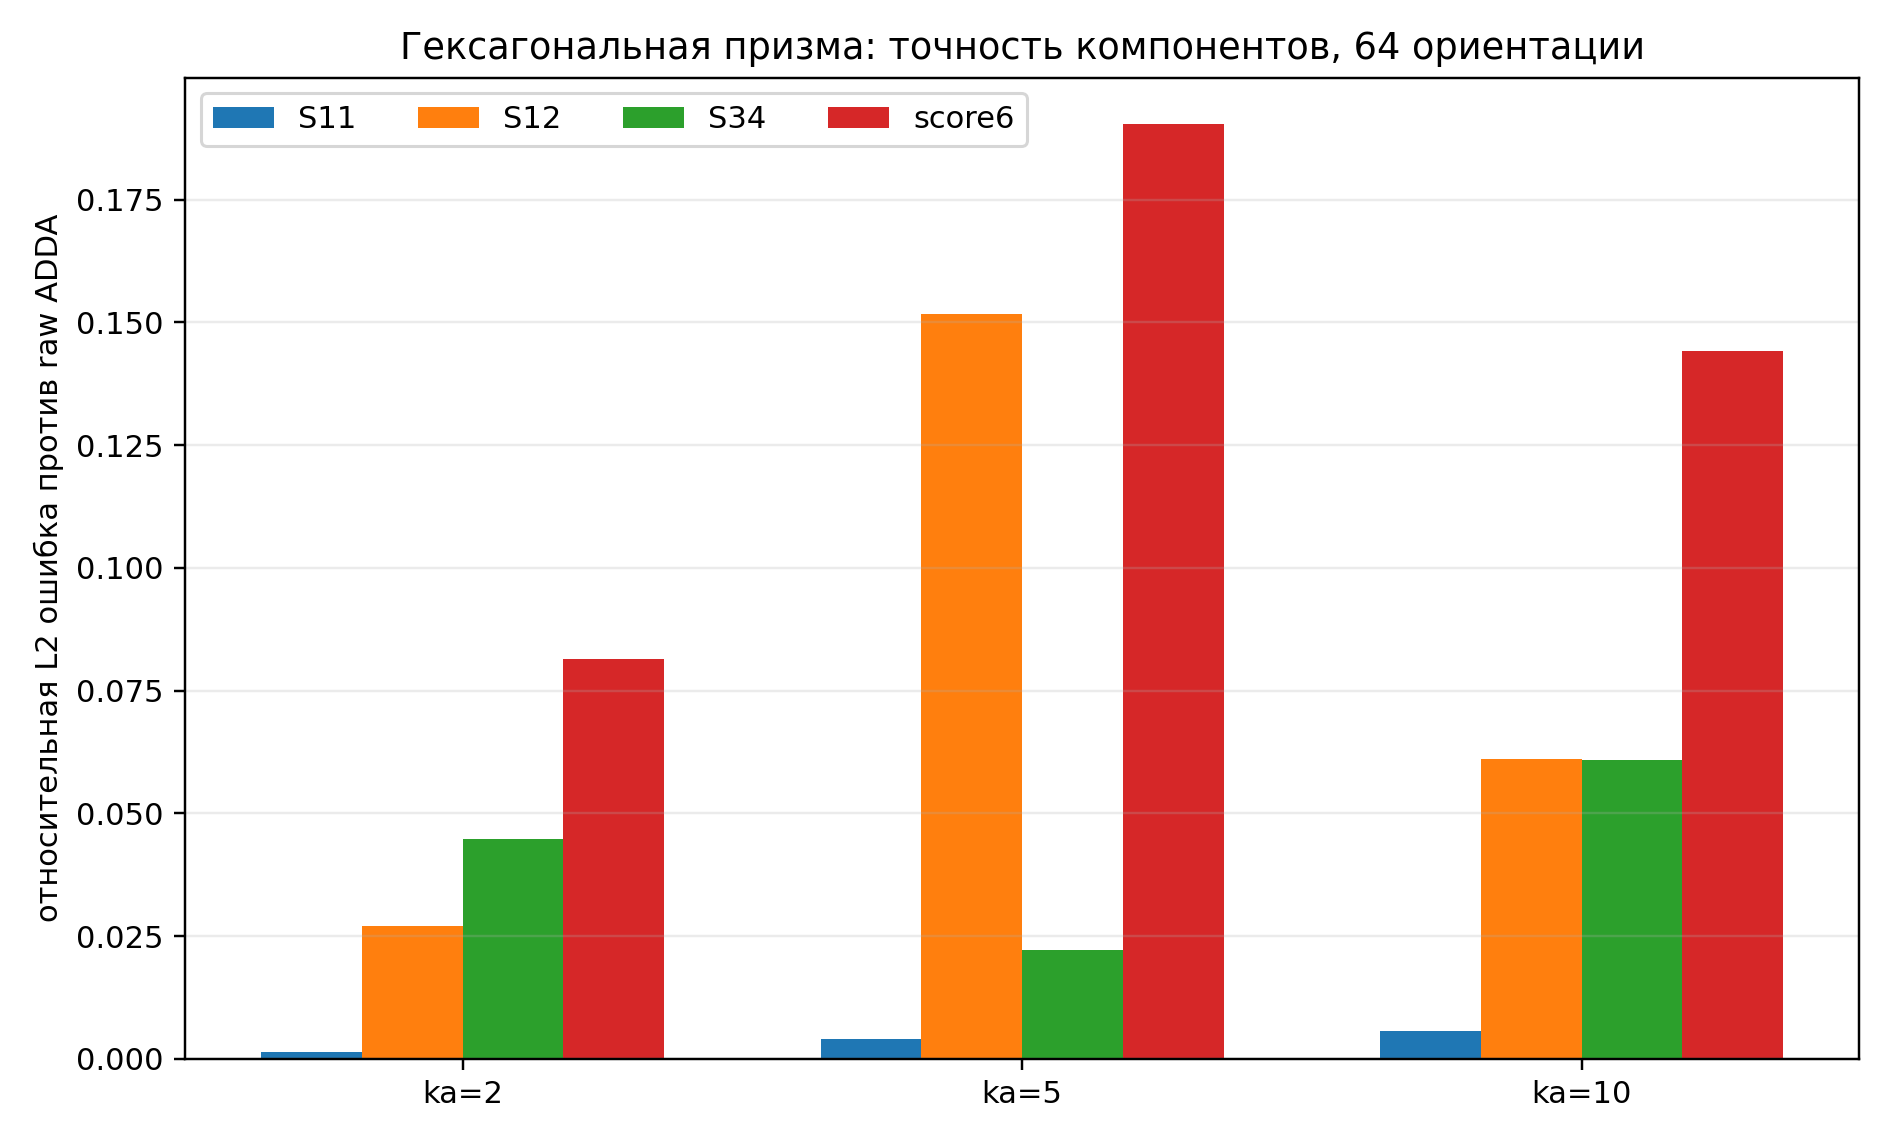
\includegraphics[width=0.96\textwidth,height=0.76\textheight,keepaspectratio]{fig_hex_accuracy.png}
\caption{Контроль точности для гексагональной призмы.}\end{figure}
Рёбра призмы создают особенности поверхностных токов. Поэтому одинаковое среднее
отношение длины волны к ребру не гарантирует одинаковую ошибку сферы и призмы.

\clearpage
\section{Скорость на призме}
\begin{figure}[H]\centering
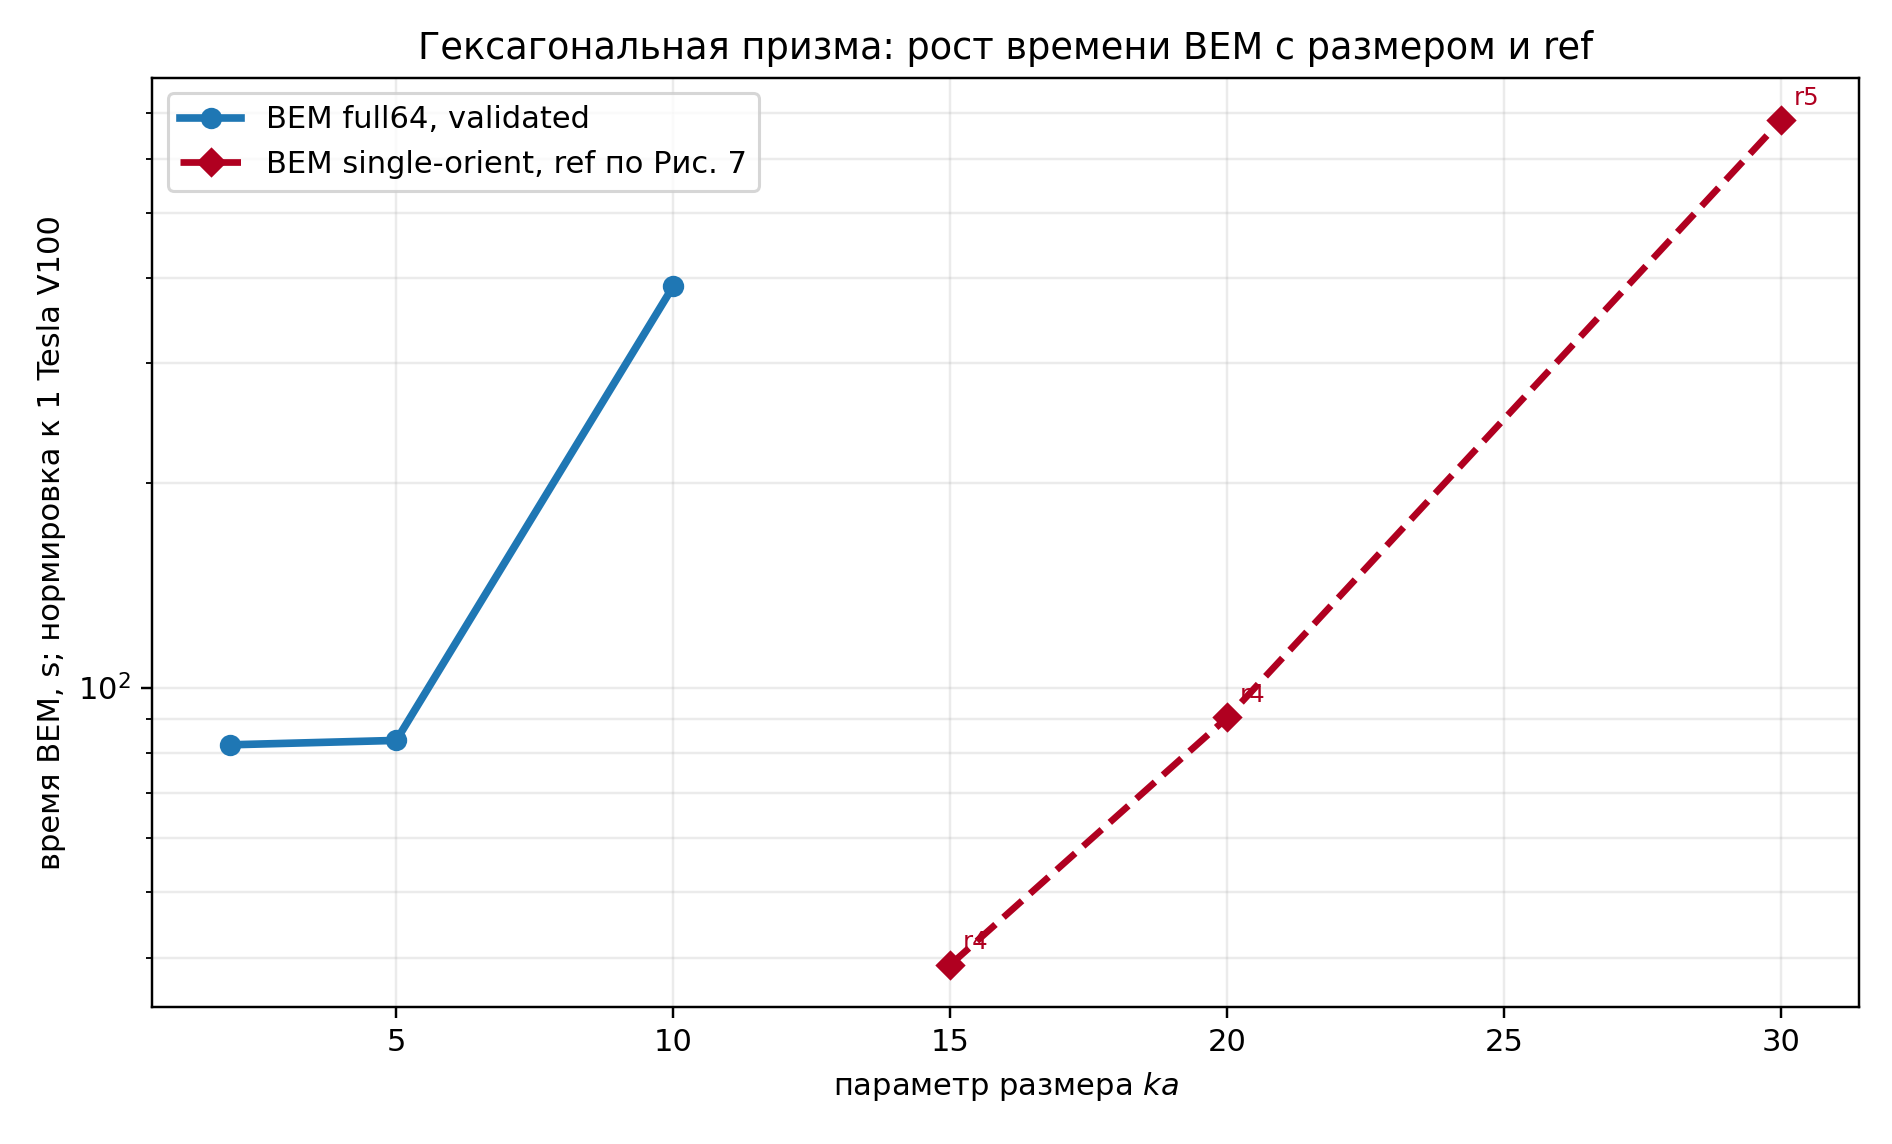
\includegraphics[width=0.96\textwidth,height=0.76\textheight,keepaspectratio]{fig_hex_speed.png}
\caption{Измеренное время расчёта призмы.}\end{figure}
График скорости имеет смысл только для точек, прошедших заданный критерий точности.
Не сошедшийся быстрый запуск отмечается отдельно и не соединяется производственной
линией.

\clearpage
\section{Обычный предобуславливатель}
\begin{figure}[H]\centering
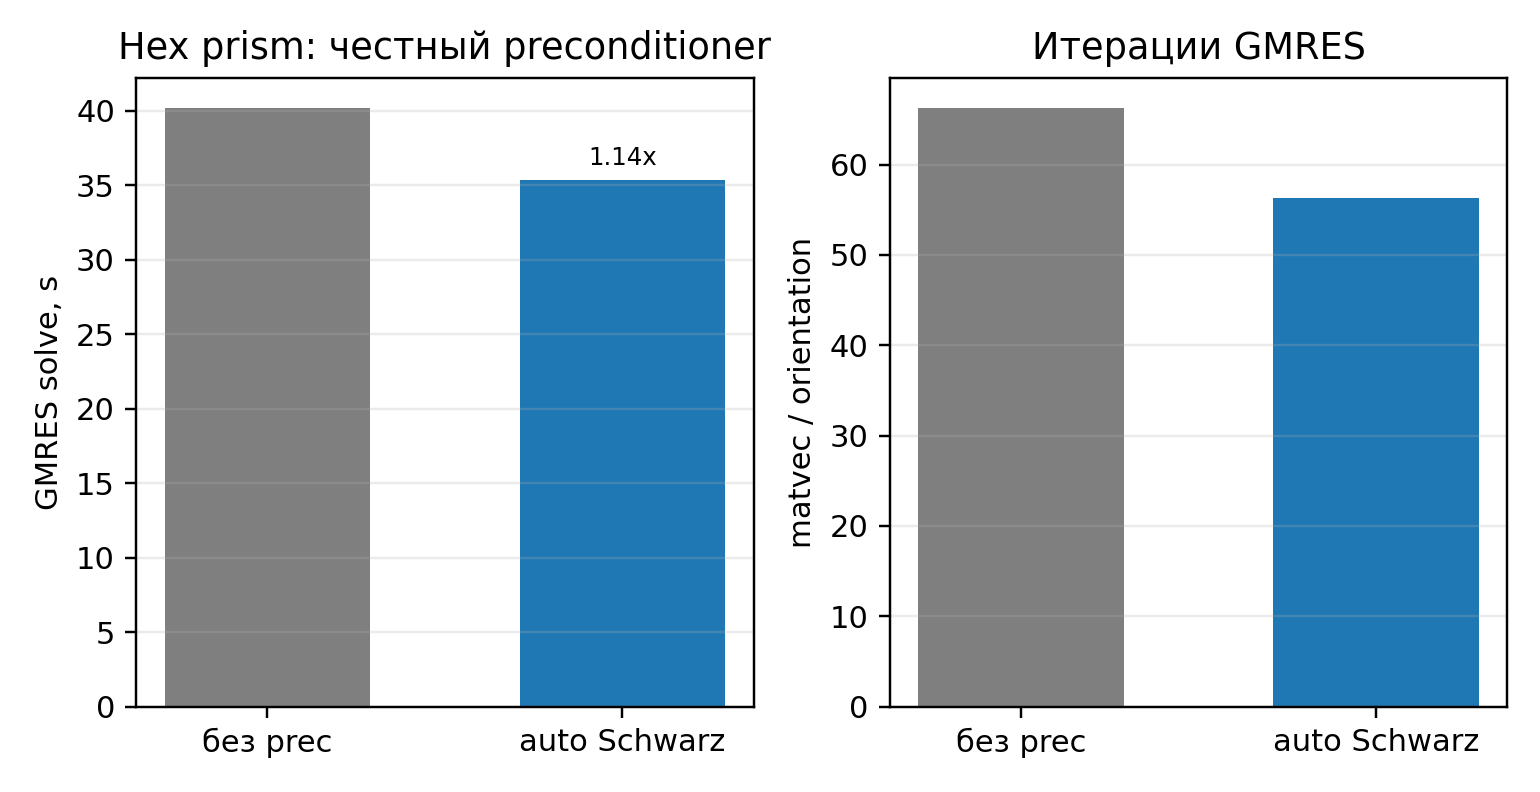
\includegraphics[width=0.96\textwidth,height=0.76\textheight,keepaspectratio]{fig_hex_precond_benchmark.png}
\caption{A/B-тест предобуславливателя на призме.}\end{figure}
Сравниваются полное время, число матвеков, стоимость построения и истинная невязка.
Снижение числа итераций не гарантирует снижение времени, если построение локальных
блоков доминирует.

\clearpage
\section{Сравнение backend-ов}
\begin{figure}[H]\centering
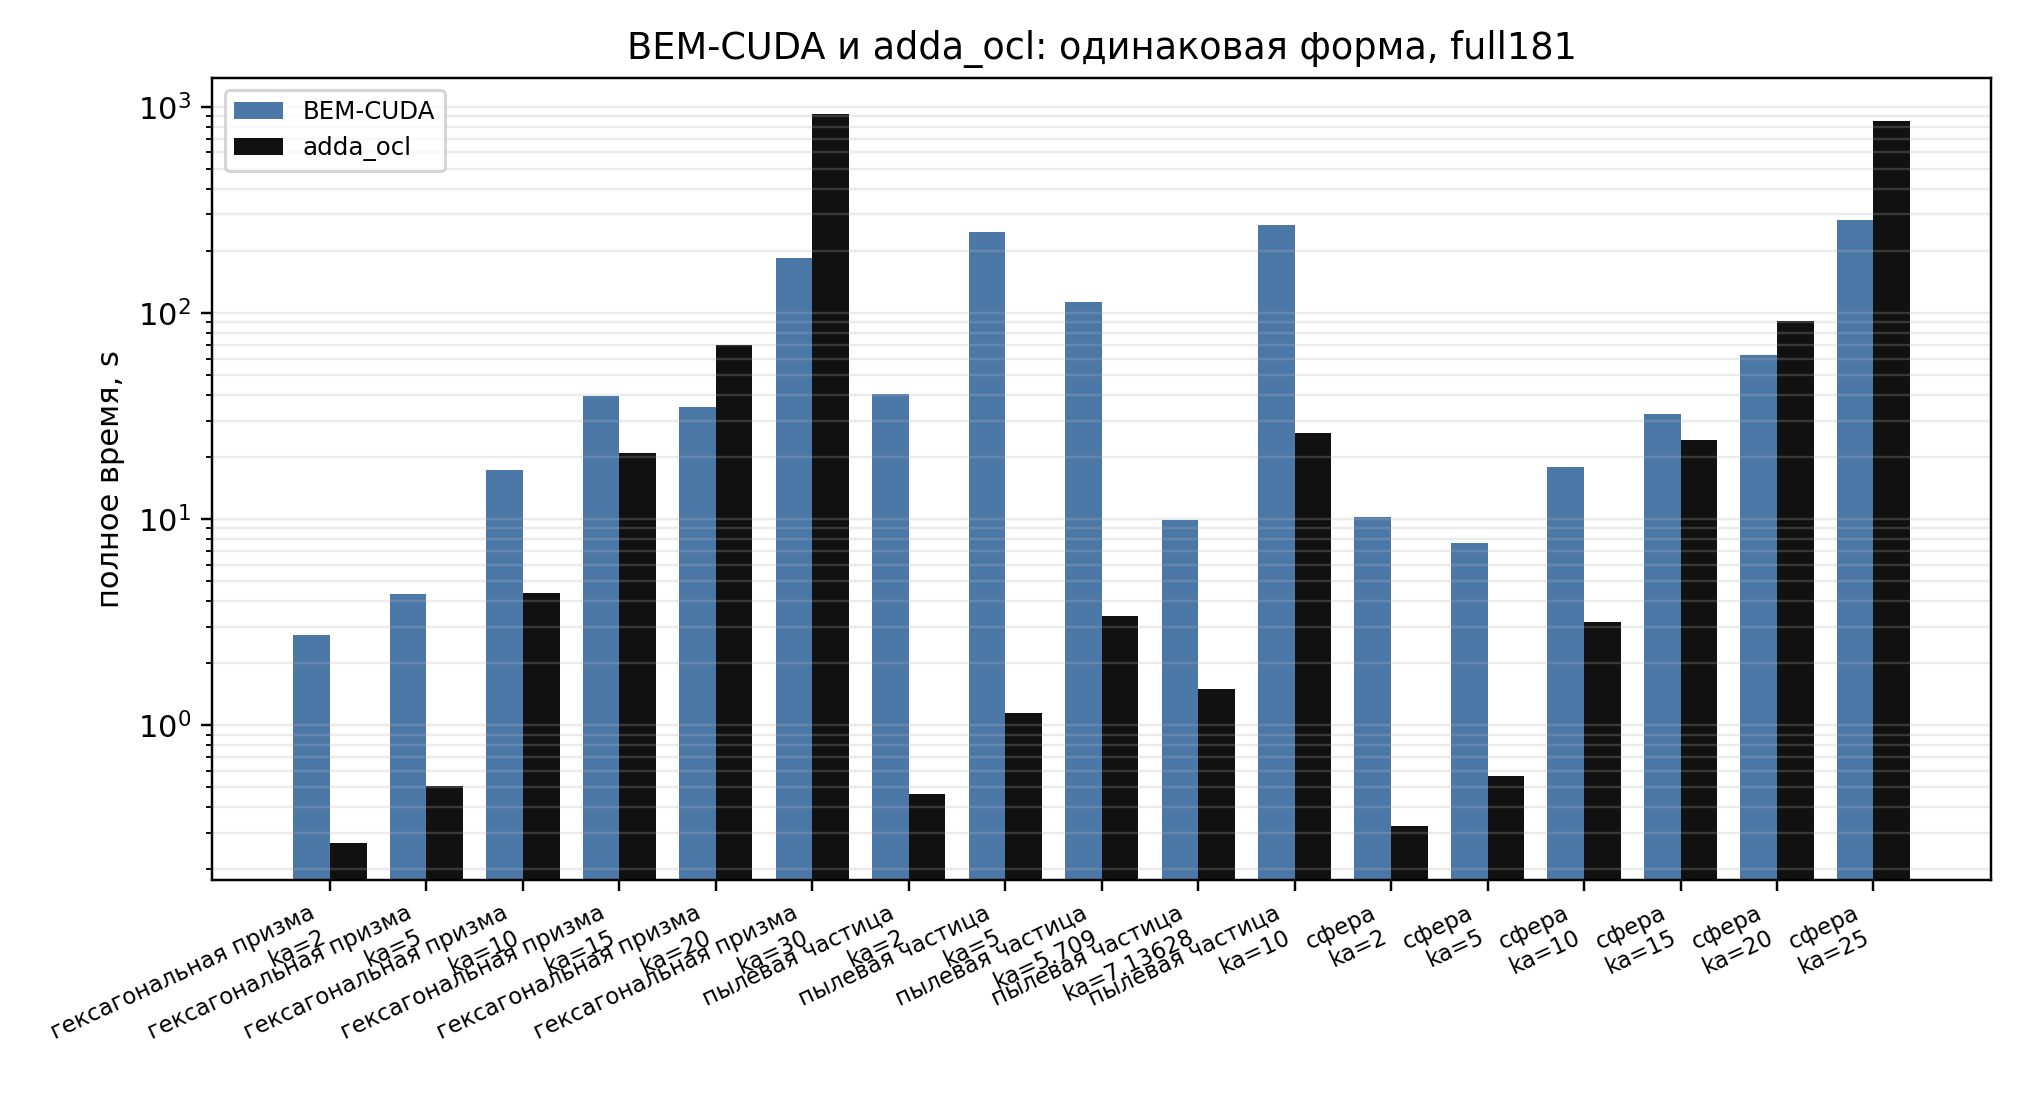
\includegraphics[width=0.96\textwidth,height=0.76\textheight,keepaspectratio]{fig_backend_comparison.png}
\caption{Сравнение вычислительных backend-ов при согласованной физической задаче.}
\end{figure}
Backend считается пригодным только после сравнения с плотным или более точным FMM на
той же сетке. Совпадение времени без совпадения матрицы Мюллера не имеет ценности.

\clearpage
\section{Память backend-ов}
\begin{figure}[H]\centering
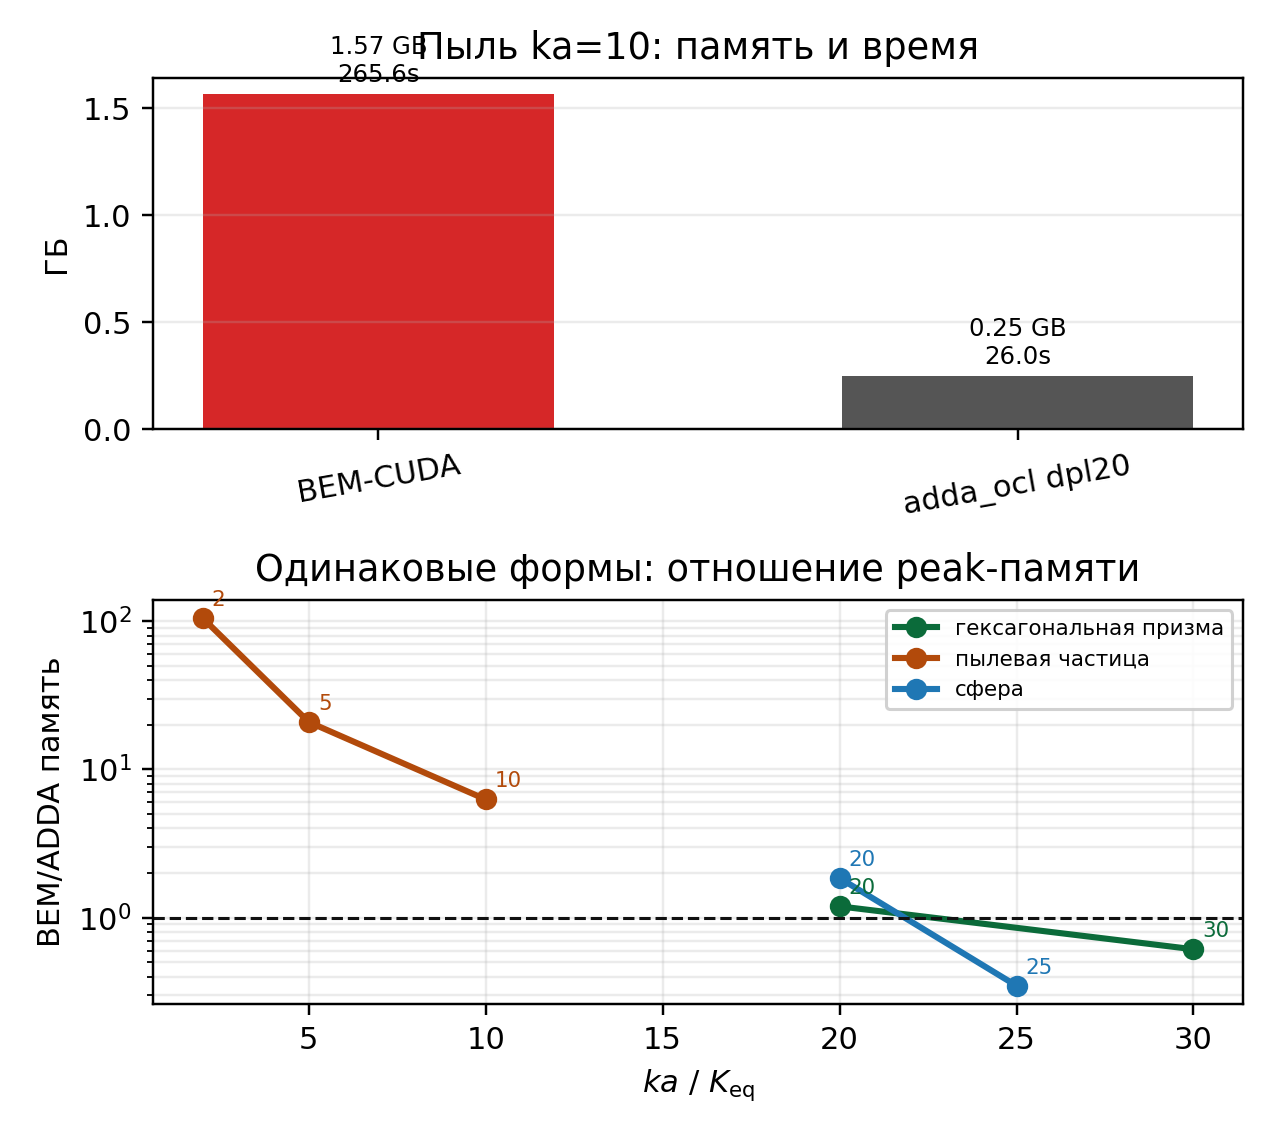
\includegraphics[width=0.96\textwidth,height=0.76\textheight,keepaspectratio]{fig_memory_backend_comparison.png}
\caption{Измеренная память разных backend-ов.}\end{figure}
Следует различать выделенную CUDA-память, пик процесса и суммарную память узла.
Прогноз за пределами измеренного диапазона маркируется как экстраполяция.

\clearpage
\section{Surface-pFFT}
\begin{figure}[H]\centering
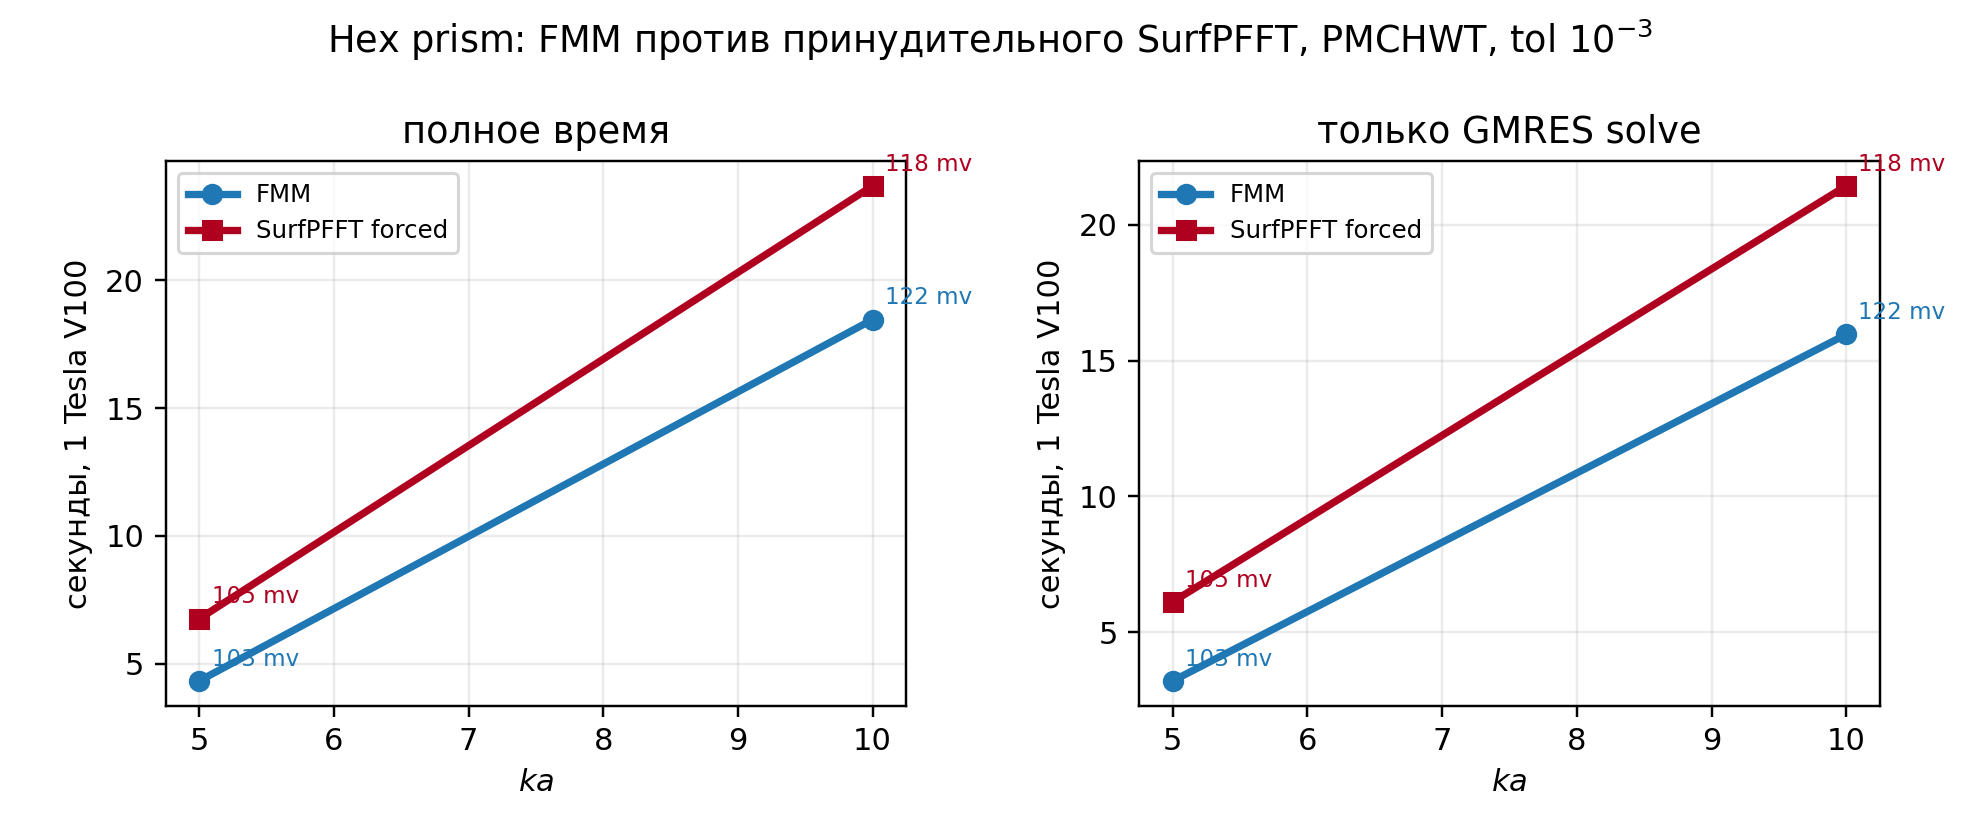
\includegraphics[width=0.96\textwidth,height=0.76\textheight,keepaspectratio]{fig_spfft_benchmark.png}
\caption{Экспериментальный Surface-pFFT относительно FMM.}\end{figure}
В текущем CLI \code{spfft} может откатываться на FMM. Метаданные результата должны
показывать фактически использованный backend, иначе график сравнивает названия команд,
а не алгоритмы.

\clearpage
\section{Ускоренное усреднение по $\alpha$}
\begin{figure}[H]\centering
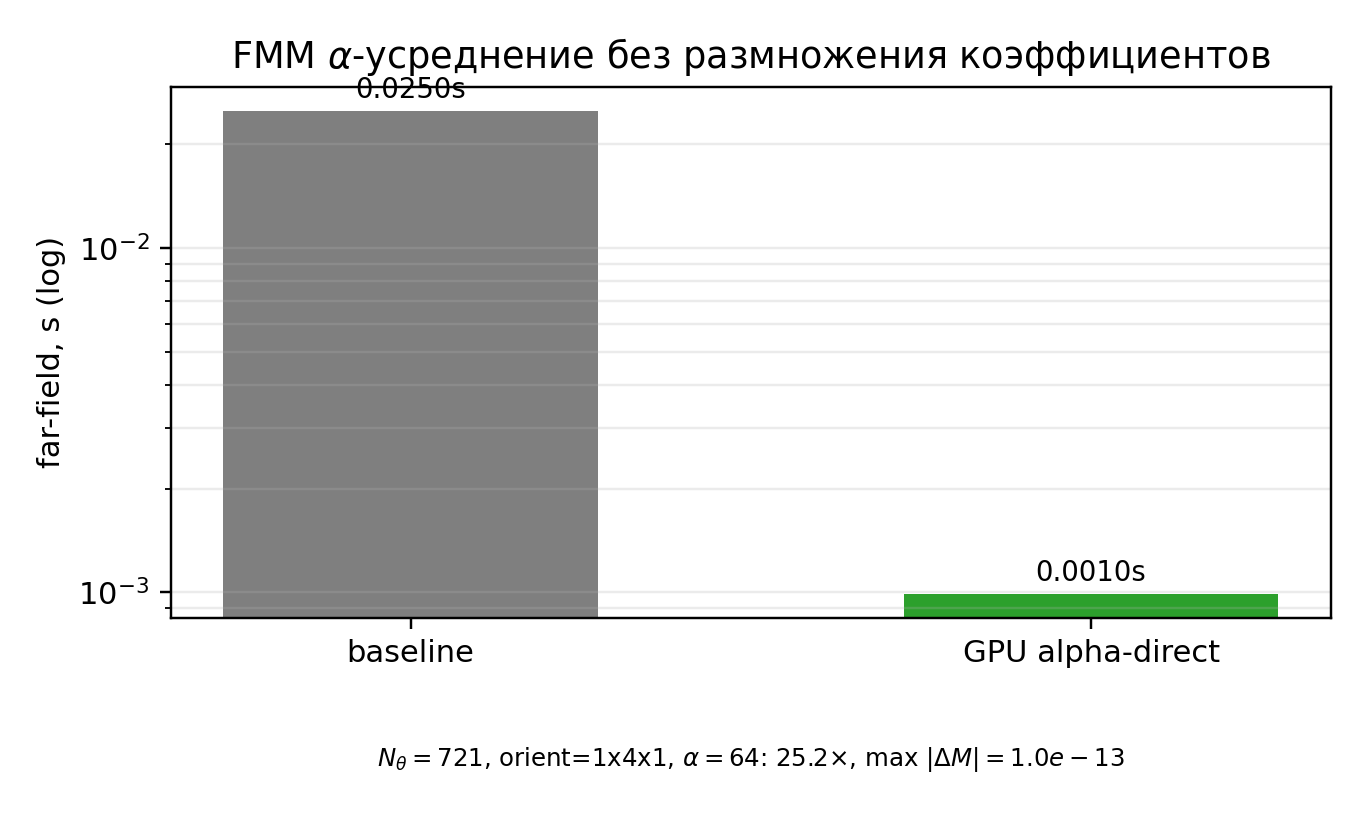
\includegraphics[width=0.96\textwidth,height=0.76\textheight,keepaspectratio]{fig_alpha_direct_benchmark.png}
\caption{Сравнение явного и ускоренного $\alpha$-усреднения.}\end{figure}
Правильность проверяется на одной и той же полной сетке углов Эйлера. Ускорение
оценивается после подтверждения равенства матрицы Мюллера, а не только $M_{11}$.

\clearpage
\section{Передача коэффициентов}
\begin{figure}[H]\centering
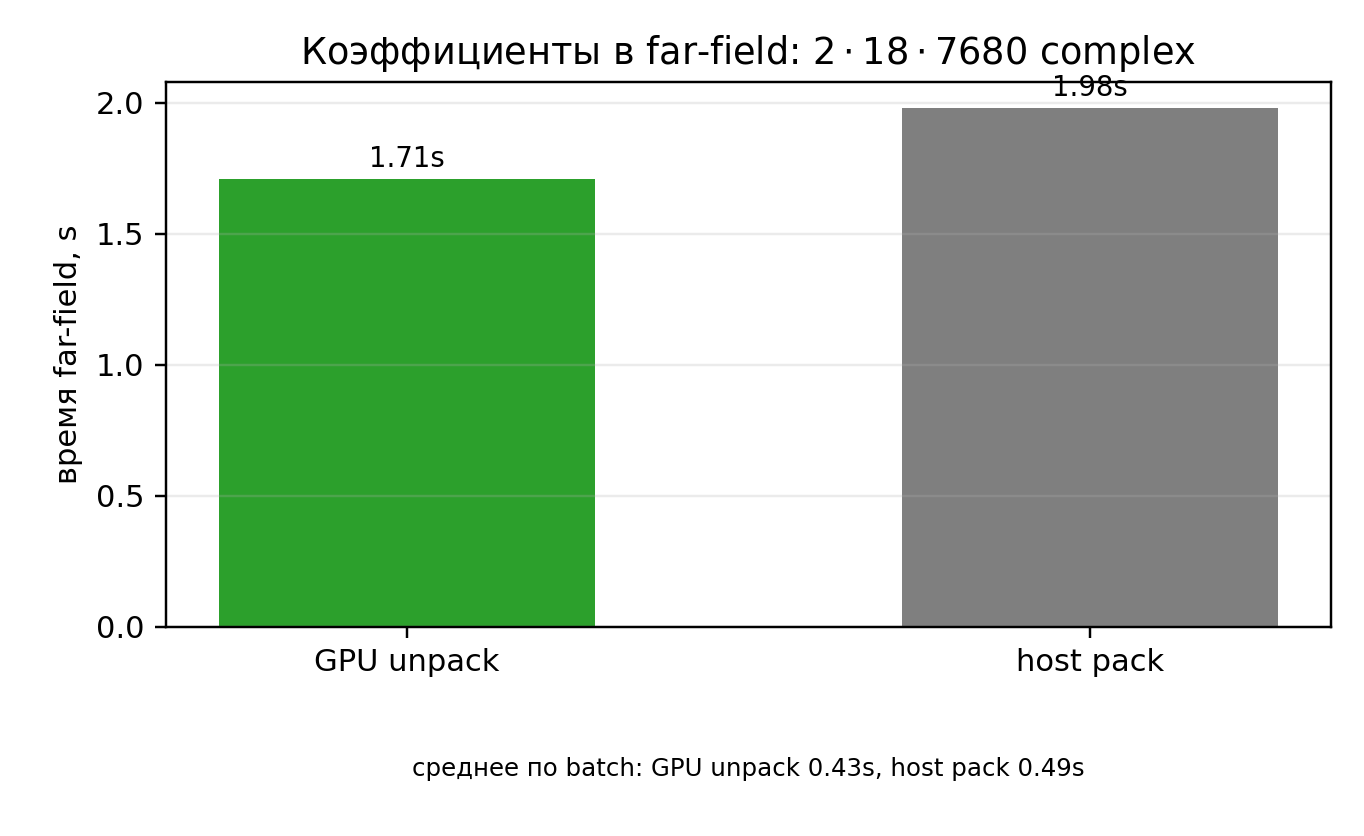
\includegraphics[width=0.96\textwidth,height=0.76\textheight,keepaspectratio]{fig_coeff_upload_benchmark.png}
\caption{Накладные расходы передачи коэффициентов токов на GPU.}\end{figure}
При большом числе ориентаций малая передача, повторяемая тысячи раз, становится
измеримой. Пакетирование уменьшает накладные расходы, но увеличивает рабочую память.

\clearpage
\section{Размер пылевой частицы}
\begin{figure}[H]\centering
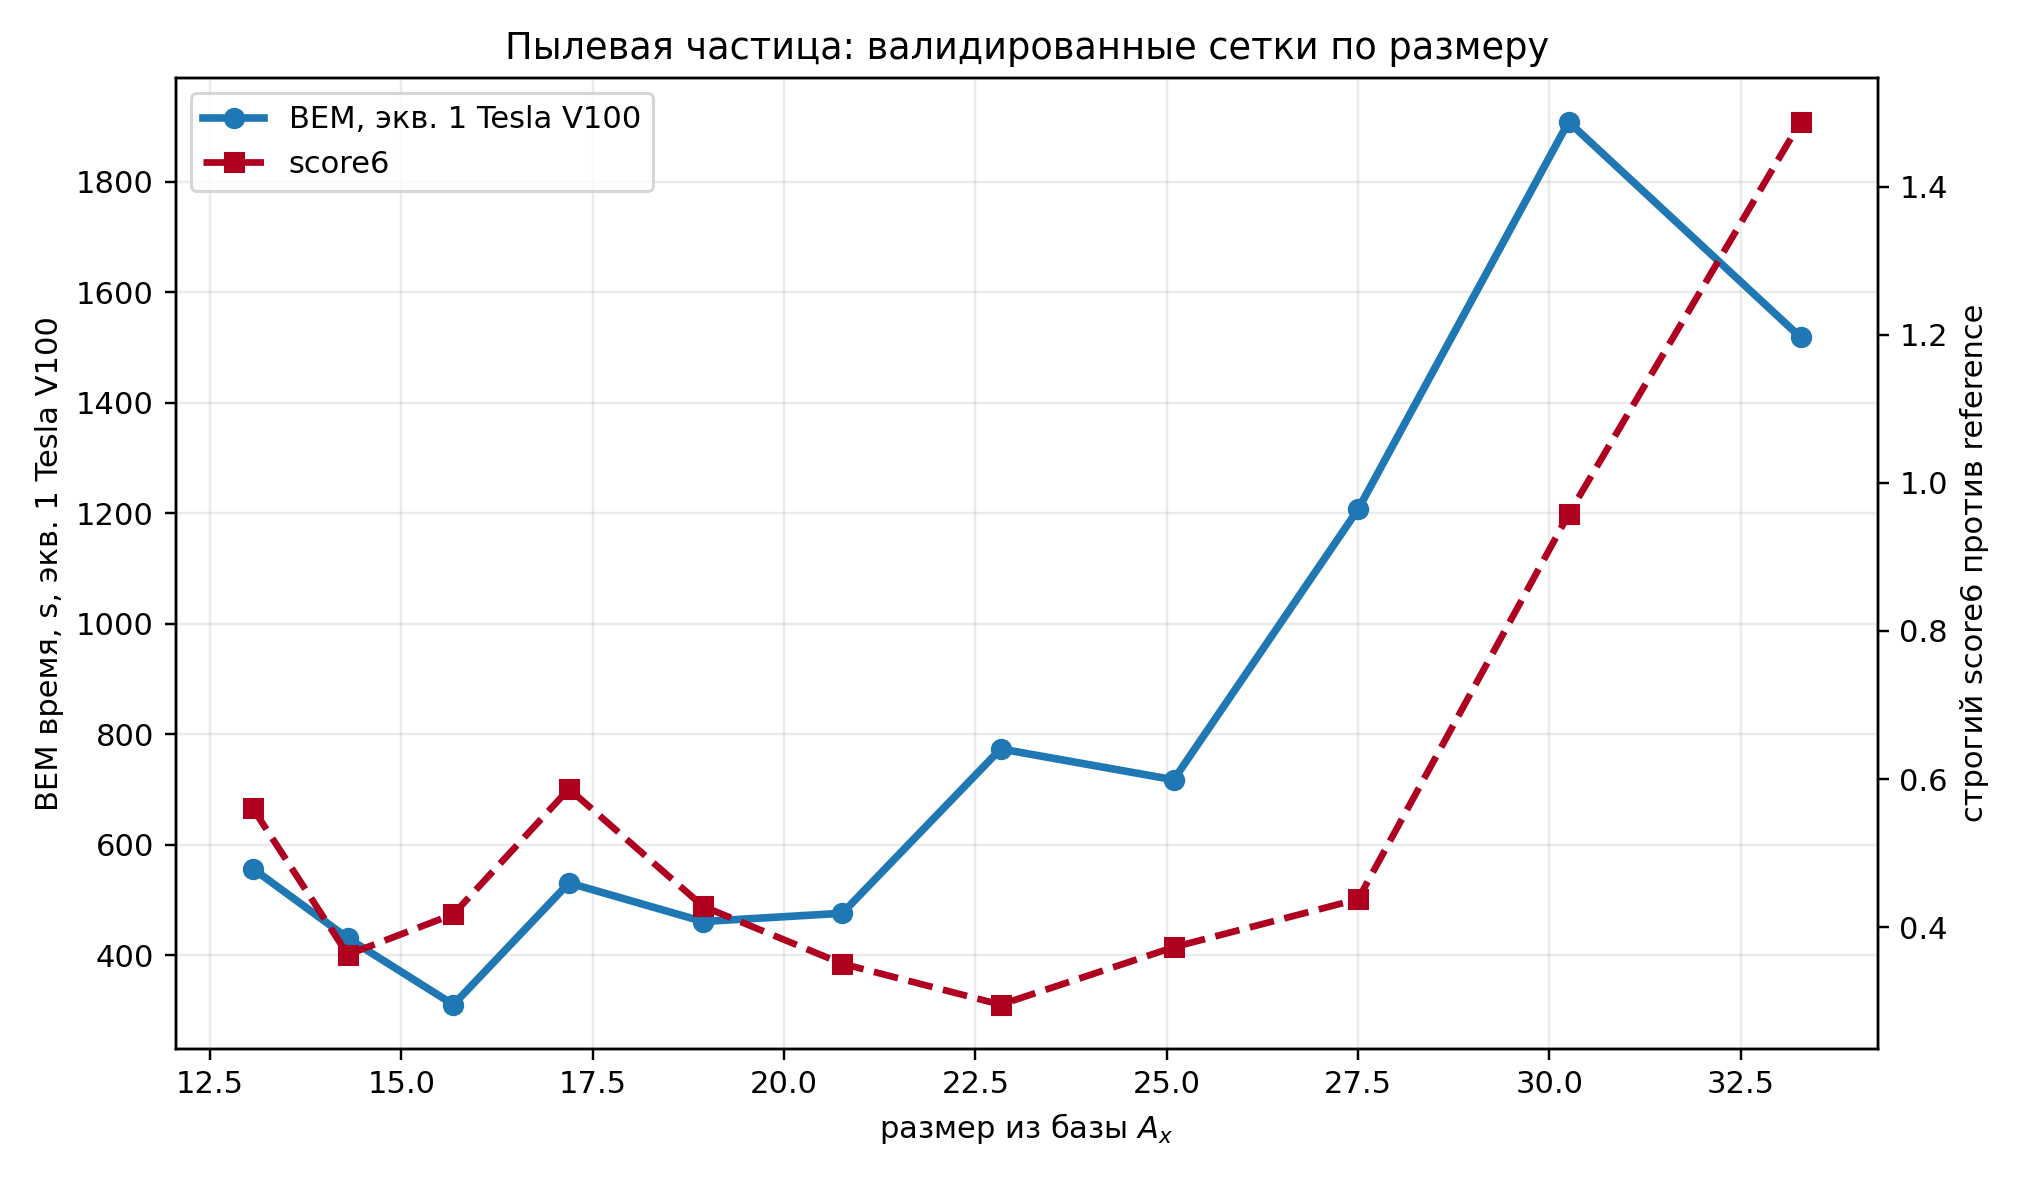
\includegraphics[width=0.96\textwidth,height=0.76\textheight,keepaspectratio]{fig_greek_size.png}
\caption{Серия размеров пылевой частицы.}\end{figure}
Для произвольной формы $ka$ не определяет единственное число треугольников. С ростом
размера одновременно меняются требования к поверхности, квадратуре и ориентациям.

\clearpage
\section{Совместная скорость и точность}
\begin{figure}[H]\centering
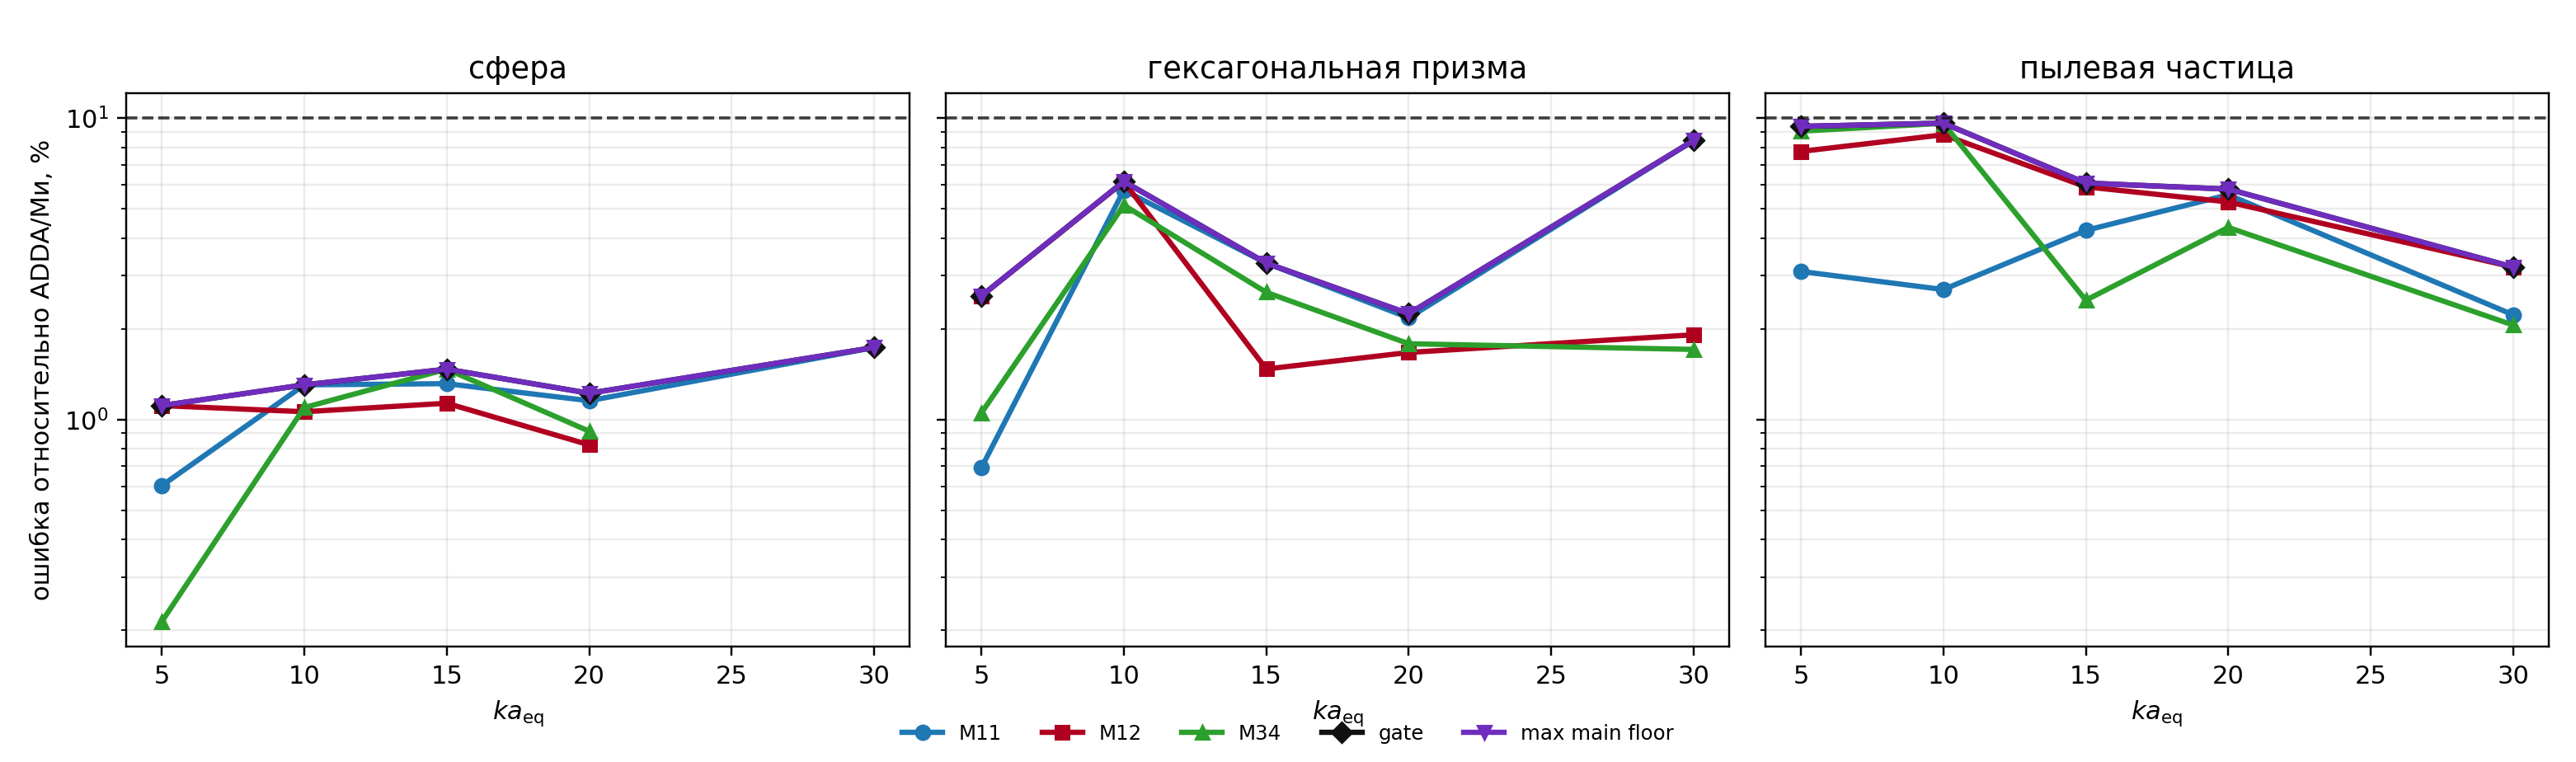
\includegraphics[width=0.96\textwidth,height=0.76\textheight,keepaspectratio]{fig_speed_pair_accuracy.png}
\caption{Совместное представление времени и ошибки.}\end{figure}
Оптимальной является точка на границе Парето. Выбор самого быстрого режима без
ограничения ошибки или самого точного без учёта ресурсов не решает практическую задачу.

\clearpage
\section{Большая сфера}
\begin{figure}[H]\centering
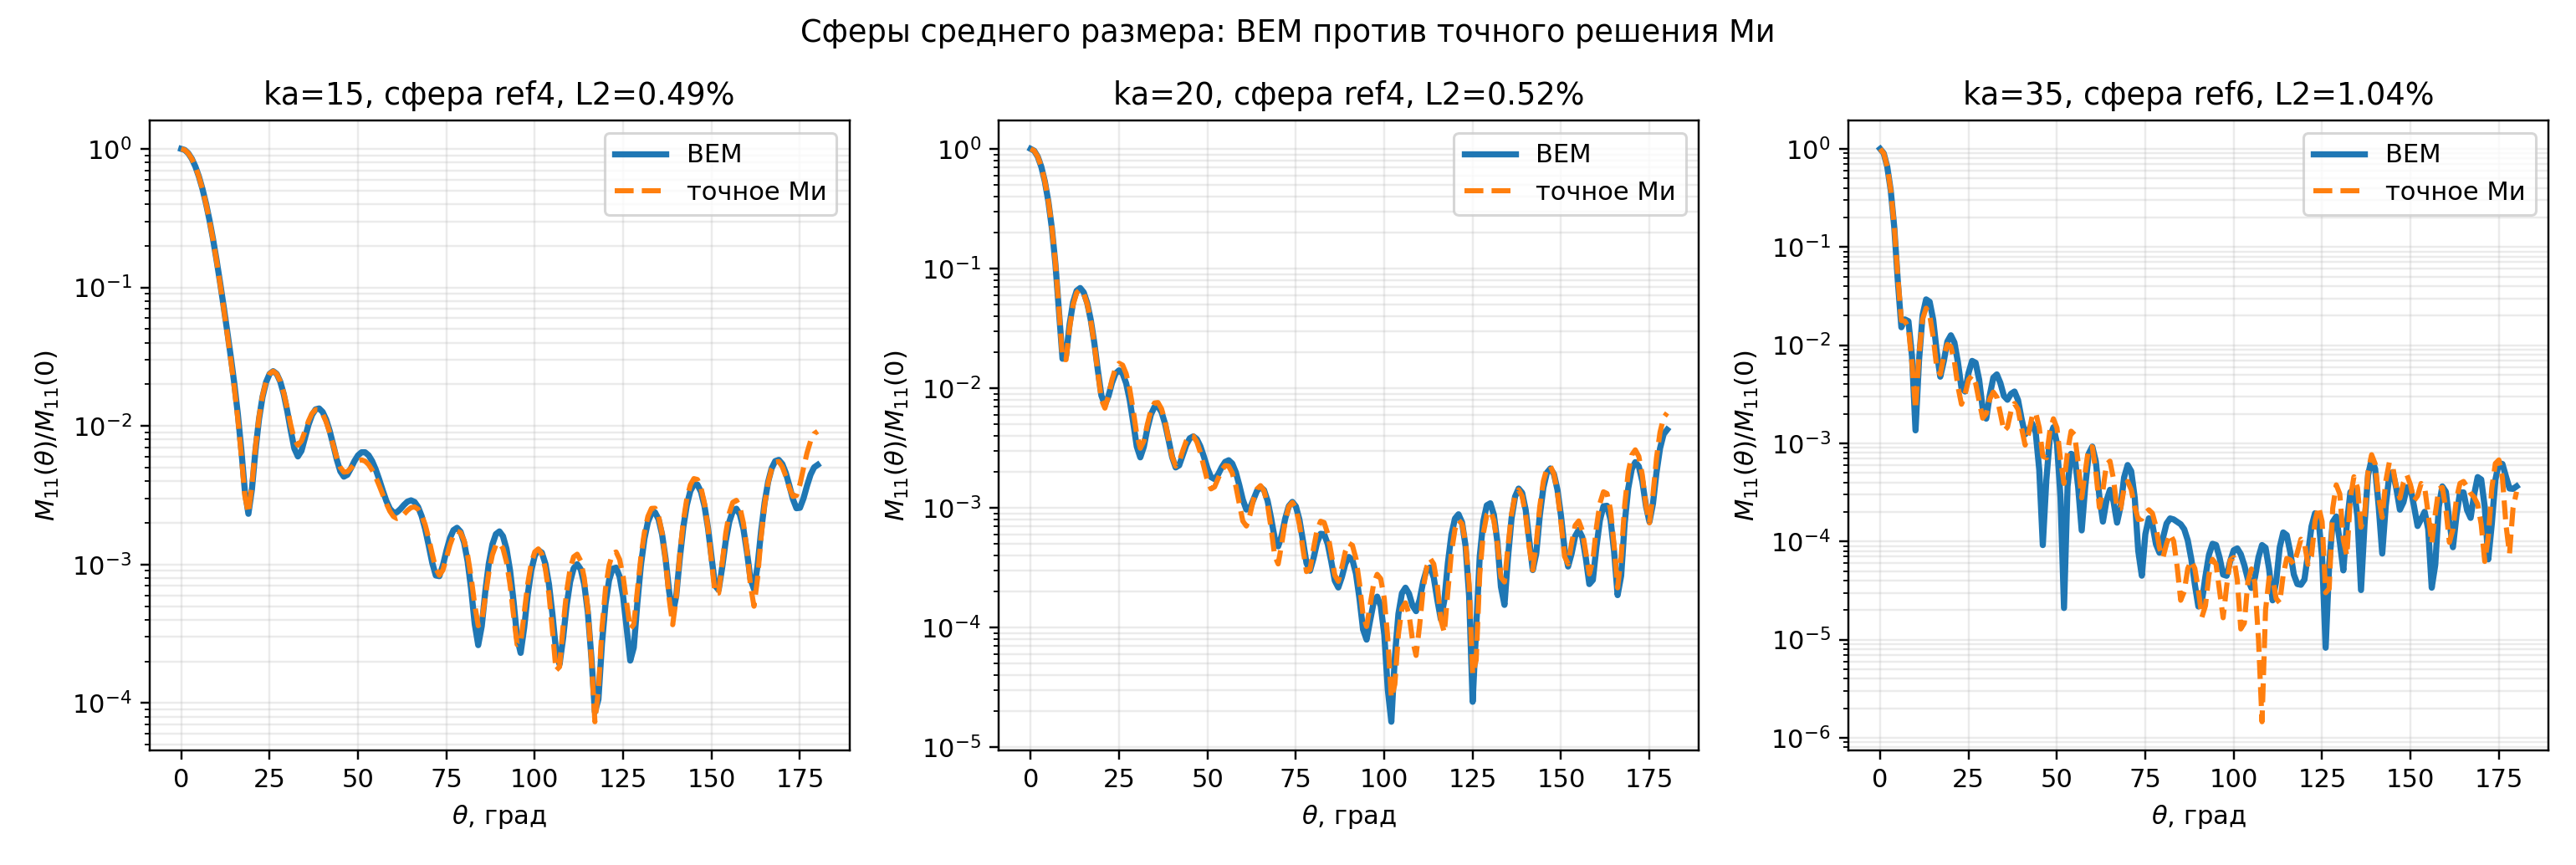
\includegraphics[width=0.96\textwidth,height=0.76\textheight,keepaspectratio]{fig_mie_large_reference.png}
\caption{Контроль большой сферы по теории Ми.}\end{figure}
Этот тест особенно чувствителен к угловому разрешению переднего пика и дисперсионной
ошибке поверхности. Ошибка $M_{11}$ оценивается с весом $\sin\theta$ и отдельно в
задней полусфере.

\clearpage
\section{Точность ADDA OpenCL}
\begin{figure}[H]\centering
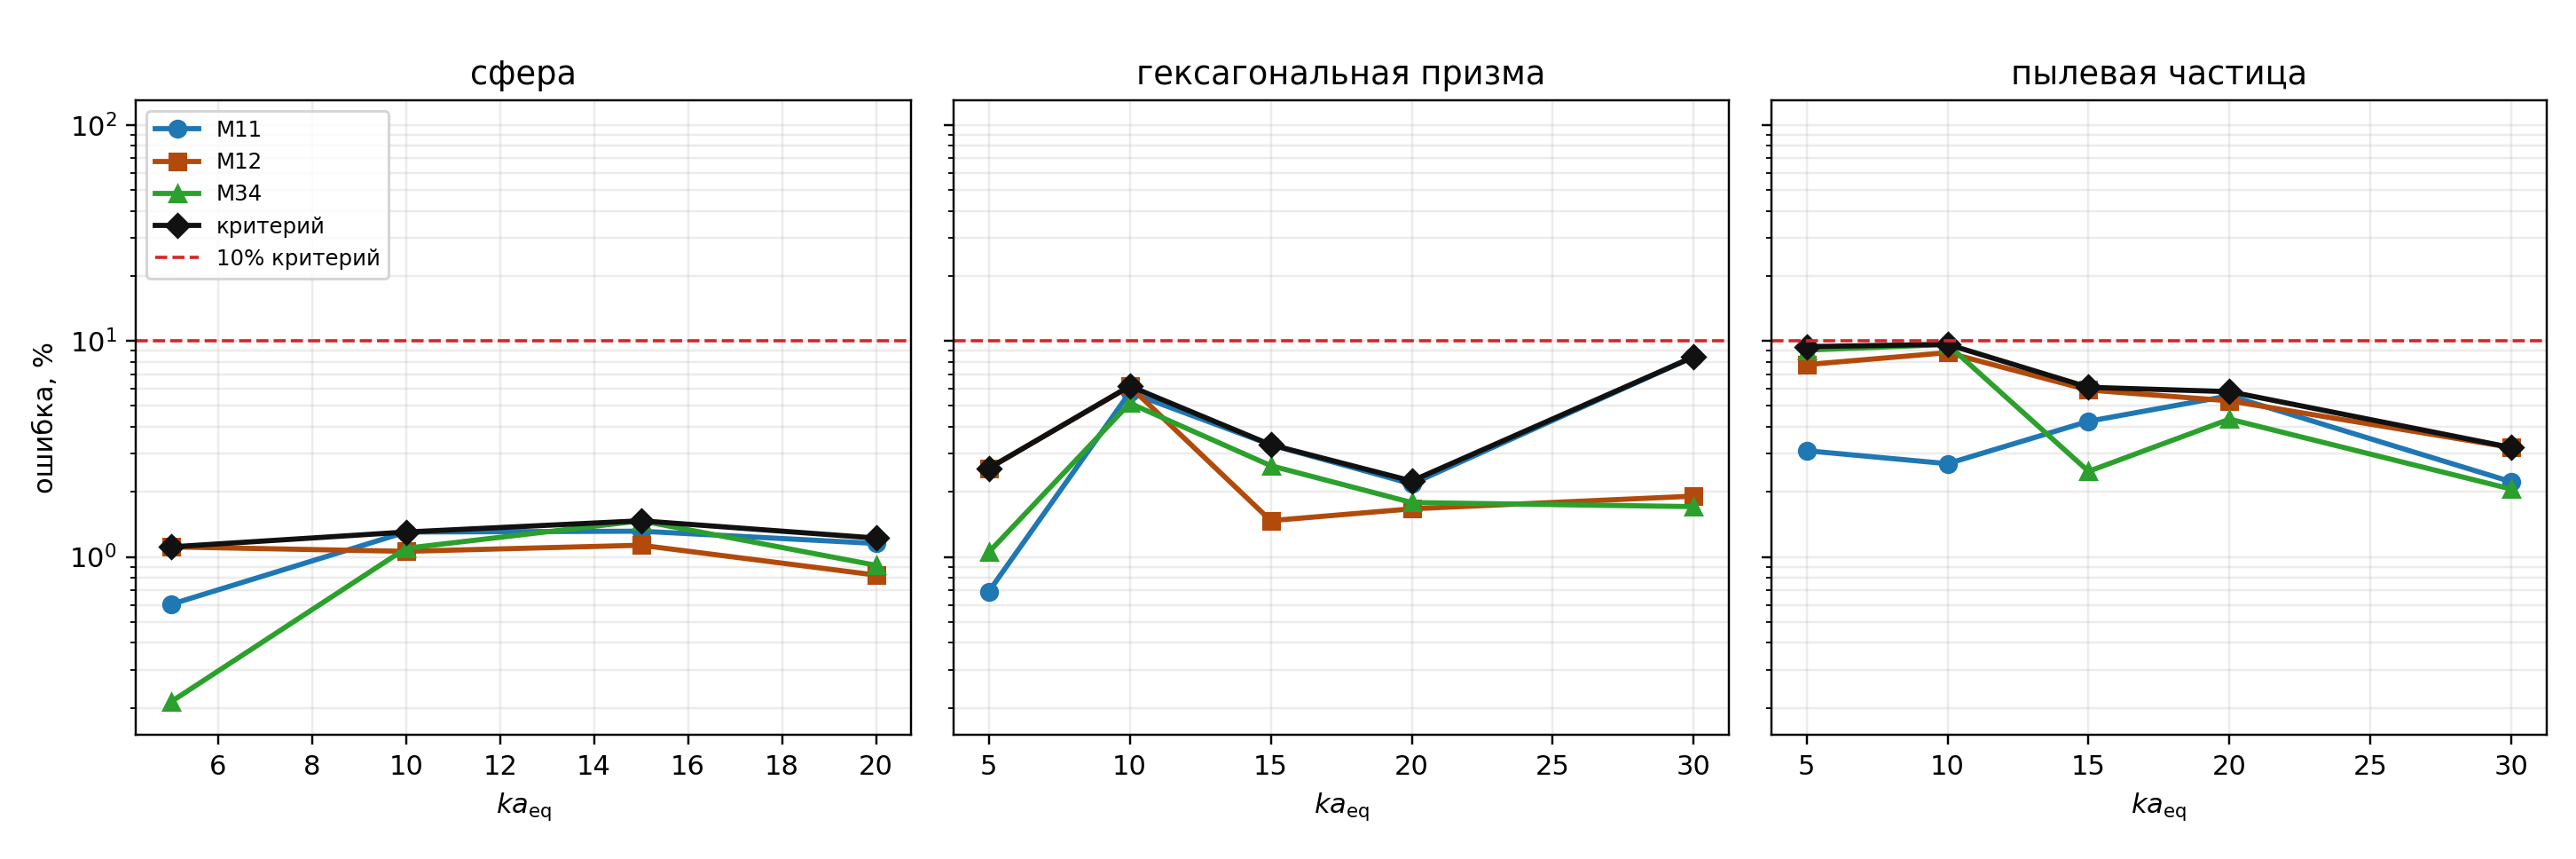
\includegraphics[width=0.96\textwidth,height=0.76\textheight,keepaspectratio]{fig_adda_ocl_accuracy.png}
\caption{Контроль эталонных расчётов \code{adda\_ocl}.}\end{figure}
ADDA не является точным решением для несферической частицы: его собственная сетка и
допуск также должны сходиться. Эталон выбирается из наиболее строгого завершённого
расчёта, а не из первого доступного файла.

\clearpage
\section{Профили сетки призмы}
\begin{figure}[H]\centering
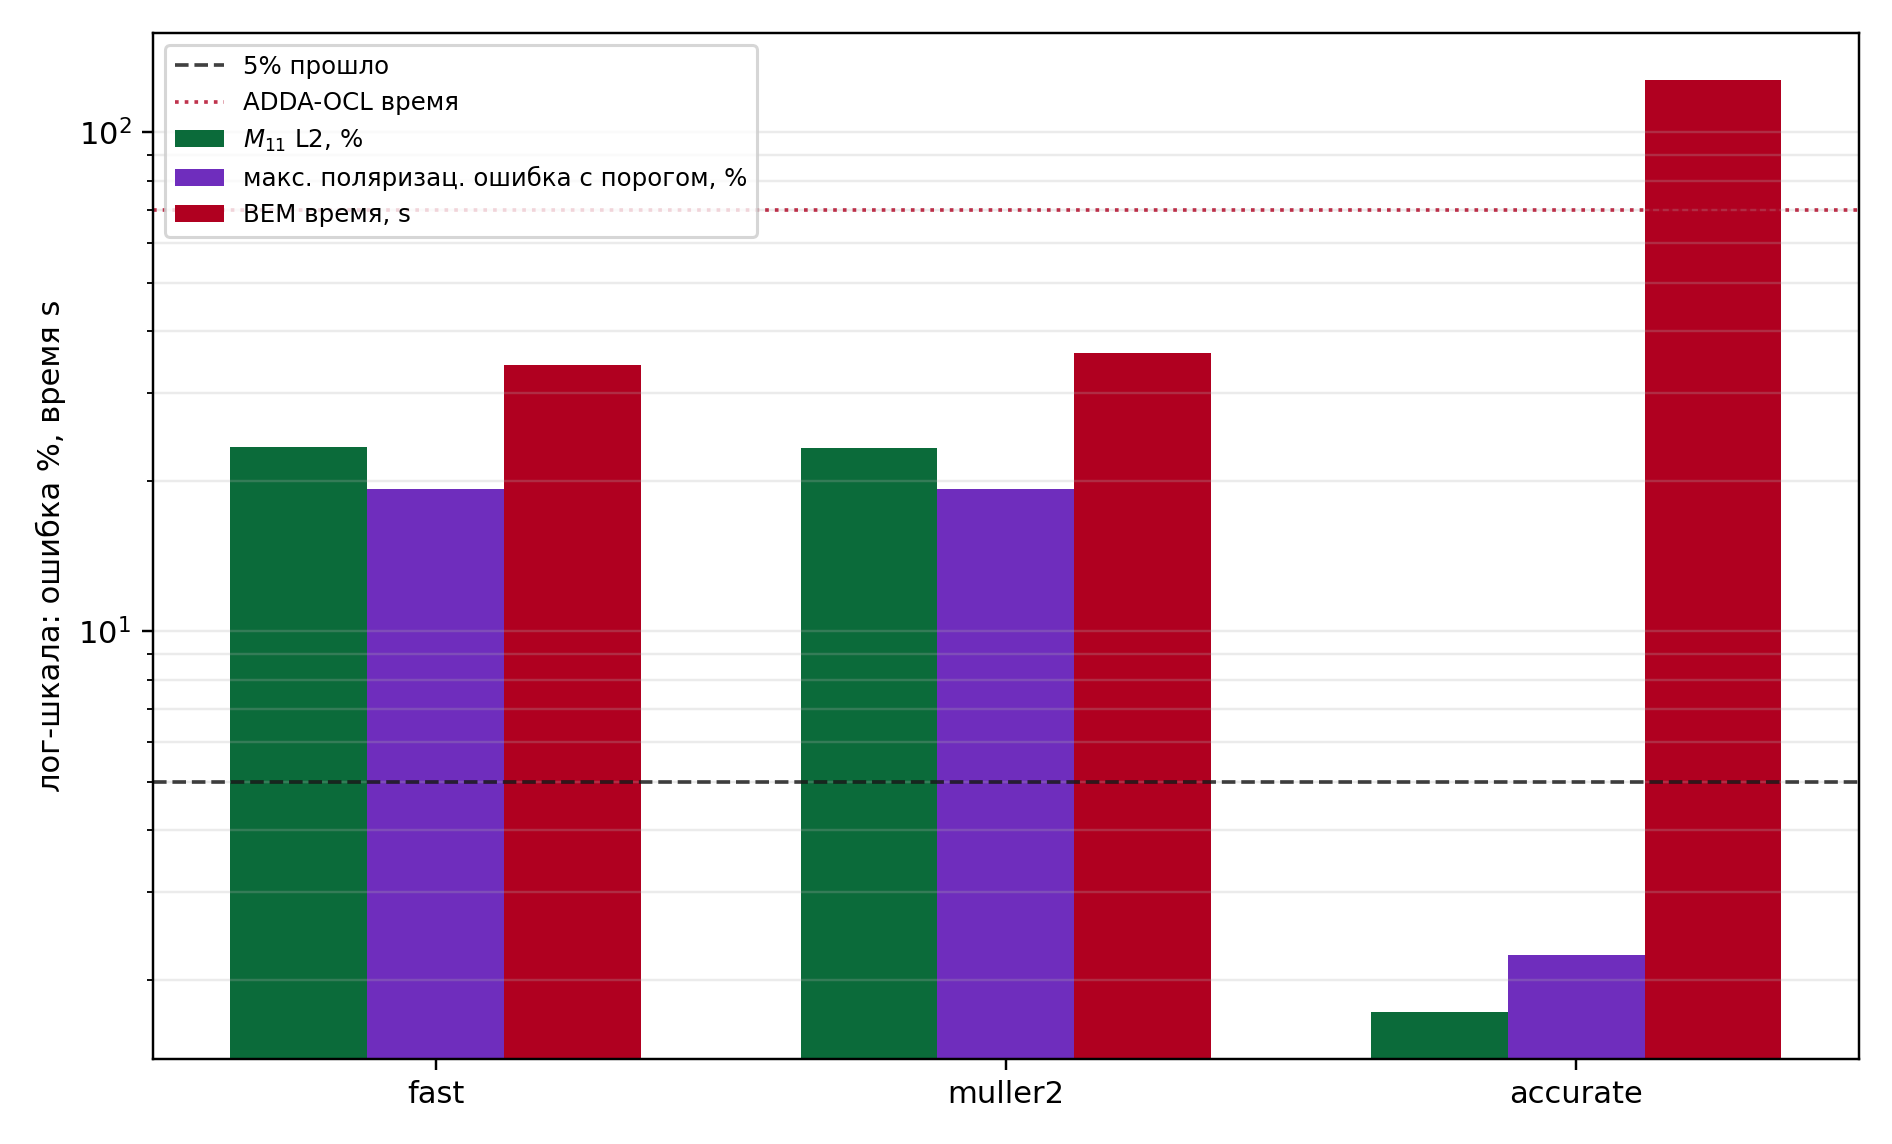
\includegraphics[width=0.96\textwidth,height=0.76\textheight,keepaspectratio]{fig_hex_accuracy_profile.png}
\caption{Профиль дискретизации призмы по диапазону размеров.}\end{figure}
Граница между уровнями ref определяется целевой ошибкой, а не круглым значением $ka$.
В переходной области проверяются оба уровня.

\clearpage
\section{Сканирование параметров пыли}
\begin{figure}[H]\centering
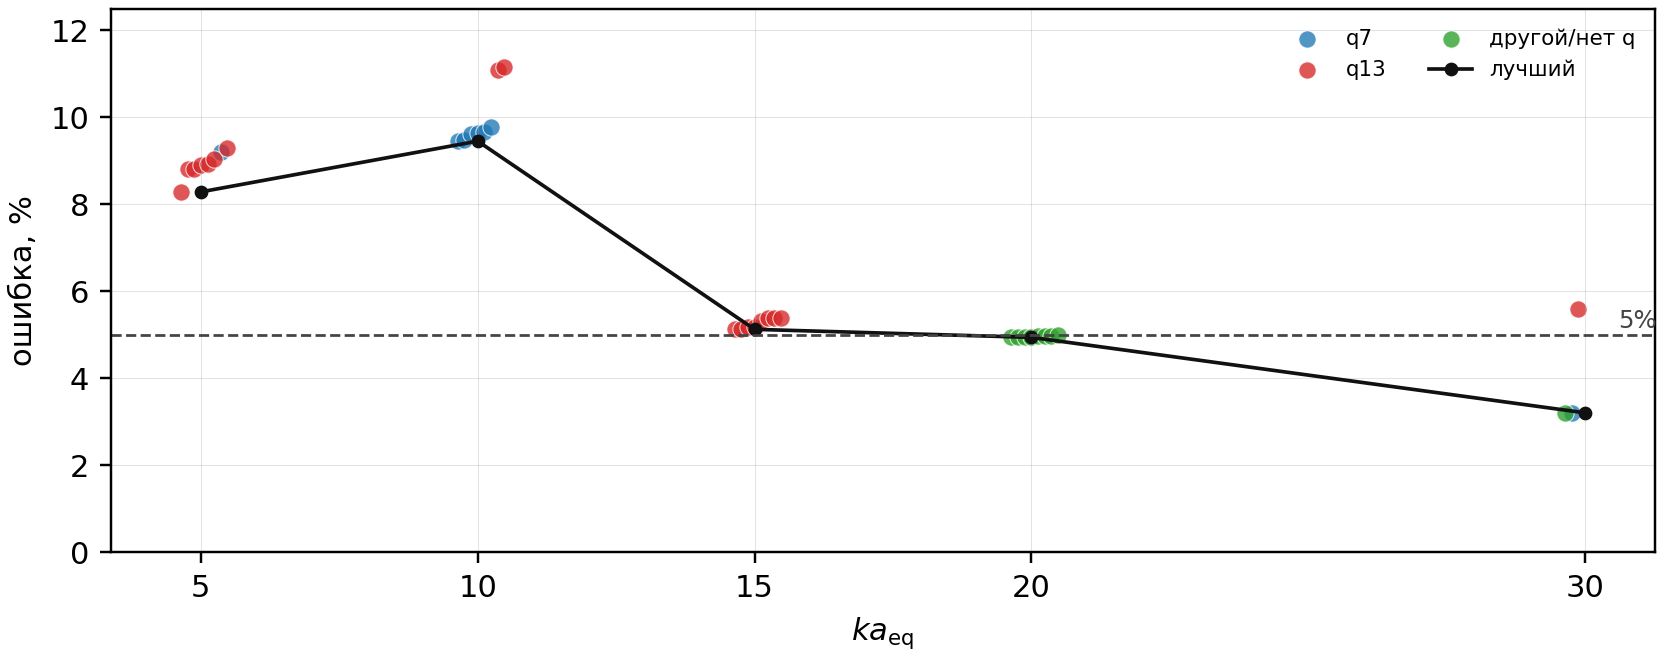
\includegraphics[width=0.96\textwidth,height=0.76\textheight,keepaspectratio]{fig_dust_candidate_parameter_scan.png}
\caption{Сканирование сетки, квадратуры и решателя для пылевой частицы.}\end{figure}
Сканирование используется для поиска кандидатов, но финальная точка пересчитывается
отдельно со строгими параметрами и полной ориентационной сеткой.

\clearpage
\section{Масштабирование по углам Эйлера}
\begin{figure}[H]\centering
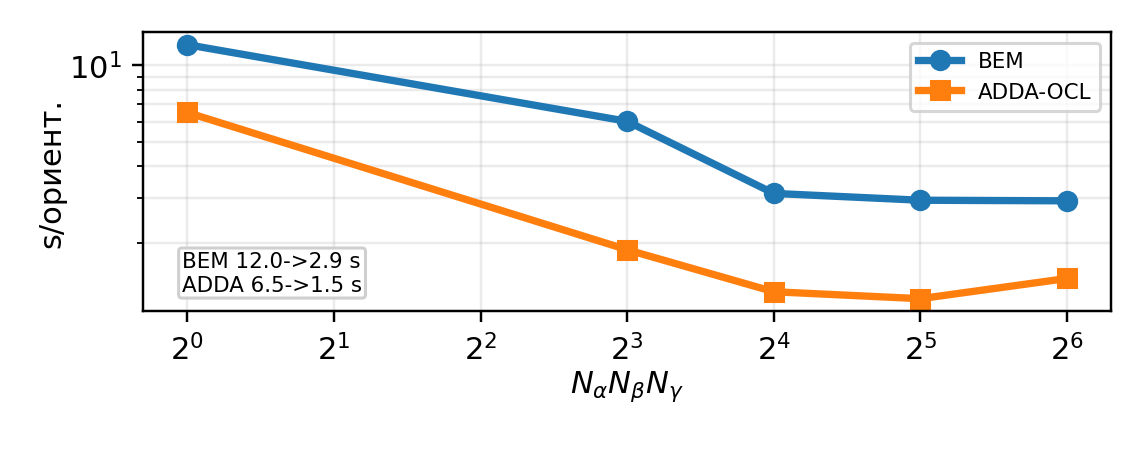
\includegraphics[width=0.96\textwidth,height=0.76\textheight,keepaspectratio]{fig_hex_euler_scaling.png}
\caption{Время и накладные расходы при росте числа ориентаций.}\end{figure}
При большом ансамбле доля инициализации FMM уменьшается, поскольку оператор используется
повторно. Для сравнения с ADDA учитываются одинаковое полное число ориентаций и число GPU.

\chapter{Машинно-читаемые таблицы экспериментов}
Ниже включены исходные CSV, на которых основаны ключевые рекомендации. Это позволяет
проверить числа без распознавания графиков. Столбцы могут содержать диагностические
точки; статус сходимости имеет приоритет над числовым значением времени.

\csvsection{Валидация по Ми}{manual_assets/table_mie_validation.csv}
\clearpage
\csvsection{Требуемый уровень сферической сетки}{manual_assets/table_sphere_ref_requirement.csv}
\clearpage
\csvsection{Память: эксперимент}{manual_assets/table_vram_experiment.csv}
\clearpage
\csvsection{Память: прогноз}{manual_assets/table_vram_forecast.csv}
\clearpage
\csvsection{Время одной ориентации}{manual_assets/table_shape_single_time.csv}
\clearpage
\csvsection{Пакетный FMM}{manual_assets/table_batch4_benchmark.csv}
\clearpage
\csvsection{Сравнение backend-ов}{manual_assets/table_backend_comparison.csv}
\clearpage
\csvsection{Сходимость пылевой частицы}{manual_assets/table_dust_fullgrid_compare.csv}
\clearpage
\csvsection{Сравнение BEM и ADDA OpenCL}{manual_assets/table_bem_vs_adda_ocl_same_shape.csv}
\clearpage
\csvsection{Ускоренное $\alpha$-усреднение}{manual_assets/table_alpha_direct_benchmark.csv}
\clearpage
\csvsection{Требования к сетке по размеру}{manual_assets/table_mesh_level_requirement.csv}
\clearpage
\csvsection{Совместная скорость и точность}{manual_assets/table_speed_pair_accuracy_by_shape.csv}
\clearpage
\csvsection{Память backend-ов на одной форме}{manual_assets/table_memory_backend_same_shape.csv}
\clearpage
\csvsection{Предобуславливатель призмы}{manual_assets/table_hex_precond_benchmark.csv}
\clearpage
\csvsection{Sweep по показателю преломления}{manual_assets/table_index_sweep.csv}
\clearpage
\csvsection{Точность ADDA OpenCL}{manual_assets/table_adda_ocl_accuracy.csv}
\clearpage

\chapter{Литература и дальнейшее чтение}
\begin{thebibliography}{99}
\bibitem{PMCHWT1} A.~J.~Poggio, E.~K.~Miller. Integral equation solutions of
three-dimensional scattering problems. In: \emph{Computer Techniques for
Electromagnetics}, 1973.
\bibitem{PMCHWT2} Y.~Chang, R.~F.~Harrington. A surface formulation for characteristic
modes of material bodies. \emph{IEEE Trans. Antennas Propag.}, 25, 1977.
\bibitem{PMCHWT3} T.~K.~Wu, L.~L.~Tsai. Scattering from arbitrarily-shaped lossy
dielectric bodies of revolution. \emph{Radio Science}, 12, 1977.
\bibitem{RWG} S.~M.~Rao, D.~R.~Wilton, A.~W.~Glisson. Electromagnetic scattering by
surfaces of arbitrary shape. \emph{IEEE Trans. Antennas Propag.}, 30(3), 1982.
\bibitem{Chew} W.~C.~Chew. \emph{Waves and Fields in Inhomogeneous Media}. IEEE Press.
\bibitem{Nedelec} J.-C.~Nedelec. \emph{Acoustic and Electromagnetic Equations}.
Springer, 2001.
\bibitem{FMM} V.~Rokhlin. Rapid solution of integral equations of scattering theory in
two dimensions. \emph{J. Comput. Phys.}, 86, 1990.
\bibitem{MLFMA} J.~Song, C.-C.~Lu, W.~C.~Chew. Multilevel fast multipole algorithm for
electromagnetic scattering. \emph{IEEE Trans. Antennas Propag.}, 45, 1997.
\bibitem{GMRES} Y.~Saad, M.~H.~Schultz. GMRES: a generalized minimal residual algorithm.
\emph{SIAM J. Sci. Stat. Comput.}, 7, 1986.
\bibitem{QMR} R.~W.~Freund, N.~M.~Nachtigal. An implementation of QMR based on coupled
two-term recurrences. \emph{SIAM J. Sci. Comput.}, 15, 1994.
\bibitem{ADDAmanual} M.~A.~Yurkin, A.~G.~Hoekstra. User manual for the discrete dipole
approximation code ADDA 1.4.0, 2020.
\bibitem{DDAreview} M.~A.~Yurkin, A.~G.~Hoekstra. The discrete-dipole-approximation code
ADDA: capabilities and known limitations. \emph{JQSRT}, 112, 2011.
\end{thebibliography}

\backmatter
\chapter*{Заключение}
BEM-CUDA предоставляет специализированный GPU-путь для поверхностного решения задачи
рассеяния. Его сильная сторона --- отсутствие объёмной сетки и возможность повторно
использовать оператор для множества ориентаций. Основные ограничения --- качество
треугольной поверхности, плотность не локального оператора и сложность итерационной
сходимости. Надёжный результат получается не одной ``лучшей'' комбинацией флагов, а
последовательным контролем каждого слоя ошибки.

\end{document}
